\documentclass[report.tex]{subfiles}
\graphicspath{ \subfix{./images/} \subfix{./graphs/} }
\begin{document}
\section{Milestone 1: Create the UI}

\subsection{Objective}

During this milestone, a basic prototype with user interface will be created. The prototype needs to compile and run and the user should be able to navigate around the app to see different UI elements.

\subsection{Create a minimal running prototype}

\subsubsection{Implementation}

I will create a prototype with a minimal user interface to test run the development environment and building tools.\cite{microsoft:docs:create-your-first-winui3-app}

I create the \code{App.xaml} file, which will include all application resources. Right now, the only resources imported is the \code{XamlControlsResource}, which provides the resources for the all controls. Later on, I will create and import new resources in this file.

\begin{minted}{xml}
<Application
    x:Class="Algorithm_Dynamics.App"
    xmlns="http://schemas.microsoft.com/winfx/2006/xaml/presentation"
    xmlns:x="http://schemas.microsoft.com/winfx/2006/xaml"
    xmlns:local="using:Algorithm_Dynamics">
    <Application.Resources>
        <ResourceDictionary>
            <ResourceDictionary.MergedDictionaries>
                <XamlControlsResources xmlns="using:Microsoft.UI.Xaml.Controls" />
                <!-- Other merged dictionaries here -->
            </ResourceDictionary.MergedDictionaries>
            <!-- Other app resources here -->
        </ResourceDictionary>
    </Application.Resources>
</Application>
\end{minted}

I then create the \code{App.xaml.cs} file, which will include the main entry point of the application. It inheriates from the \code{Application} class, and create a \code{Window} object to show the main window. The \code{App} class will activate the main window when it is launched.

\begin{minted}{csharp}
using Microsoft.UI.Xaml;

namespace Algorithm_Dynamics
{
    /// <summary>
    /// Provides application-specific behavior to supplement the default Application class.
    /// </summary>
    public partial class App : Application
    {
        /// <summary>
        /// Initializes the singleton application object.  This is the first line of authored code
        /// executed, and as such is the logical equivalent of main() or WinMain().
        /// </summary>
        public App()
        {
            InitializeComponent();
        }

        /// <summary>
        /// Invoked when the application is launched normally by the end user.  Other entry points
        /// will be used such as when the application is launched to open a specific file.
        /// </summary>
        /// <param name="args">Details about the launch request and process.</param>
        protected override void OnLaunched(LaunchActivatedEventArgs args)
        {
            m_window = new MainWindow();
            m_window.Activate();
        }

        private Window m_window;
    }
}
\end{minted}

Next, I create the \code{MainWindow.xaml} file, which includes the layout of the main window. Right now, it only has a stack panel and a button inside to test everything is working.

\begin{minted}{xml}
<Window
    x:Class="Algorithm_Dynamics.MainWindow"
    xmlns="http://schemas.microsoft.com/winfx/2006/xaml/presentation"
    xmlns:x="http://schemas.microsoft.com/winfx/2006/xaml"
    xmlns:local="using:Algorithm_Dynamics"
    xmlns:d="http://schemas.microsoft.com/expression/blend/2008"
    xmlns:mc="http://schemas.openxmlformats.org/markup-compatibility/2006"
    mc:Ignorable="d">

    <StackPanel 
        Orientation="Horizontal" 
        HorizontalAlignment="Center" 
        VerticalAlignment="Center">
        <Button 
            x:Name="myButton"
            Click="myButton_Click"
            Content="Click Me"/>
    </StackPanel>
</Window>
\end{minted}

Finally, I create the \code{MainWindow.xaml.cs} file. It contains all the UI logic. In this prototype, when the button in the UI is clicked, its text will be changed to ``Clicked''.

\begin{minted}{csharp}
using Microsoft.UI.Xaml;

namespace Algorithm_Dynamics
{
    /// <summary>
    /// The main window object that is used to display all other elements
    /// </summary>
    public sealed partial class MainWindow : Window
    {
        public MainWindow()
        {
            InitializeComponent();
        }

        private void myButton_Click(object sender, RoutedEventArgs e)
        {
            myButton.Content = "Clicked";
        }
    }
}
\end{minted}

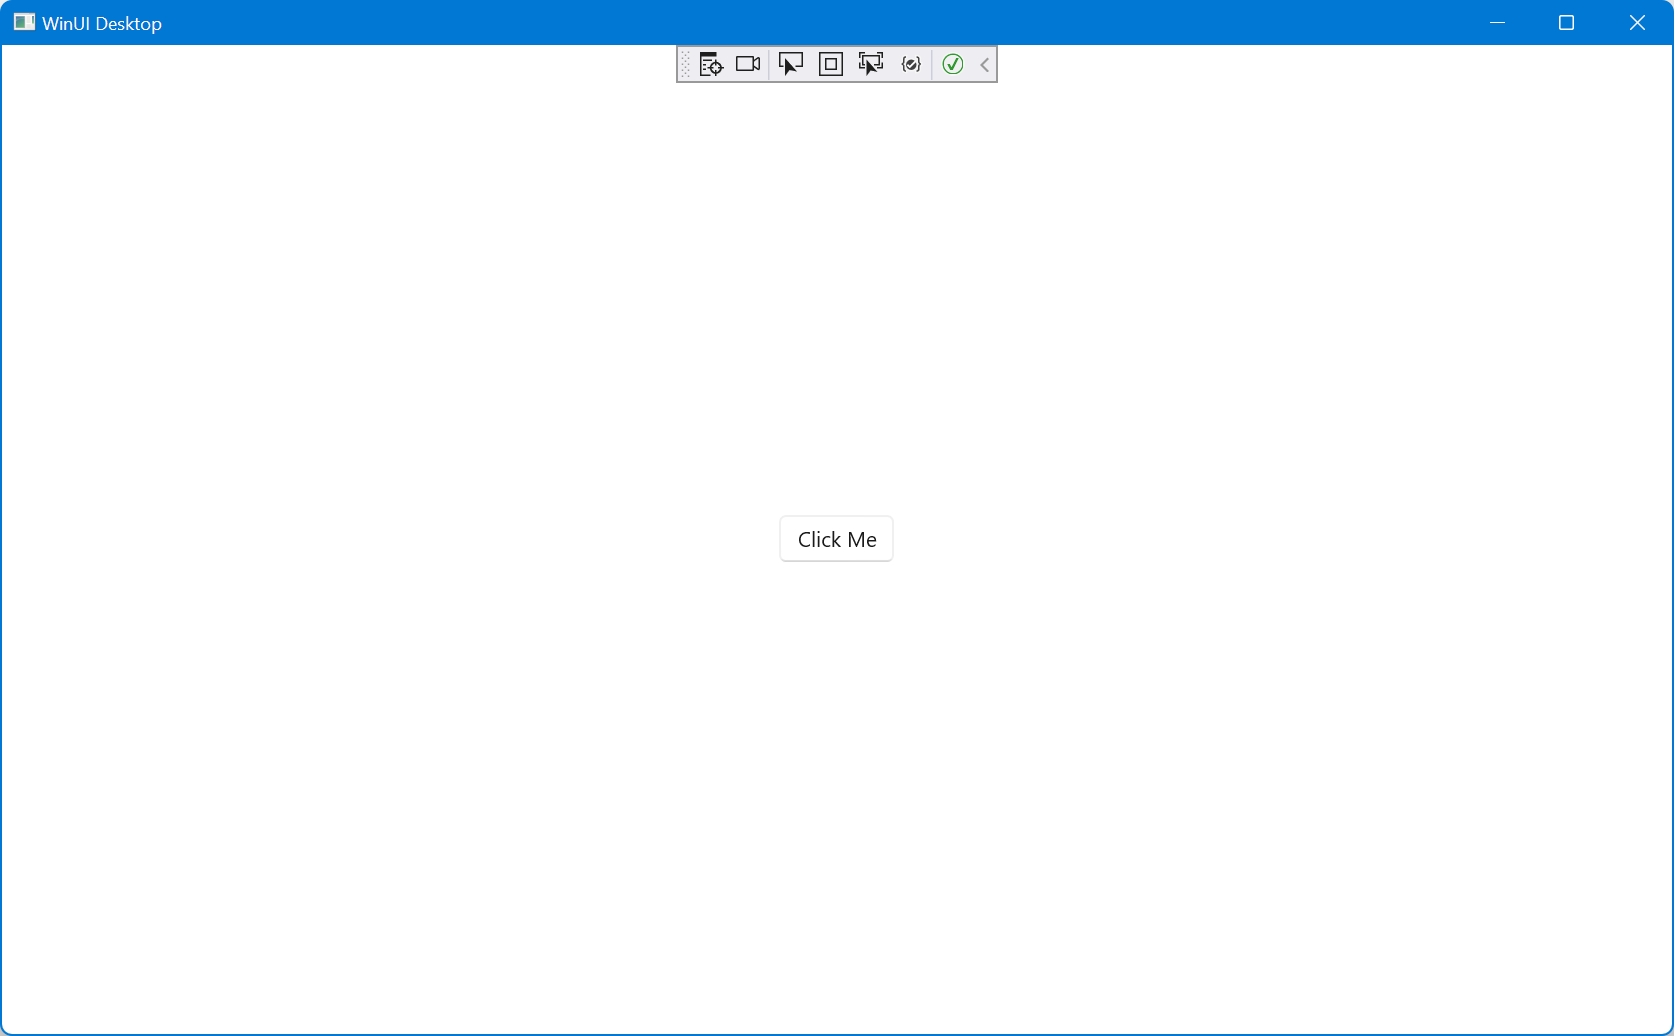
\includegraphics[width=\textwidth, height=\textheight, keepaspectratio]{Prototype-Button-Click-Me.png}

As expected, a window with a button shows up correctly. After clicking the button, the content in the button is changed to ``Clicked'' correctly.

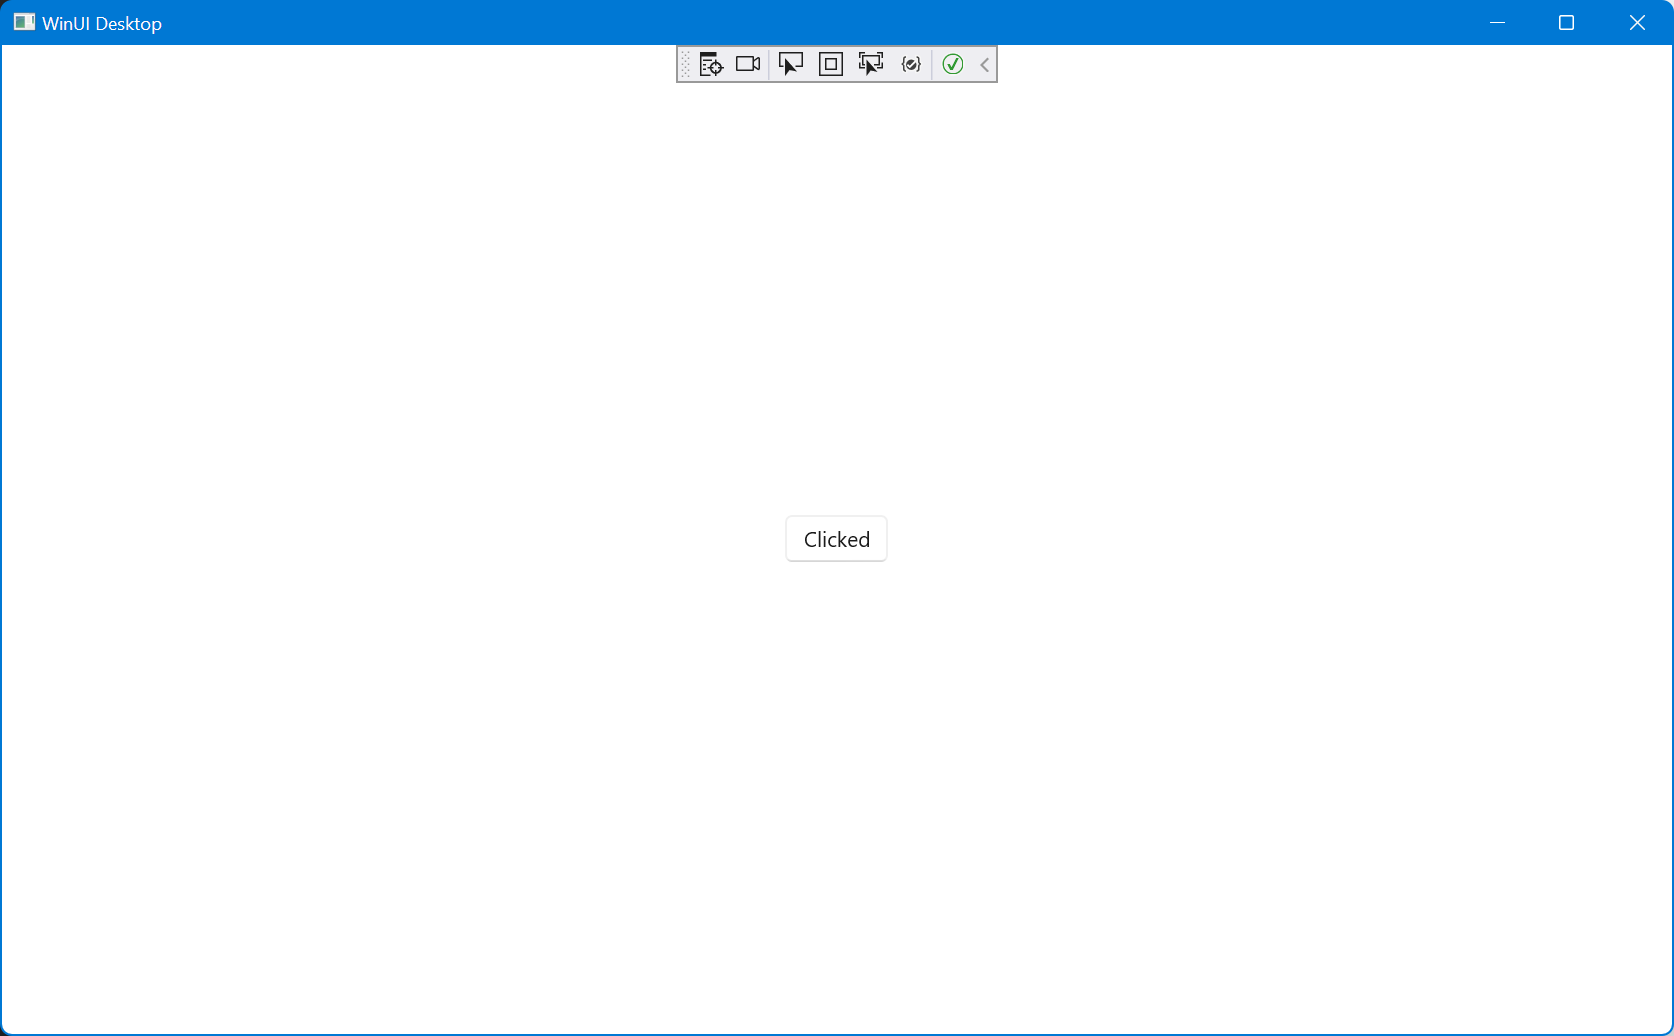
\includegraphics[width=\textwidth,height=\textheight,keepaspectratio]{Prototype-Button-Clicked.png}

\subsubsection{Testing and validation}

\begin{tabulary}{\linewidth}{|L|l|L|}
    \hline
    Test & Result & Remark \\
    \hline
    Does it compile & Pass & \\
    \hline
    Does it deploy & Pass & \\
    \hline
    Does it run & Pass & \\
    \hline
    Does the button work & Pass & \\
    \hline
\end{tabulary}

This is the simplest prototype, and its successful running means the development environment and the building tools are set up correctm, and I can start developing a more complex user interface.

\subsubsection{CI/CD pipeline}

I then set up the continuous integration pipeline based on the prototype. There are three jobs in the pipeline: test the app, build and sign the app, and deploy the app if a new version is released.

I am using the GitHub Actions\cite{github:actions} for this pipeline. I need to set up a YAML file to configure the pipeline.

\begin{minted}{yaml}
# The name of the pipeline
name: Build

# Triggered when a new commit is pushed to main
# Or a new tag is pushed to main
# Or a pull request is opened on main
on:
  push:
    branches: [main]
    tags:
      - '*'
  pull_request:
    branches: [main]

  workflow_dispatch:
  # Test the app using dotnet test
  test-app:
    name: Test App
    runs-on: windows-2022
    steps:
    - name: Checkout
      uses: actions/checkout@v2
      with:
        fetch-depth: 0
    
    # Cache nuget
    - uses: actions/cache@v2
      with:
        path: ~/.nuget/packages
        key: ${{ runner.os }}-nuget-${{ hashFiles('src\Algorithm Dynamics.Core\Algorithm Dynamics.Core.csproj') }}-${{ hashFiles('src\Algorithm Dynamics.Test\Algorithm Dynamics.Test.csproj') }}

    # Execute all unit tests in the solution
    - name: Execute unit tests
      working-directory: src\Algorithm Dynamics.Test
      run: dotnet test --filter TestCategory!=TestRunCode

  # Build the app using msbuild
  build-app:
    name: Build App
    runs-on: windows-2022
    env:
      Solution_Name: Algorithm Dynamics.sln
      Project_Directory: src\Algorithm Dynamics
    outputs:
      version: ${{ steps.getappmanifest.outputs.version }}
    strategy:
      matrix:
        targetPlatform: [x86, x64, arm64]
    steps:
    - name: Checkout
      uses: actions/checkout@v2
      with:
        fetch-depth: 0

    # Cache nuget
    - uses: actions/cache@v2
      with:
        path: ~/.nuget/packages
        key: ${{ runner.os }}-nuget-${{ matrix.targetplatform }}-${{ hashFiles('src\Algorithm Dynamics\Algorithm Dynamics.csproj') }}-${{ hashFiles('src\Algorithm Dynamics.Core\Algorithm Dynamics.Core.csproj') }}

    # Add MSBuild to the PATH: https://github.com/microsoft/setup-msbuild
    - name: Setup MSBuild.exe
      uses: microsoft/setup-msbuild@v1.1

    # Build app package
    - name: Create the ${{ matrix.targetplatform }} app package
      working-directory: src
      env:
        Solution_Name: Algorithm Dynamics.sln
        Appx_Bundle_Platforms: x86|x64|arm64
        Platform: ${{ matrix.targetplatform }}
        Configuration: Release
        Appx_Package_Build_Mode: StoreUpload
        Appx_Bundle: Never
        Appx_Package_Dir: AppPackages\
      run: |
        msbuild "$env:Solution_Name" /restore /p:AppxBundlePlatforms="$env:Appx_Bundle_Platforms" /p:Platform="$env:Platform" /p:Configuration=$env:Configuration /p:UapAppxPackageBuildMode=$env:Appx_Package_Build_Mode /p:AppxBundle=$env:Appx_Bundle /p:AppxPackageSigningEnabled=false /p:AppxPackageDir="$env:Appx_Package_Dir" /p:GenerateAppxPackageOnBuild=true -m

    # Upload build artifacts
    - name: Upload build artifacts
      uses: actions/upload-artifact@v2
      with:
        name: ${{ matrix.targetplatform }} Package
        path: src\Algorithm Dynamics\AppPackages\**\Algorithm Dynamics*.msix

    # Read the version of the app
    - name: Get app manifest
      id: getappmanifest
      working-directory: src
      run: |
        [xml]$manifest = get-content "Algorithm Dynamics\Package.appxmanifest"
        $version = $manifest.Package.Identity.Version
        echo $version
        echo "::set-output name=version::$version"

  # Sign the app
  sign-app:
    name: Sign App
    runs-on: windows-2022
    needs: [test-app, build-app]
    env:
      Solution_Name: Algorithm Dynamics.sln
      Project_Directory: src\Algorithm Dynamics
    steps:

    # Set up working directory
    - name: Create directory
      run: |
        mkdir src\Bundle
        mkdir "src\Algorithm Dynamics"

    # Decode the base 64 encoded pfx and save the Signing_Certificate
    - name: Decode the pfx
      id: decodepfx
      run: |
        $pfx_cert_byte = [System.Convert]::FromBase64String("${{ secrets.AlgorithmDynamics_TemporaryKey }}")
        $certificatePath = Join-Path -Path $env:Project_Directory -ChildPath AlgorithmDynamics_TemporaryKey.pfx
        [IO.File]::WriteAllBytes("$certificatePath", $pfx_cert_byte)
        echo "::set-output name=cert_path::$certificatePath"

    # Download build artifacts
    - name: Prepare x86 MSIX
      uses: actions/download-artifact@v2
      with:
        name: x86 Package
        path: src\Bundle

    - name: Prepare x64 MSIX
      uses: actions/download-artifact@v2
      with:
        name: x64 Package
        path: src\Bundle

    - name: Prepare arm64 MSIX
      uses: actions/download-artifact@v2
      with:
        name: arm64 Package
        path: src\Bundle

    # Bundle and sign the app
    - name: Create MSIX Bundle
      uses: LanceMcCarthy/Action-MsixBundler@v1.0.1
      with:
        msix-folder: src\Bundle
        msixbundle-filepath: src\Bundle\Algorithm Dynamics_x86_x64_arm64.msixbundle
        msixbundle-version: ${{ needs.build-app.outputs.version }}
        enable-bundle-signing: true
        certificate-path: ${{ steps.decodepfx.outputs.cert_path }}
        certificate-private-key: ${{ secrets.Pfx_Key }}

    # Remove the pfx
    - name: Remove the pfx
      run: |
        $certificatePath = Join-Path -Path $env:Project_Directory -ChildPath AlgorithmDynamics_TemporaryKey.pfx
        Remove-Item -path $certificatePath

    # Upload the MSIX package: https://github.com/marketplace/actions/upload-a-build-artifact
    - name: Upload build artifacts
      uses: actions/upload-artifact@v2
      with:
        name: MSIX Package Release
        path: src\Bundle\*.msixbundle

    - name: Delete Artifact
      uses: GeekyEggo/delete-artifact@v1.0.0
      with:
        name: |
          x86 Package
          x64 Package
          arm64 Package
        failOnError: false

  # Distribute to Microsoft Store
  distribute:
    if: startsWith(github.event.ref, 'refs/tags/v')
    name: Distribute App
    runs-on: [self-hosted]
    needs: [test-app, sign-app]
    steps:
      # Prepare the app
      - name: Prepare app
        uses: actions/download-artifact@v2
        with:
          name: MSIX Package Release
          path: Release
      
      # Publish to Microsoft Store
      - uses: isaacrlevin/windows-store-action@1.0
        name: Publish to Store
        with:
          tenant-id: ${{ secrets.AZURE_AD_TENANT_ID }}
          client-id: ${{ secrets.AZURE_AD_APPLICATION_CLIENT_ID }}
          client-secret: ${{ secrets.AZURE_AD_APPLICATION_SECRET }}
          app-id: ${{ secrets.STORE_APP_ID }}
          package-path: "Release"
          skip-polling: ""

\end{minted}

Now, everytime when I push a commit to the remote repo, the app will be automatically build and tested, which ensures the code quality throughout the developement stage.

Here is an example of a success run of the build job.

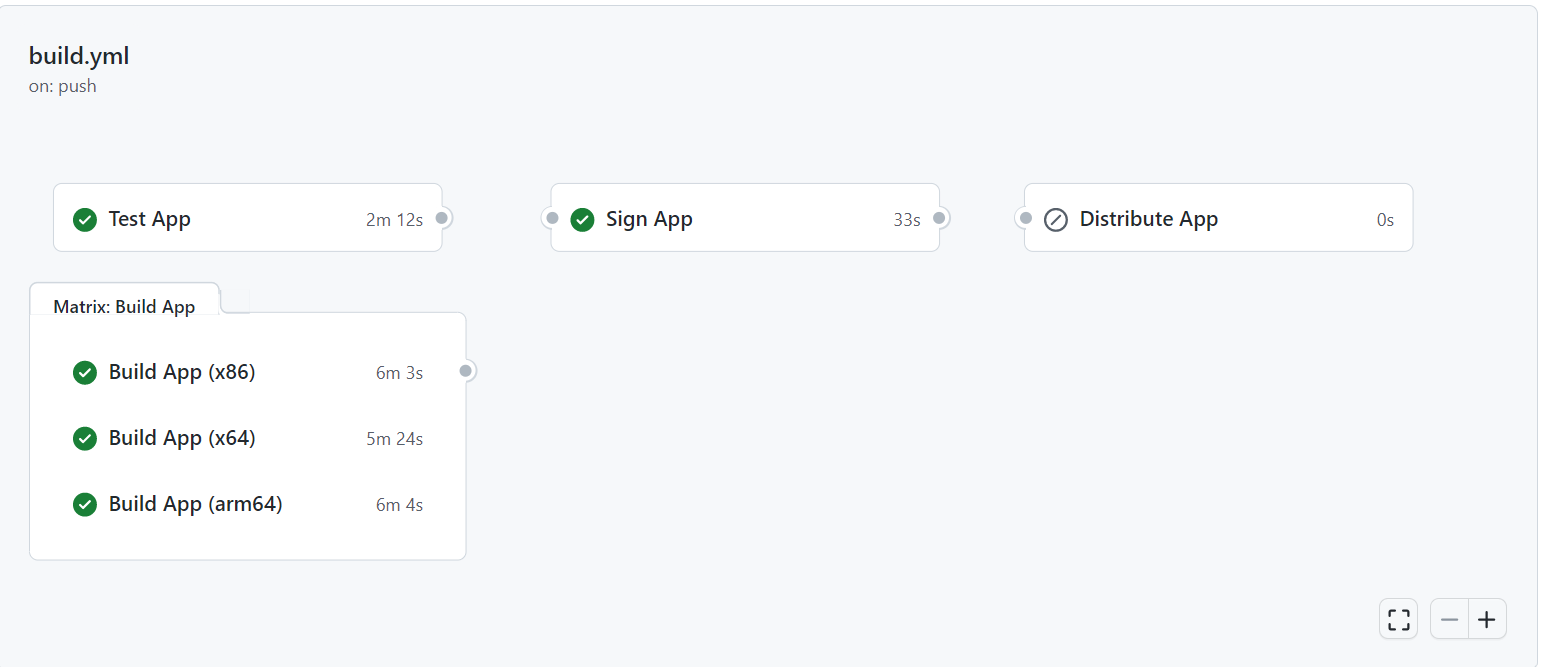
\includegraphics[width=\textwidth, height=\textheight, keepaspectratio]{CICD-Example}

\subsection{Create the NavigationView}

\subsubsection{Implementation}

First, I will implement the NavigationView as \hyperref[sec:NavigationViewDesign]{designed}. In the MainWindow.xaml file, I add the NavigationView control.

\begin{minted}{xml}
<NavigationView 
    x:Name="MainNavView"
    x:FieldModifier="public"
    IsBackButtonVisible="Collapsed"
    SelectionChanged="MainNavView_SelectionChanged">
</NavigationView>
\end{minted}

I assign a name \code{MainNavView} to the control so I can call it later in the code behind. I decide to hide the back button, which prevent the user to navigate the page in an unintended way. I also assign a \code{SelectionChanged} event handler to the control, which will be used to handle the navigation.

I then need to add different options to the navigation menu.

\begin{minted}{xml}
<NavigationView.MenuItems>
    <NavigationViewItem 
        x:Name="HomePageNavViewItem"
        Icon="Home"
        Content="Home"
        Tag="HomePage" />
    <NavigationViewItem
        x:Name="ProblemsPageNavViewItem"
        Icon="List"
        Content="Problems"
        Tag="ProblemsPage" />
    <NavigationViewItem
        x:Name="AssignmentsPageNavViewItem"
        Icon="Library"
        Content="Assignments"
        Tag="AssignmentsPage"/>
    <NavigationViewItem
        x:Name="PlaygroundPageNavViewItem"
        Icon="Edit"
        Content="Playground"
        Tag="PlaygroundPage"/>
</NavigationView.MenuItems>
\end{minted}

There are four options in the menu as designed. Each of which is assigned a name, icon, content and tag. The content and icon will be displayed to the user. The tag is used to identify the page that will be displayed when the option is clicked.

I add the account option to the footer.

\begin{minted}{xml}
<NavigationView.FooterMenuItems>
    <NavigationViewItem
        x:Name="AccountNavItem"
        Icon="Contact"
        Content="Account"
        Tag="AccountPage"/>
</NavigationView.FooterMenuItems>
\end{minted}

I add the content frame used to contain different pages.

\begin{minted}{xml}
<Frame
    x:Name="ContentFrame"
    Padding="0"
    Visibility="Visible"/>
\end{minted}

Now the layout of the NavigationView is finished. I need to add the code to initialize the control and handle the navigation.

When the main window is first initialized, the HomePage should be selected, and the title of the window should be set correctly. So I update the constructor of the main window to set the values.

\begin{minted}{csharp}
public MainWindow()
{
    InitializeComponent();
    Title = "Algorithm Dynamics";
    // Select HomePage when first loaded
    MainNavView.SelectedItem = MainNavView.MenuItems[0];
}
\end{minted}

Next, I need to handle the \code{SelectionChanged} event, this event gets triggered when the user clicks on a navigation item, and it will update the content frame to display the corresponding page.

\begin{minted}{csharp}
/// <summary>
/// Handle the SelectionChanged event of the MainNavView
/// Navigate to the corresponding page when the selection is changed
/// </summary>
/// <param name="sender"></param>
/// <param name="args"></param>
private void MainNavView_SelectionChanged(NavigationView sender, NavigationViewSelectionChangedEventArgs args)
{
    if (args.IsSettingsSelected)
    {
        // If the settings is selected, navigate to the settings page
        ContentFrame.Navigate(typeof(Pages.SettingsPage));
    }
    else
    {
        // Otherwise, get the selected item. If it is not null, get its Tag
        // Navigate to Algorithm_Dynamics.Pages.<Tag>
        NavigationViewItem selectedItem = args.SelectedItem as NavigationViewItem;
        if (selectedItem != null)
        {
            string tag = selectedItem.Tag as string;
            string pageName = "Algorithm_Dynamics.Pages." + tag;
            Type pageType = Type.GetType(pageName);
            ContentFrame.Navigate(pageType);
        }
    }
}
\end{minted}


Now, if I build and run the application, I should see the \code{NavigationView} works correctly. However, I get a runtime exception.

\begin{minted}{text}
System.NullReferenceException
  HResult=0x80004003
  Message=Object reference not set to an instance of an object.
  Source=WinRT.Runtime
  StackTrace:
   at ABI.System.Type.ToAbi(Type value)
   at ABI.System.Type.CreateMarshaler(Type value)
   at ABI.Microsoft.UI.Xaml.Controls.INavigate.global::Microsoft.UI.Xaml.Controls.INavigate.Navigate(Type sourcePageType)
   at Microsoft.UI.Xaml.Controls.Frame.Navigate(Type sourcePageType)
   at Algorithm_Dynamics.MainWindow.MainNavView_SelectionChanged(NavigationView sender, NavigationViewSelectionChangedEventArgs args) in C:\Algorithm-Dynamics\src\Algorithm Dynamics\MainWindow.xaml.cs:line 43
\end{minted}


It says object reference not set to an instance of an object when executing \code{ContentFrame.Navigate(pageType);}. This means the \code{pageType} does not exist. This is because I forget to create an actual HomePage, so it attempts to load a null object, failed, and throws the exception.

I create all pages under the \code{Algorithm_Dynamics.Pages} namespace. For now, all of them will only contain a text block showing their name. Here is an example of the HomePage.

\begin{minted}{xml}
<Page
    x:Class="Algorithm_Dynamics.Pages.HomePage"
    xmlns="http://schemas.microsoft.com/winfx/2006/xaml/presentation"
    xmlns:x="http://schemas.microsoft.com/winfx/2006/xaml"
    xmlns:local="using:Algorithm_Dynamics.Pages"
    xmlns:d="http://schemas.microsoft.com/expression/blend/2008"
    xmlns:mc="http://schemas.openxmlformats.org/markup-compatibility/2006"
    mc:Ignorable="d"
    Background="{ThemeResource ApplicationPageBackgroundThemeBrush}">

    <Grid>
        <TextBlock Text="HomePage"/>
    </Grid>
</Page>
\end{minted}


\begin{minted}{csharp}
using Microsoft.UI.Xaml.Controls;

namespace Algorithm_Dynamics.Pages
{
    public sealed partial class HomePage : Page
    {
        public HomePage()
        {
            this.InitializeComponent();
        }
    }
}
\end{minted}

Now, the software build and run successfully. The HomePage is correctly selected when it is launched and the TextBlock HomePage shows up correctly means that the right page is loaded.

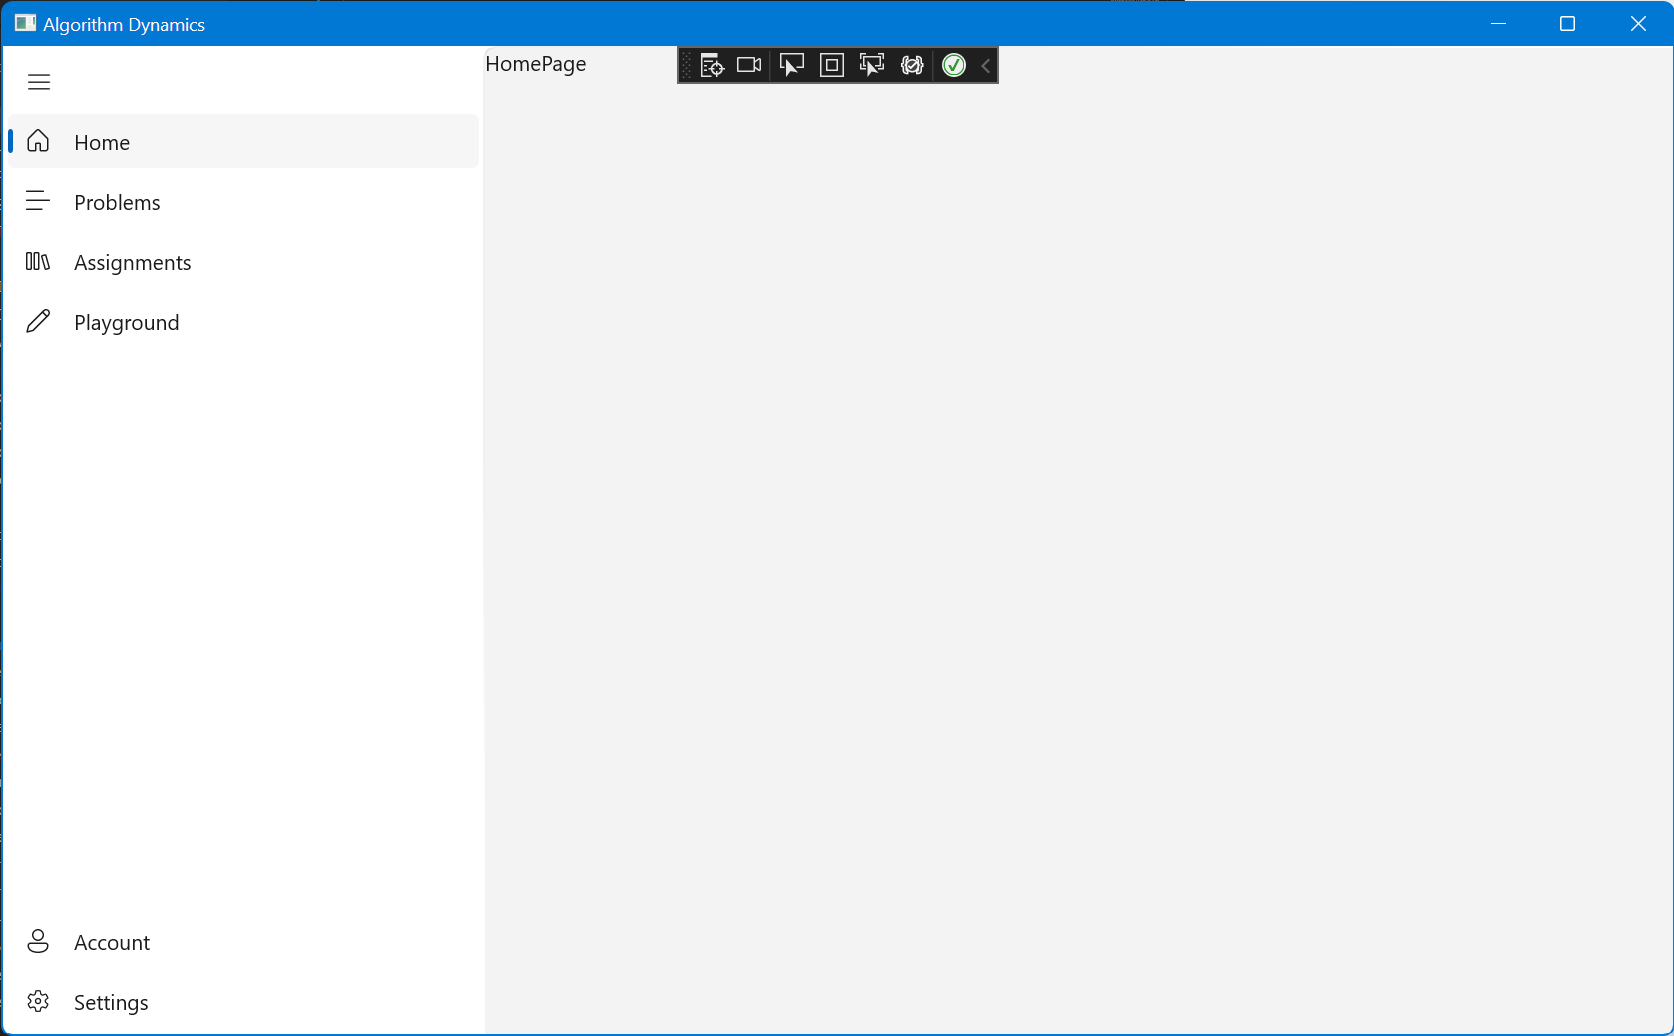
\includegraphics[width=\textwidth, height=\textheight, keepaspectratio]{HomePage-Draft-TextBlock}

When I click on other tabs on the NavigationView, the corresponding page is loaded correctly as well.

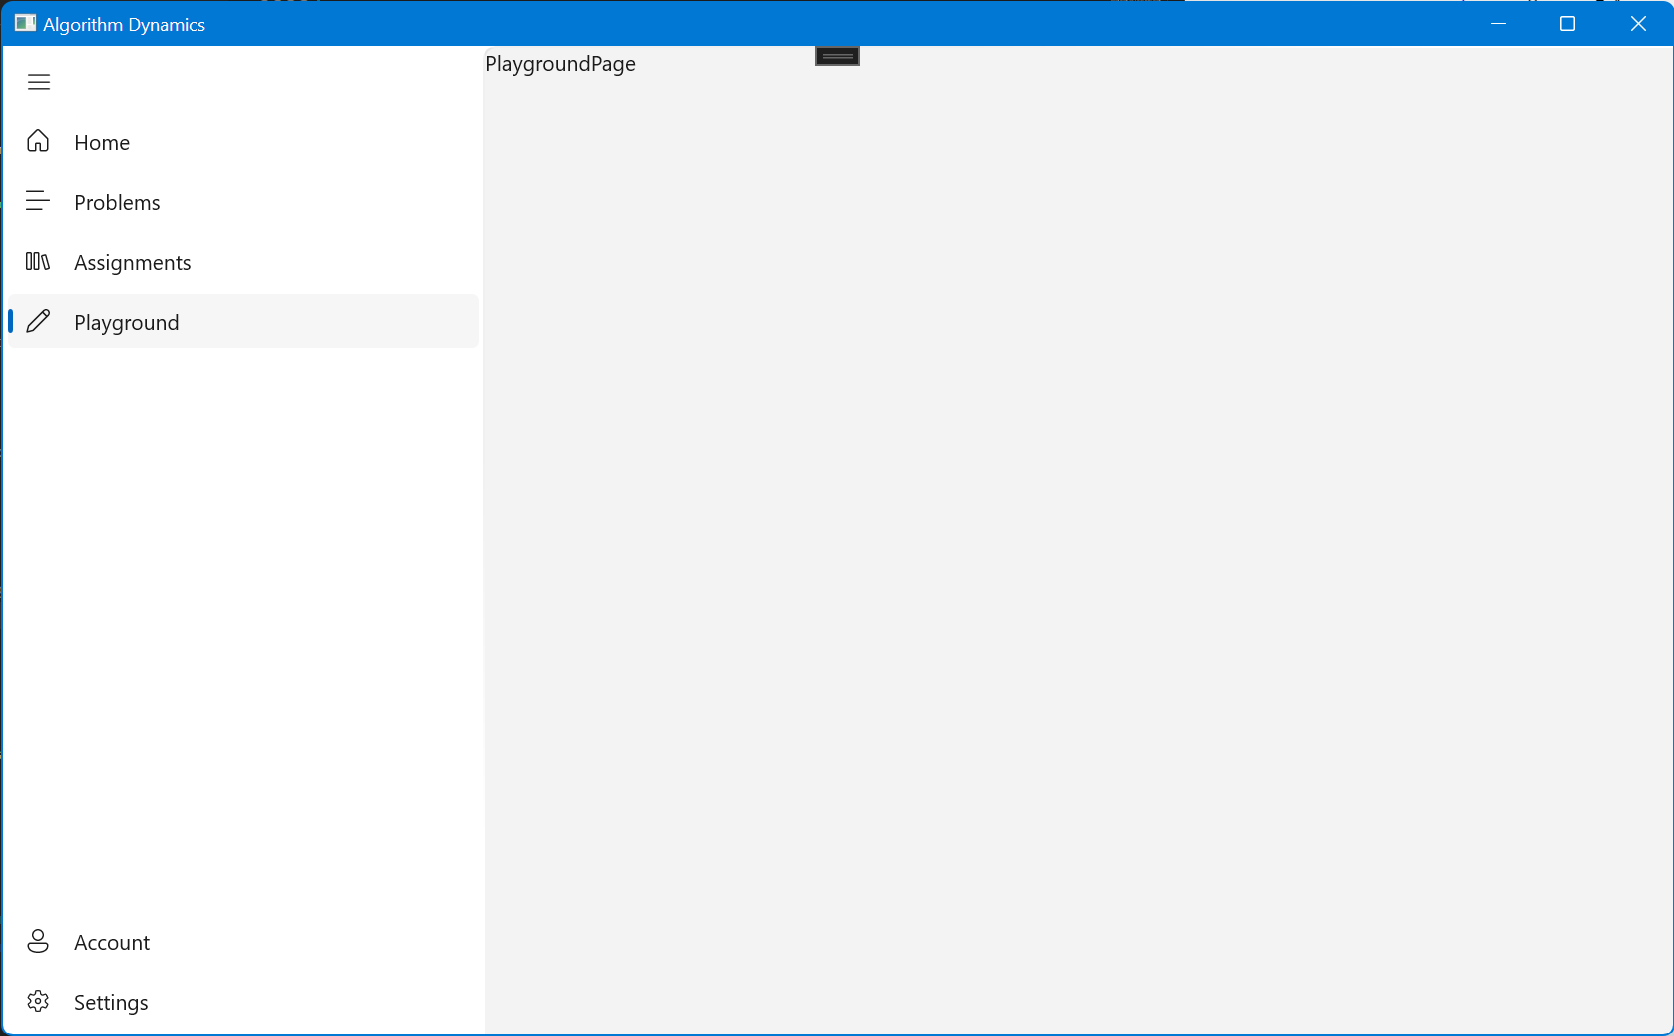
\includegraphics[width=\textwidth, height=\textheight, keepaspectratio]{PlaygroundPage-Draft-TextBlock}

\subsubsection{Testing and validation}

\begin{tabulary}{\linewidth}{|L|l|L|}
    \hline
    Test & Result & Remark \\
    \hline
    Does it load & Pass & \\
    \hline
    Does the button work & Pass & \\
    \hline
    Does it response to different screen size & Pass & \\
    \hline
\end{tabulary}

Now the NavigationView is built and tested. I will continue to build other components in the next section.

\subsection{Create the HomePage}

\subsubsection{Implementation}

The HomePage is made of three components, the background image, the quick access tools and the recommendations. They are wrapped by a scroller so they can be accessed on any size screen. I place a grid with two rows inside the \code{ScrollViewer}, the first row contains the background image, the second row contains the remaining tools.

\begin{minted}{xml}
<Page
    x:Class="Algorithm_Dynamics.Pages.HomePage"
    xmlns="http://schemas.microsoft.com/winfx/2006/xaml/presentation"
    xmlns:x="http://schemas.microsoft.com/winfx/2006/xaml"
    xmlns:local="using:Algorithm_Dynamics.Pages"
    xmlns:models="using:Algorithm_Dynamics.Models"
    xmlns:controls="using:CommunityToolkit.WinUI.UI.Controls"
    xmlns:d="http://schemas.microsoft.com/expression/blend/2008"
    xmlns:mc="http://schemas.openxmlformats.org/markup-compatibility/2006"
    mc:Ignorable="d"
    Background="{ThemeResource ApplicationPageBackgroundThemeBrush}">
    <ScrollViewer>
        <Grid>
            <Grid.RowDefinitions>
                <RowDefinition Height="auto"/>
                <RowDefinition Height="auto"/>
            </Grid.RowDefinitions>
            <Grid Grid.Row="0">
                <!-- Background Image -->
            </Grid>
            <Grid 
                Margin="24"
                Grid.Row="1">
                <!-- Quick Access tools and Recommendations -->
            </Grid>
        </Grid>
    </ScrollViewer>
</Page>
\end{minted}

Inside the background image grid, I place a \code{Image} control with the source of the background image. It is stretched to fill the entire grid so \code{Strecth} is set to \code{UniformToFill}.

\begin{minted}{xml}
<Image 
    Source="/Assets/HomePageBackgroundImage.jpg" 
    Height="256"
    Stretch="UniformToFill"/>
<TextBlock 
    Text="{x:Bind WelcomeMessage, Mode=OneTime, FallbackValue='Welcome User'}"
    HorizontalAlignment="Right"
    VerticalAlignment="Bottom"
    Margin="8"
    Foreground="White"
    Style="{ThemeResource TitleTextBlockStyle}"/>
\end{minted}

The \code{TextBlock} is used to display a greeting message. It is placed on the bottom right. Because its content needs to be adjusted by the current time and the current user, it is binded to the a variable \code{WelcomeMessage} so I can change its value programmatically.

\begin{minted}{csharp}
namespace Algorithm_Dynamics.Pages
{
    public sealed partial class HomePage : Page
    {
        /// <summary>
        /// The WelcomeMessage is displayed to the user on the HomePage
        /// </summary>
        public string WelcomeMessage { get; set; }
        public HomePage()
        {
            InitializeComponent();
        }
    }
}
\end{minted}

The welcome message is adjusted by different time in the day. It should also display the user name, but since the settings module is not implemented yet, I use a placeholder for the user name.

\begin{minted}{csharp}
/// <summary>
/// Set the WelcomeMessage based on the current time.
/// Morning: 00:00-12:00
/// Afternoon: 12:00-17:00
/// Evening 17:00-0:00
/// TODO Add the username after it is implemented
/// </summary>
private void SetWelcomeMessage()
{
    TimeSpan now = DateTime.Now.TimeOfDay;
    if (now >= new TimeSpan(00, 00, 00) && now < new TimeSpan(12, 00, 00))
    {
        WelcomeMessage = "Good morning, user!";
    }
    else if (now >= new TimeSpan(12, 00, 00) && now < new TimeSpan(17, 00, 00))
    {
        WelcomeMessage = "Good afternoon, user!";
    }
    else if (now >= new TimeSpan(17, 00, 00) && now <= new TimeSpan(23, 59, 59))
    {
        WelcomeMessage = "Good evening, user!";
    }
}
\end{minted}

Now I just need to set the welcome message in the constructor. Notice that it needs to be called before all components are initialized, so the text block can bind to the updated value.

\begin{minted}{csharp}
public HomePage()
{
    SetWelcomeMessage();
    InitializeComponent();
}
\end{minted}

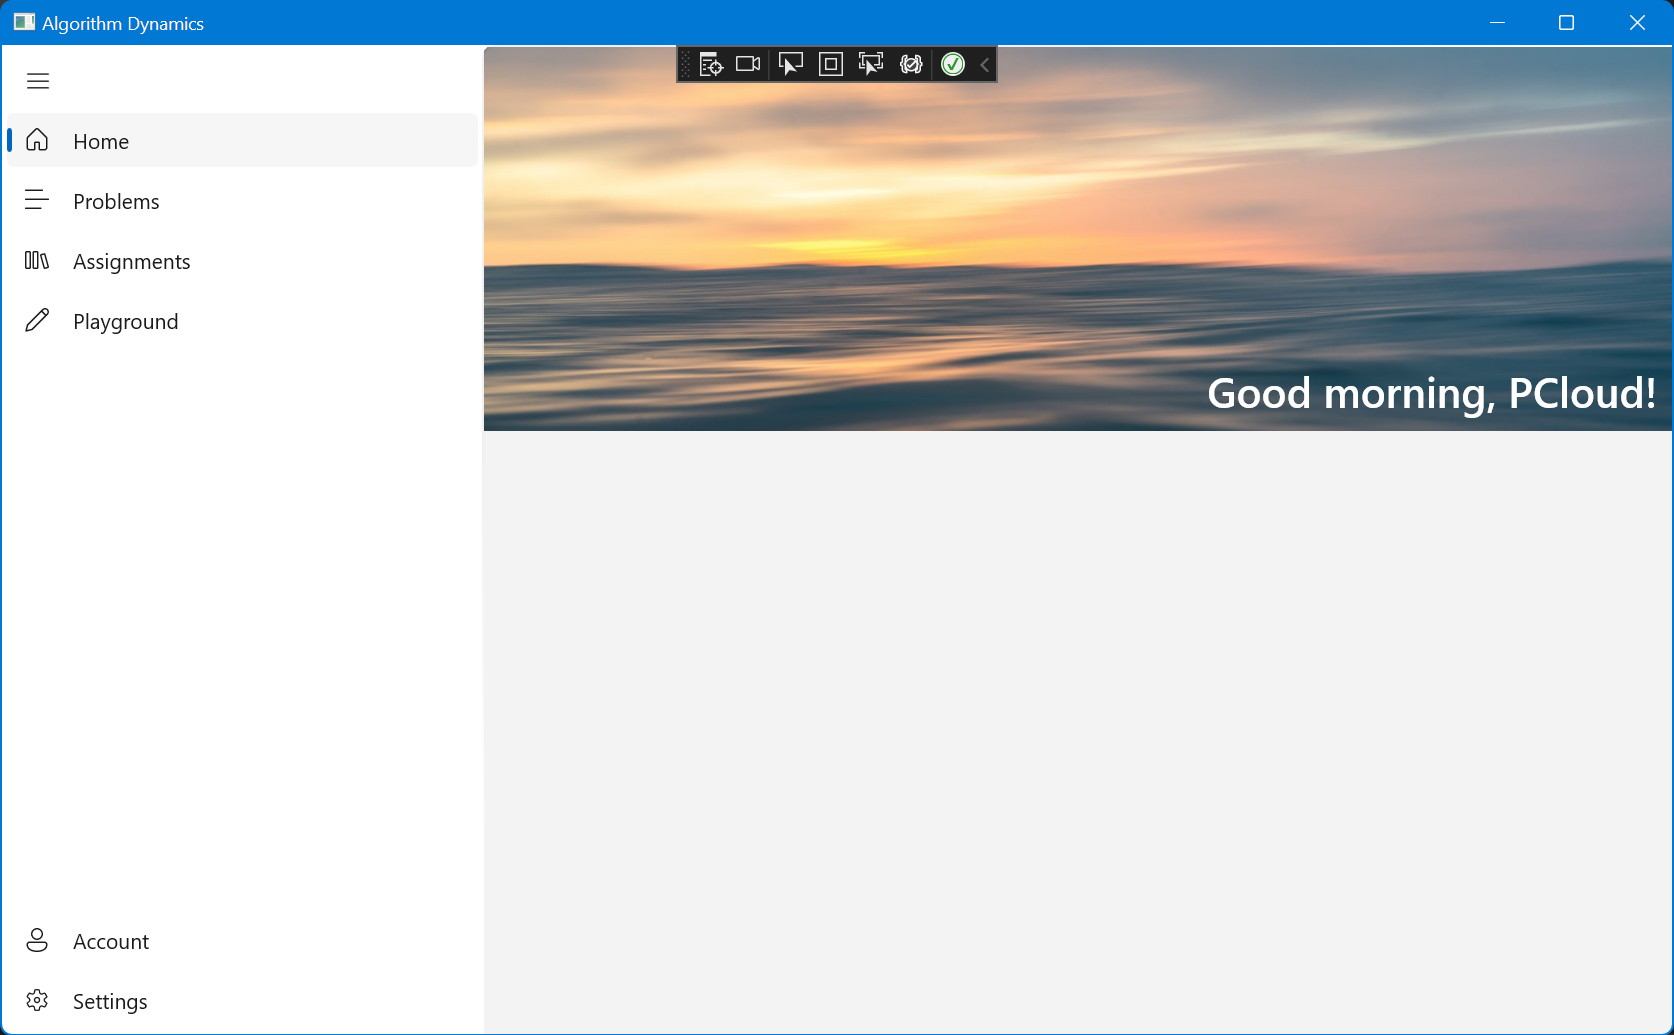
\includegraphics[width=\textwidth, height=\textheight, keepaspectratio]{HomePage-Image}

The image and the greeting message show up correctly, and because I am writing this in the morning, the correct greeting message is displayed.

For the quick access toolbar, I choose to use the \code{AdaptiveGridView} control for its \code{OneRowMode} function, which allows the toolbar to scroll horizontally on small screens. The controls in the quick access toolbar should be loaded dynamically, so they can be changed easily in the future. So I create a \code{QuickAccessItem} helper class. Each object will contain a name, an icon and an action. The name and the icon will be displayed to the user, and the action will be invoked when the user clicks on the control.

\begin{minted}{csharp}
using Microsoft.UI.Xaml.Controls;
using System;

namespace Algorithm_Dynamics.Models
{
    public class QuickAccessItem
    {
        public string Name { get; set; }
        public Symbol Icon { get; set; }
        public Action<MainWindow> Action { get; set; }
        public QuickAccessItem(string name, Symbol icon, Action<MainWindow> action)
        {
            Name = name;
            Icon = icon;
            Action = action;
        }
    }
}
\end{minted}

Then I create a \code{ObserableCollection} of \code{QAItems} that binds to the grid.

\begin{minted}{csharp}
public ObservableCollection<QuickAccessItem> QAItems { get; } = new ObservableCollection<QuickAccessItem>();
\end{minted}

\begin{minted}{xml}
<TextBlock 
    Text="Quick Access"
    Grid.Row="0"
    Style="{ThemeResource SubtitleTextBlockStyle}"/>
<controls:AdaptiveGridView 
    Grid.Row="1"
    Margin="4"
    ItemsSource="{x:Bind QAItems}"
    StretchContentForSingleRow="True"
    OneRowModeEnabled="True"
    ItemHeight="160"
    DesiredWidth="160"
    SelectionMode="None"
    IsItemClickEnabled="True">
    <GridView.ItemTemplate>
        <DataTemplate x:DataType="models:QuickAccessItem">
            <StackPanel 
                VerticalAlignment="Center"
                HorizontalAlignment="Center"
                Orientation="Vertical">
                <SymbolIcon 
                    x:Name="ItemIcon"
                    Symbol="{x:Bind Icon}"/>
                <TextBlock Text="{x:Bind Name}" />
            </StackPanel>
        </DataTemplate>
    </GridView.ItemTemplate>
</controls:AdaptiveGridView>
\end{minted}

I need to add the items to the collection when the HomePage is loaded. I create a procedure \code{InitializeQAItems}. Because I have passed the MainWindow object to the function, the MainNavView can be called inside. Because the CodingPage and the import/export logic is not completed yet, the Random Problem and Import function will be implemented later.

\begin{minted}{csharp}
public HomePage()
{
    SetWelcomeMessage();
    InitializeQAItems();
    InitializeComponent();
}
private void InitializeQAItems()
{
    QAItems.Clear();
    QAItems.Add(new QuickAccessItem("Random Problem", Symbol.Shuffle, (m_window) =>
    {
        m_window.MainNavView.SelectedItem = null;
        // TODO Navigate the ContentFrame to the Coding page manually
        throw new NotImplementedException("[Blocking]: The CodingPage has not been implemented yet.");
    }));
    QAItems.Add(new QuickAccessItem("Playground", Symbol.Edit, (m_window) =>
        m_window.MainNavView.SelectedItem = m_window.MainNavView.MenuItems[1]));
    QAItems.Add(new QuickAccessItem("Assignments", Symbol.Library, (m_window) =>
        m_window.MainNavView.SelectedItem = m_window.MainNavView.MenuItems[2]));
    QAItems.Add(new QuickAccessItem("Problems", Symbol.List, (m_window) =>
        m_window.MainNavView.SelectedItem = m_window.MainNavView.MenuItems[3]));
    QAItems.Add(new QuickAccessItem("Settings", Symbol.Setting, (m_window) =>
        m_window.MainNavView.SelectedItem = m_window.MainNavView.SettingsItem));
    QAItems.Add(new QuickAccessItem("Account", Symbol.Contact, (m_window) =>
        m_window.MainNavView.SelectedItem = m_window.MainNavView.FooterMenuItems[0]));
    QAItems.Add(new QuickAccessItem("Import", Symbol.Import, (m_window) =>
    {
        m_window.MainNavView.SelectedItem = null;
        // TODO Handle the import logic
        throw new NotImplementedException("[Blocking]: The import logic has not been implemented yet.");
    }));
}
\end{minted}

I need to handle the click event of the quick access toolbar. I create a procedure \code{QAGridView_ItemClick}, which will invoke the action of the item.

\begin{minted}{csharp}
/// <summary>
/// Handle the QAGridView click event. The Action will be invoked.
/// </summary>
/// <param name="sender"></param>
/// <param name="e"></param>
private void QAGridView_ItemClick(object sender, ItemClickEventArgs e)
{
    MainWindow m_window = (MainWindow)((App)Application.Current).m_window;
    if (e.ClickedItem is QuickAccessItem item)
    {
        item.Action(m_window);
    }
}
\end{minted}

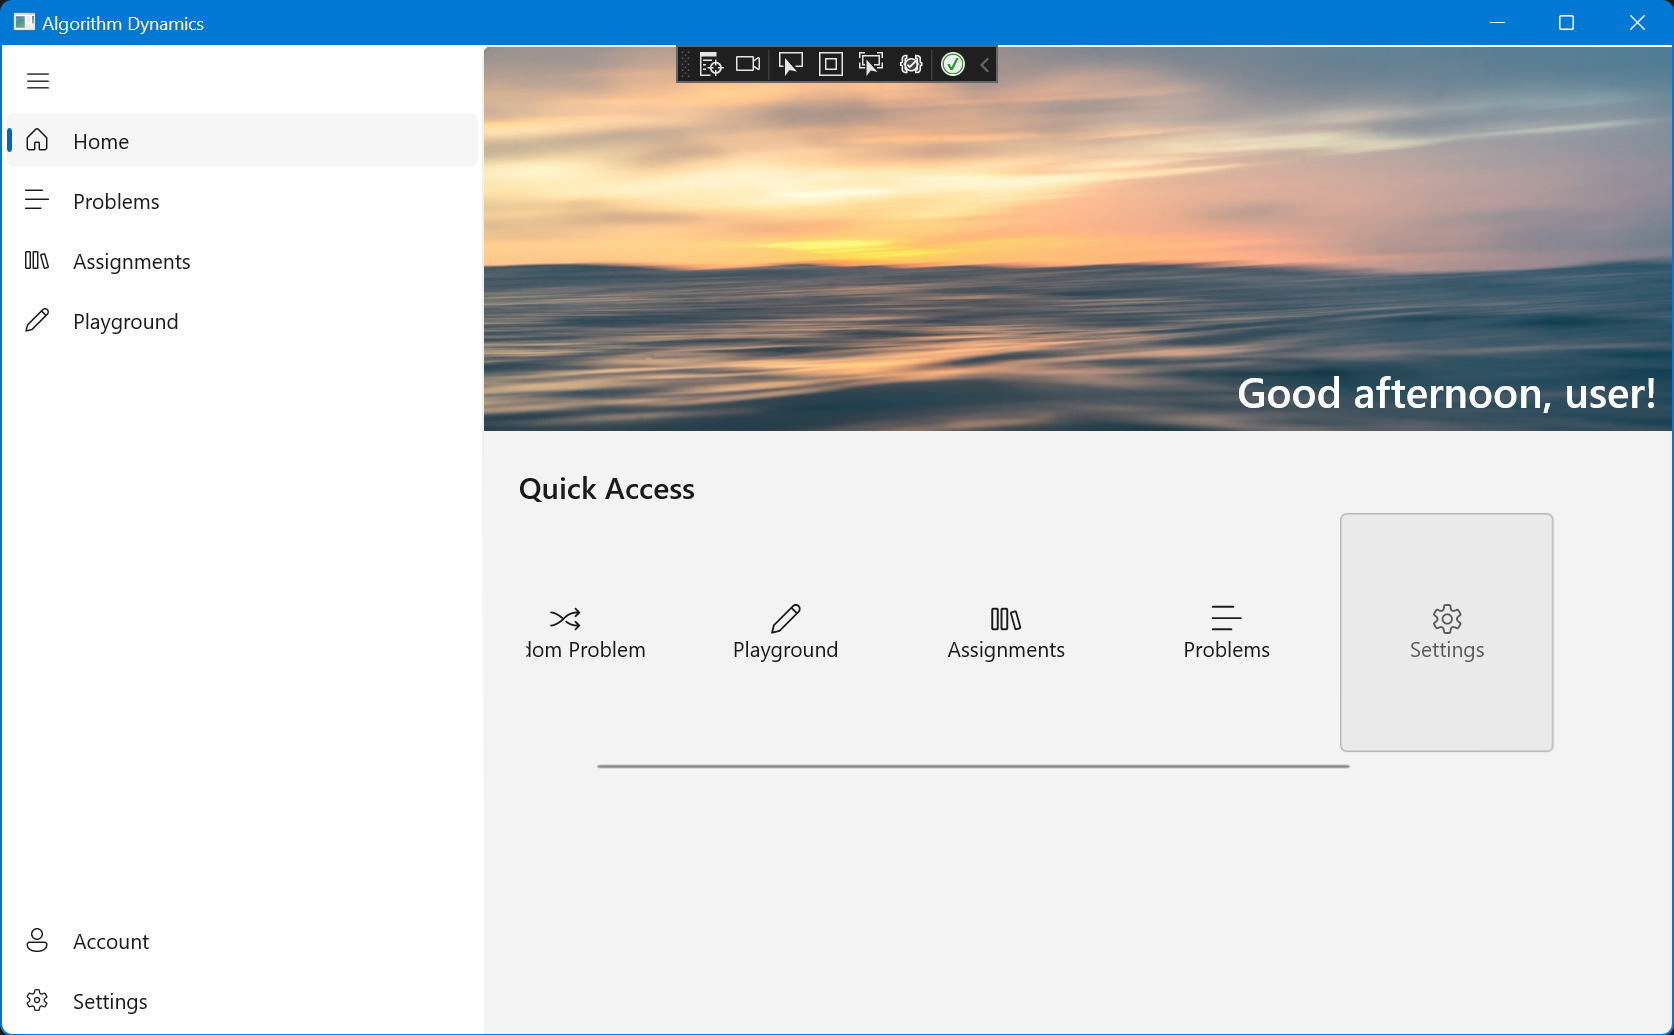
\includegraphics[width=\textwidth, height=\textheight, keepaspectratio]{HomePage-QuickAccessToolbar.png}

Now, when I build and run the application, the quick access toolbar shows up correctly and scroll horizontally as expected. When I click the different buttons, it navigates to the corresponding page correctly. When I click the Random Problem button, the software panic and a NotImplementedException is thrown with the correct error message.

\begin{minted}{text}
System.NotImplementedException
  HResult=0x80004001
  Message=[Blocking]: The CodingPage has not been implemented yet.
  Source=Algorithm Dynamics
  StackTrace:
   at Algorithm_Dynamics.Pages.HomePage.<>c.<InitializeQAItems>b__13_0(MainWindow m_window) in C:\Algorithm-Dynamics\src\Algorithm Dynamics\Pages\HomePage.xaml.cs:line 70
   at Algorithm_Dynamics.Pages.HomePage.QAGridView_ItemClick(Object sender, ItemClickEventArgs e) in C:\Algorithm-Dynamics\src\Algorithm Dynamics\Pages\HomePage.xaml.cs:line 59
   at WinRT._EventSource_global__Microsoft_UI_Xaml_Controls_ItemClickEventHandler.EventState.<GetEventInvoke>b__1_0(Object sender, ItemClickEventArgs e)
   at ABI.Microsoft.UI.Xaml.Controls.ItemClickEventHandler.<>c__DisplayClass10_0.<Do_Abi_Invoke>b__0(ItemClickEventHandler invoke)
   at ABI.Microsoft.UI.Xaml.Controls.ItemClickEventHandler.Do_Abi_Invoke(IntPtr thisPtr, IntPtr sender, IntPtr e)
\end{minted}

The recommendation control is similar. I create the \code{RecommendItem} class and add the items to the collection.

\begin{minted}{csharp}
namespace Algorithm_Dynamics.Models
{
    public class RecommendItem
    {
        public string Title { get; set; }
        public string Description { get; set; }
        public RecommendItem(string title, string description)
        {
            Title = title;
            Description = description;
        }
    }
}
\end{minted}

\begin{minted}{csharp}
public ObservableCollection<RecommendItem> RecItems { get; } = new ObservableCollection<RecommendItem>();
\end{minted}

Then bind the AdaptiveGridView to the collection.

\begin{minted}{csharp}
<TextBlock 
    Text="Recommended"
    Grid.Row="2"
    Style="{ThemeResource SubtitleTextBlockStyle}"/>
<controls:AdaptiveGridView
    x:Name="RecGridView"
    Grid.Row="3"
    Margin="4"
    ItemsSource="{x:Bind RecItems}"
    StretchContentForSingleRow="False"
    OneRowModeEnabled="False"
    ItemHeight="80"
    DesiredWidth="320"
    SelectionMode="None"
    IsItemClickEnabled="True"
    ItemClick="RecGridView_ItemClick">
    <GridView.ItemTemplate>
        <DataTemplate x:DataType="models:RecommendItem">
            <Grid HorizontalAlignment="Stretch">
                <StackPanel 
                    VerticalAlignment="Center"
                    HorizontalAlignment="Left"
                    Orientation="Vertical"
                    Margin="8">
                    <TextBlock Text="{x:Bind Title}"
                                Style="{ThemeResource BodyStrongTextBlockStyle}"/>
                    <TextBlock Text="{x:Bind Description}"/>
                </StackPanel>
            </Grid>
        </DataTemplate>
    </GridView.ItemTemplate>
</controls:AdaptiveGridView>
\end{minted}

For now, because the database and the data structure are not ready, I just add some dummy data to the collection. The recommendation logic will be added later.

\begin{minted}{csharp}
public HomePage()
{
    SetWelcomeMessage();
    InitializeQAItems();
    InitializeRecItems();
    InitializeComponent();
}
/// <summary>
/// TODO Generate Recommendation from database.
/// </summary>
private void InitializeRecItems()
{
    RecItems.Clear();
    RecItems.Add(new RecommendItem("Problem 1", "Easy | Data structure"));
    RecItems.Add(new RecommendItem("Problem 2", "Medium | Sorting"));
    RecItems.Add(new RecommendItem("Problem 3", "Hard | Graph"));
    RecItems.Add(new RecommendItem("Problem 4", "Easy | Data structure"));
    RecItems.Add(new RecommendItem("Assignment 1", "Due in 2 days"));
    RecItems.Add(new RecommendItem("Assignment 2", "Due in 3 days"));
    RecItems.Add(new RecommendItem("Assignment 3", "Due in 4 days"));
    RecItems.Add(new RecommendItem("Assignment 4", "Due in 5 days"));
}
\end{minted}

I need to handle the click event as well. And because neither the AssignmentsPage nor the CodingPage is ready, it will throw an NotImplementedException too.

\begin{minted}{csharp}
/// <summary>
/// Handle the RecGridView click event.
/// Navigate to the corresponding Problem or Assignment
/// </summary>
/// <param name="sender"></param>
/// <param name="e"></param>
private void RecGridView_ItemClick(object sender, ItemClickEventArgs e)
{
    // TODO Handle the navigation.
    throw new NotImplementedException("[Blocking]: The CodingPage or the AssignmentsPage has not been implemented yet.");
}
\end{minted}

Now, the HomePage is implemented. I run the application and test it.

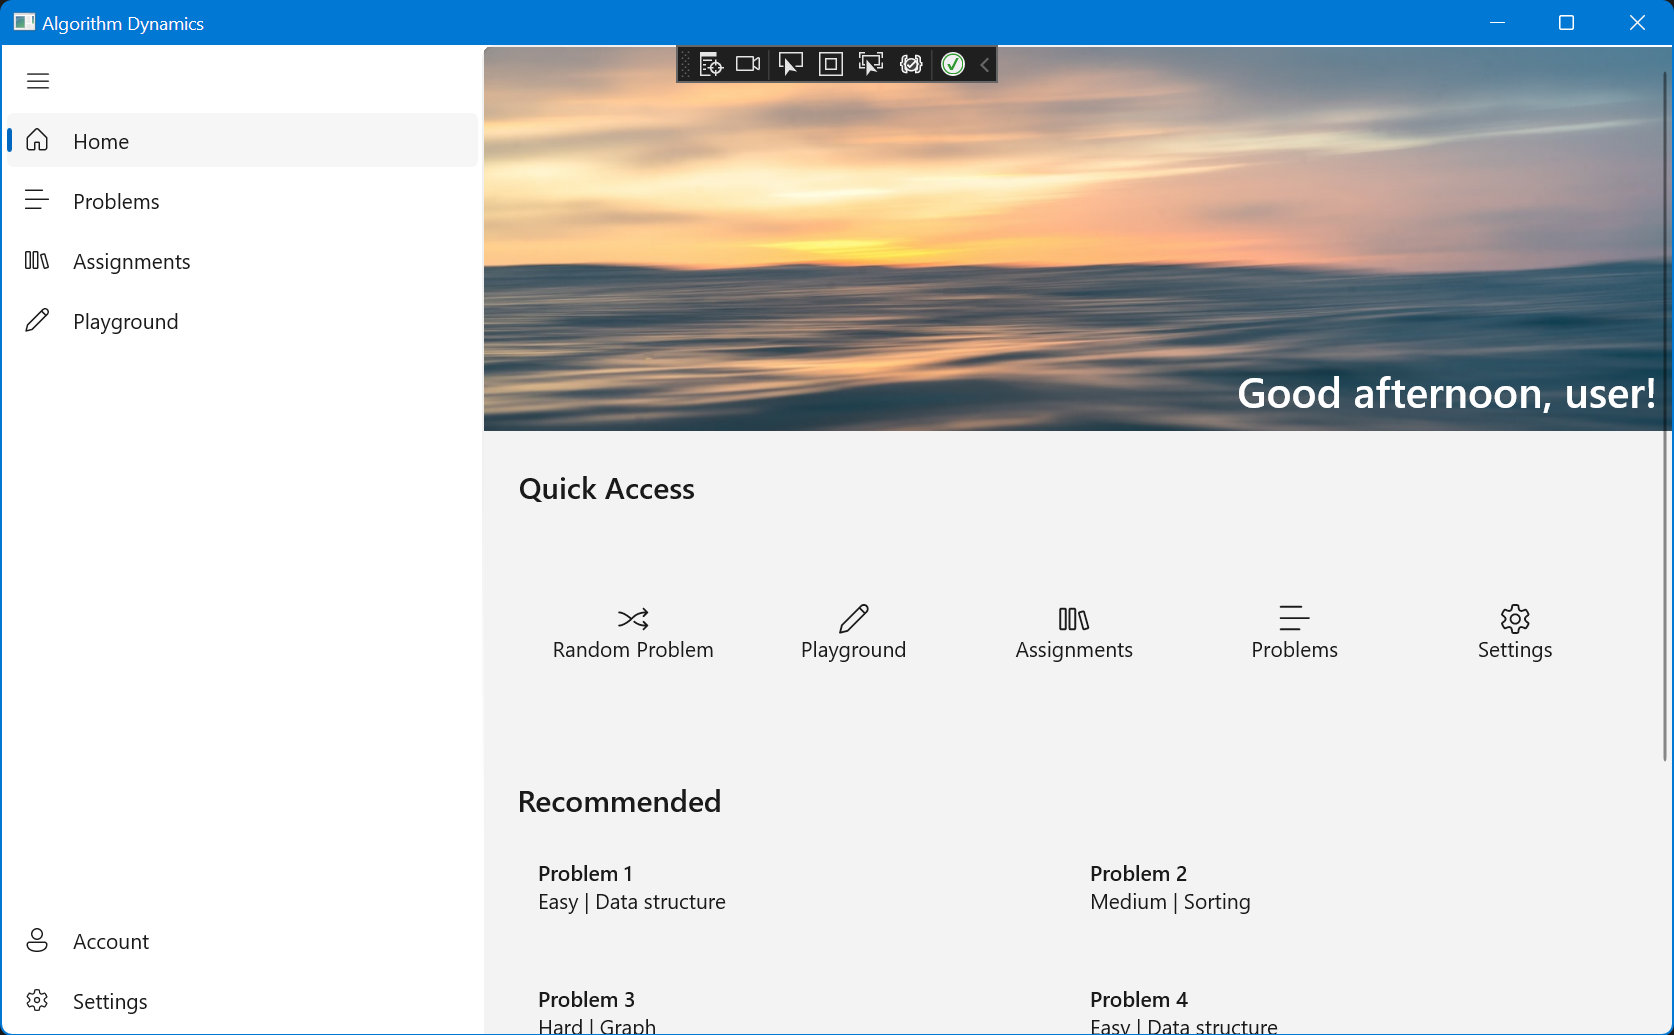
\includegraphics[width=\textwidth, height=\textheight, keepaspectratio]{HomePage-Finished}

All components show up correctly. The image is loaded and the greeting message is correct. The Quick Access Toolbar navigates correctly. When I click the recommended item, the correct exception is thrown.

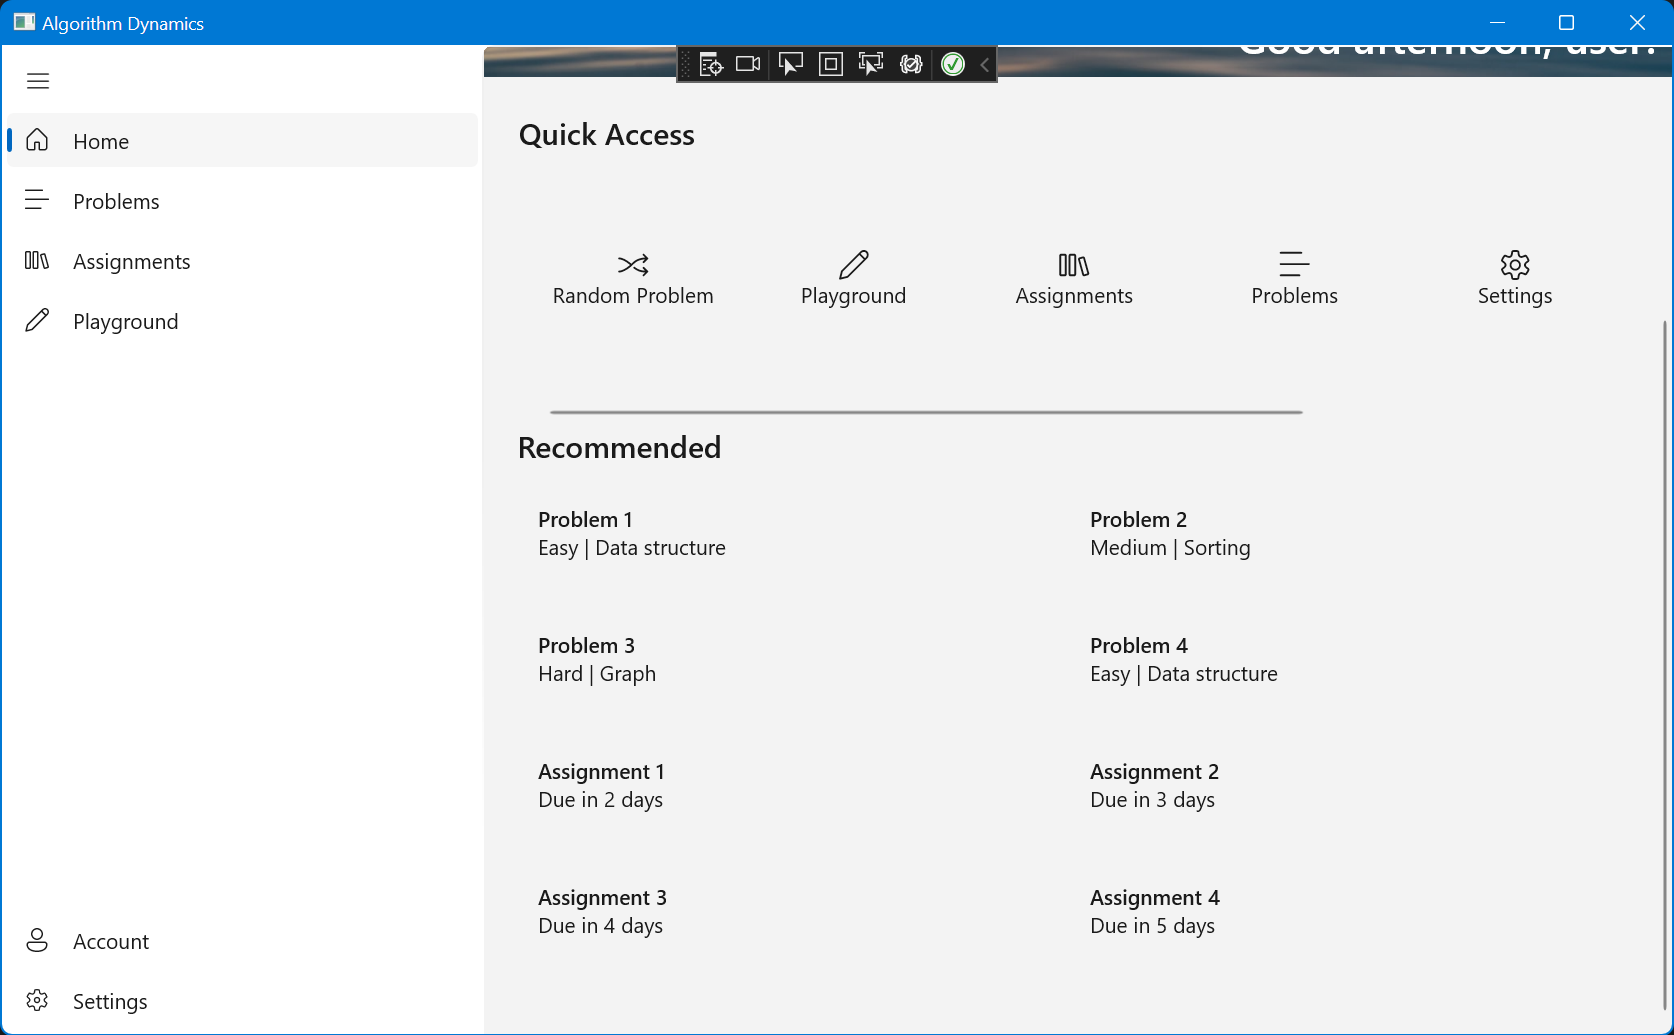
\includegraphics[width=\textwidth, height=\textheight, keepaspectratio]{HomePage-Finished-Scroll}

The scroller is working as well, so I can scroll down on a small window to see the recommendation items.

\subsubsection{Testing and validation}

\begin{tabulary}{\linewidth}{|L|l|L|}
    \hline
    Test & Result & Remark \\
    \hline
    Does it load & Pass & \\
    \hline
    Does the background image show up correctly & Pass & \\
    \hline
    Does the greeting message show up correctly & Pass & \\
    \hline
    Does the Quick Access Toolbar show up correctly & Pass & \\
    \hline
    Does the Quick Access Toolbar work correctly & Failed & The Random Problems and data import function is not implemented and will be implemented in the future. This test case will be reviewed then. \\
    \hline
    Does the Recommendation show up correctly & Pass &  \\
    \hline
    Does the Recommendation work correctly & Failed & The database and the data structure will be implemented in the future. This test case will be reviewed then. \\
    \hline
    Is the page responsive & Pass & \\
    \hline
\end{tabulary}

\subsection{Create the ProblemsPage}

\subsubsection{Implementation}

I move on to design the ProblemsPage. It contains two parts, the toolbar at the top and the problem list below. I will use a grid containing two rows to hold these two components.

\begin{minted}{xml}
<Page
    x:Class="Algorithm_Dynamics.Pages.ProblemsPage"
    xmlns="http://schemas.microsoft.com/winfx/2006/xaml/presentation"
    xmlns:x="http://schemas.microsoft.com/winfx/2006/xaml"
    xmlns:local="using:Algorithm_Dynamics.Pages"
    xmlns:d="http://schemas.microsoft.com/expression/blend/2008"
    xmlns:mc="http://schemas.openxmlformats.org/markup-compatibility/2006"
    mc:Ignorable="d"
    Background="{ThemeResource ApplicationPageBackgroundThemeBrush}">
    <Grid>
        <Grid.RowDefinitions>
            <RowDefinition Height="auto"/>
            <RowDefinition Height="*"/>
        </Grid.RowDefinitions>
        <Grid
            Grid.Row="0"
            HorizontalAlignment="Stretch">
            <!-- Toolbar -->
        </Grid>
        <Grid
            Grid.Row="1"
            HorizontalAlignment="Stretch">
            <!-- Problem List -->
        </Grid>
    </Grid>
</Page>
\end{minted}

For the toolbar, I use a grid with 6 columns to hold the search box and the ComboBoxes.

\begin{minted}{xml}
<Grid.ColumnDefinitions>
    <ColumnDefinition Width="2*"/>
    <ColumnDefinition Width="*"/>
    <ColumnDefinition Width="*"/>
    <ColumnDefinition Width="*"/>
    <ColumnDefinition Width="*"/>
    <ColumnDefinition Width="*"/>
</Grid.ColumnDefinitions>
<AutoSuggestBox 
    Grid.Column="0"
    Margin="4"
    PlaceholderText="Search..."
    x:Name="ProblemsSearchBox"
    HorizontalAlignment="Stretch"/>
<ComboBox 
    PlaceholderText="Difficulty"
    Grid.Column="1"
    Margin="4"
    ItemsSource="{x:Bind Difficulties}"
    HorizontalAlignment="Stretch"/>
<ComboBox 
    PlaceholderText="Status"
    Grid.Column="2"
    Margin="4"
    ItemsSource="{x:Bind Statuses}"
    HorizontalAlignment="Stretch"/>
<ComboBox 
    PlaceholderText="Tag"
    Grid.Column="3"
    Margin="4"
    ItemsSource="{x:Bind Tags}"
    HorizontalAlignment="Stretch"/>
<ComboBox 
    PlaceholderText="List"
    x:Name="ListComboBox"
    Grid.Column="4"
    Margin="4"
    ItemsSource="{x:Bind Lists}"
    HorizontalAlignment="Stretch"/>
<DropDownButton 
    Content="Add"
    Grid.Column="6"
    Margin="4"
    HorizontalAlignment="Stretch">
    <DropDownButton.Flyout>
        <MenuFlyout Placement="Bottom">
            <MenuFlyoutItem Text="New Problem"/>
            <MenuFlyoutItem Text="New Problem List"/>
            <MenuFlyoutItem Text="Import"/>
        </MenuFlyout>
    </DropDownButton.Flyout>
</DropDownButton>
\end{minted}

The ItemsSource of the ComboBox is binded to the corresponding variable, which allows me to set their value programmatically. Because the database is not implemented yet, I will use some dummy data to test the UI.

\begin{minted}{csharp}
using Microsoft.UI.Xaml.Controls;
using System.Collections.ObjectModel;

namespace Algorithm_Dynamics.Pages
{
    public sealed partial class ProblemsPage : Page
    {
        public ProblemsPage()
        {
            this.InitializeComponent();
        }
        private readonly ObservableCollection<string> Difficulties = new() { "Easy", "Medium", "Hard" };
        private readonly ObservableCollection<string> Statuses = new() { "Todo", "Attempted", "Done" };
        public ObservableCollection<string> Lists = new() { "List 1", "List 2", "List 3" };
        public ObservableCollection<string> Tags = new() { "Tag 1", "Tag 2", "Tag 3"};
    }
}
\end{minted}

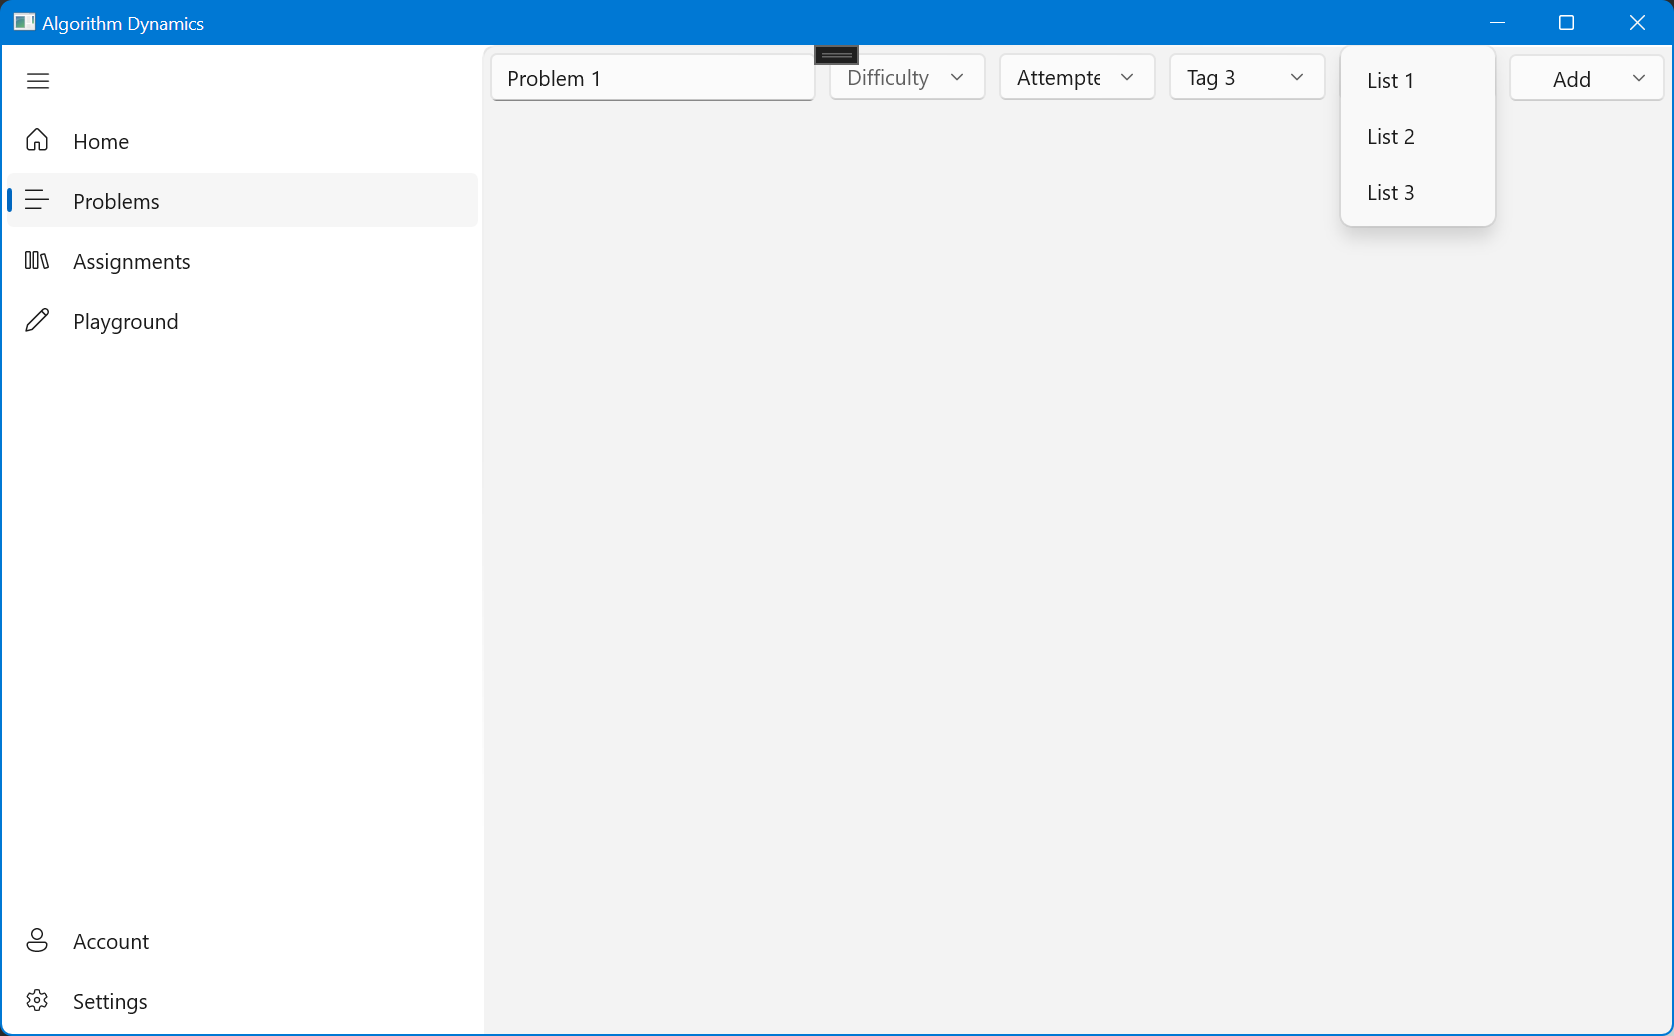
\includegraphics[width=\textwidth, height=\textheight, keepaspectratio]{ProblemsPage-Toolbar}

The toolbar shows up with all data loaded correctly. I can select an item correctly, but I cannot clear the selection. I need to empty the ComboBox when the user right clicks it. For the list ComboBox, I also need to allow the user to edit and delete an existing list, so when the user right click the list ComboBox, a menu flyout needs to show up with all options. I create a \code{ClearComboBox} procedure to handle the right click event.

\begin{minted}{csharp}
/// <summary>
/// Clear the <see cref="ComboBox"/>
/// </summary>
/// <param name="sender"></param>
/// <param name="e"></param>
private void ClearComboBox(object sender, RightTappedRoutedEventArgs e)
{
    ComboBox comboBox = (ComboBox)sender;
    comboBox.SelectedIndex = -1;
}
\end{minted}

And then bind the right clicked event to the procedure.

\begin{minted}{xml}
<ComboBox
    x:Name="DifficultyComboBox"
    RightTapped="ClearComboBox"/>
<ComboBox
    x:Name="StatusComboBox"
    RightTapped="ClearComboBox"/>
<ComboBox
    x:Name="TagComboBox"
    RightTapped="ClearComboBox"/>
\end{minted}

For the list ComboBox, I need to create the layout for the menu flyout first.

\begin{minted}{xml}
<ComboBox.Resources>
    <MenuFlyout x:Name="ListMenuFlyout">
        <MenuFlyout.Items>
            <MenuFlyoutItem 
                Text="Edit"
                Icon="Edit"/>
            <MenuFlyoutItem
                Text="Delete"
                Icon="Delete"/>
            <MenuFlyoutSeparator/>
            <MenuFlyoutItem
                Text="Clear"
                Icon="Clear"
                Click="ClearComboBox"/>
        </MenuFlyout.Items>
    </MenuFlyout>
</ComboBox.Resources>
\end{minted}

There are three items in the menu, edit, delete, and clear. The edit and delete function has not been implemented yet, so they will not be handled for now. Because the clear event is sent by the menu button instead of the ComboBox, I overload the \code{ClearComboBox} procedure to handle the clear event.

\begin{minted}{csharp}
/// <summary>
/// Clear the <see cref="ListComboBox"/>
/// </summary>
/// <param name="sender"></param>
/// <param name="e"></param>
private void ClearComboBox(object sender, RoutedEventArgs e)
{
    ListComboBox.SelectedIndex = -1;
}
\end{minted}

The menu flyout needs to be displayed when the list ComboBox is right clicked.

\begin{minted}{xml}
<ComboBox 
    x:Name="ListComboBox"
    RightTapped="ListComboBox_RightTapped">
\end{minted}

\begin{minted}{csharp}
/// <summary>
/// Display the <see cref="ListMenuFlyout"/> when the <see cref="ListComboBox"/> is right tapped
/// </summary>
/// <param name="sender"></param>
/// <param name="e"></param>
private void ListComboBox_RightTapped(object sender, RightTappedRoutedEventArgs e)
{
    ComboBox comboBox = (ComboBox)sender;
    ListMenuFlyout.ShowAt(comboBox, e.GetPosition(comboBox));
}
\end{minted}

Now, I build and run the code again. When I right-click the difficulty, status and tag ComboBox, their content is cleared correctly. When I click the list ComboBox, the menu flyout shows up. When I click the clear option, the selected list is cleared correctly. When I right-click other ComboBoxes, the content is cleared correctly as well.

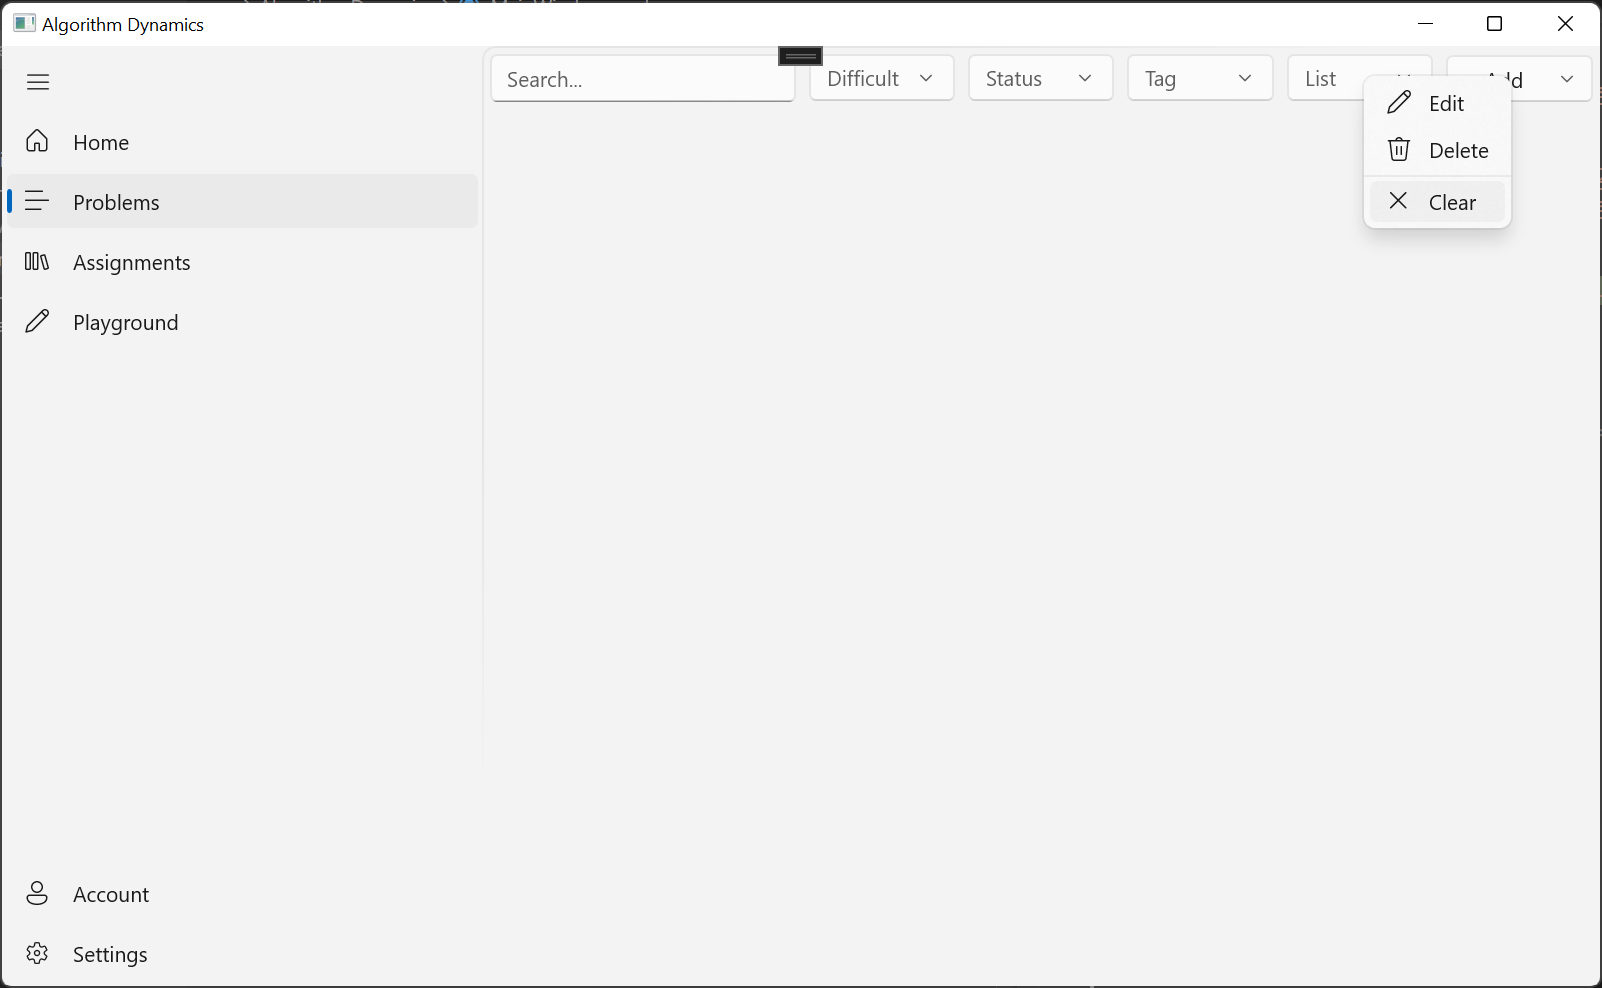
\includegraphics[width=\textwidth, height=\textheight, keepaspectratio]{ProblemsPage-ListComboBox-FlyoutMenu}

But there is a potential issue with the current implementation. When I right-click the list ComboBox, the menu flyout will show up even when no list is selected. Clear the box does not result in any problem because it is empty anyway, but in the future, when the edit and delete function is implemented, attempting to edit or delete an empty list will cause a problem. So I need to change the logic of the menu flyout so that it only shows up when there is something selected. I only need to modify the original function, and only show the flyout when the selected index is -1.

\begin{minted}{csharp}
private void ListComboBox_RightTapped(object sender, RightTappedRoutedEventArgs e)
{
    ComboBox comboBox = (ComboBox)sender;
    if (comboBox.SelectedIndex != -1)
    {
        ListMenuFlyout.ShowAt(comboBox, e.GetPosition(comboBox));
    }
}
\end{minted}

Now, the menu flyout does not show up when no list is selected, which fixes a potential issue in the future.

Next, I need to handle the delete and edit event for the list ComboBox. Because the actual database and data structures have not been implemented yet, I will only create the UI for these events and implement their functions later. For the edit event, the content frame should navigate to the edit page. For the delete event, a content dialog will show up to confirm the deletion. I create two procedures to handle these events.

\begin{minted}{csharp}
/// <summary>
/// Navigate to the edit ProblemList page
/// </summary>
/// <param name="sender"></param>
/// <param name="e"></param>
/// <exception cref="NotImplementedException"></exception>
private void EditProblemList(object sender, RoutedEventArgs e)
{
    // TODO Navigate to edit page
    throw new NotImplementedException();
}

/// <summary>
/// Show a content dialog to confirm the deletion of a ProblemList
/// </summary>
/// <param name="sender"></param>
/// <param name="e"></param>
/// <exception cref="NotImplementedException"></exception>
private async void DeleteProblemList(object sender, RoutedEventArgs e)
{
    ContentDialog dialog = new ContentDialog();
    dialog.Title = "Delete Problem List";
    dialog.PrimaryButtonText = "Delete";
    dialog.CloseButtonText = "Cancel";
    dialog.Content = $"Are you sure that you want to permanently delete {ListComboBox.SelectedItem}?";
    dialog.DefaultButton = ContentDialogButton.Close;
    dialog.XamlRoot = this.Content.XamlRoot;
    var result = await dialog.ShowAsync();
    if (result == ContentDialogResult.Primary)
    {
        // TODO Delete the selected problem list
        throw new NotImplementedException();
    }
}
\end{minted}

Now, when I click the delete button, a popup shows up correctly to confirm deletion.

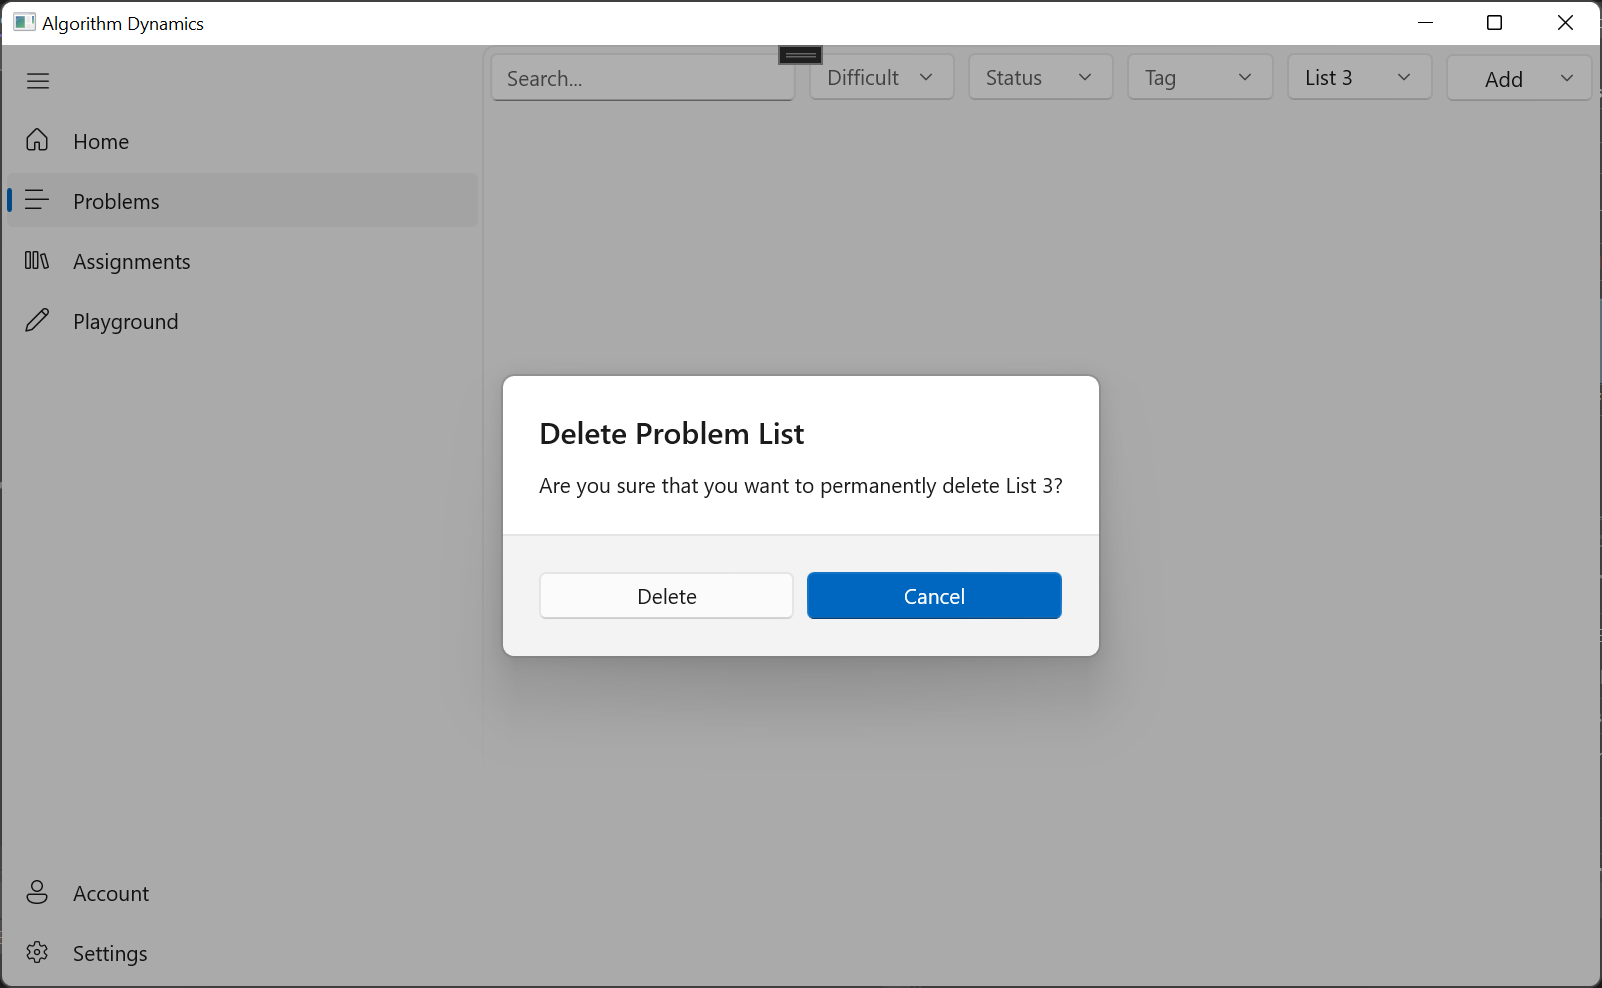
\includegraphics[width=\textwidth, height=\textheight, keepaspectratio]{ProblemsPage-ContentDialog}

I then implement the problem list below the toolbar. I use a \code{ListView} to display the problem list. Similarly, I bind the data source to a variable Problems which contains a list of Problem. For each problem, its name, difficulty, status and tags are displayed.

\begin{minted}{xml}
<ListView x:Name="ProblemsListView"
    Grid.Row="1"
    SelectionMode="Extended"
    Width="auto"
    ItemsSource="{x:Bind Problems, Mode=OneWay}">
    <ListView.ItemContainerStyle>
        <Style TargetType="ListViewItem">
            <Setter Property="HorizontalContentAlignment" Value="Stretch"/>
        </Style>
    </ListView.ItemContainerStyle>
    <ListView.ItemTemplate>
        <DataTemplate x:DataType="local:Problem">
            <Grid>
                <Grid.ColumnDefinitions>
                    <ColumnDefinition Width="2*"/>
                    <ColumnDefinition Width="*"/>
                    <ColumnDefinition Width="*"/>
                    <ColumnDefinition Width="2*"/>
                    <ColumnDefinition Width="*"/>
                </Grid.ColumnDefinitions>
                <TextBlock
                    Text="{x:Bind Name}"
                    Grid.Column="0"
                    HorizontalAlignment="Left"
                    VerticalAlignment="Center"
                    Margin="4 0 0 0"/>
                <TextBlock
                    Text="{x:Bind Difficulty}"
                    Grid.Column="1"
                    HorizontalAlignment="Left"
                    VerticalAlignment="Center"
                    Margin="10 0 0 0"/>
                <TextBlock
                    Text="{x:Bind Status}"
                    Grid.Column="2"
                    HorizontalAlignment="Left"
                    VerticalAlignment="Center"
                    Margin="14 0 0 0"/>
                <TextBlock
                    Text="{x:Bind Tags}"
                    Grid.Column="3"
                    HorizontalAlignment="Left"
                    VerticalAlignment="Center"
                    TextTrimming="CharacterEllipsis"
                    Margin="17 0 0 0"/>
                <Button
                    Content="Start"
                    Grid.Column="4"
                    HorizontalAlignment="Stretch"
                    Margin="12 0 0 0"/>
            </Grid>
        </DataTemplate>
    </ListView.ItemTemplate>
</ListView>
\end{minted}

Because the data structure for Problem has not been implemented yet, I create a sample class for the Problem. It only contains the four attributes that matters and a constructor to initialize the values.

\begin{minted}{csharp}
public class Problem
{
    public Problem(string name, string difficulty, string status, string tags)
    {
        Name = name;
        Difficulty = difficulty;
        Status = status;
        Tags = tags;
    }

    public string Name { get; set; }
    public string Difficulty { get; set; }
    public string Status { get; set; }
    public string Tags { get; set; }
}
\end{minted}

I create a ObserableCollection for the list of Problem and add some sample data to it.

\begin{minted}{csharp}
public ObservableCollection<Problem> Problems = new();
public ProblemsPage()
{
    InitializeComponent();
    Problems.Add(new Problem("Problem 1", "Easy", "Todo", "Tag"));
    Problems.Add(new Problem("Problem 2", "Easy", "Attempted", "Tag"));
    Problems.Add(new Problem("Problem 3", "Easy", "Done", "Tag"));
    Problems.Add(new Problem("Problem 4", "Medium", "Todo", "Tag"));
    Problems.Add(new Problem("Problem 5", "Medium", "Attempted", "Tag"));
    Problems.Add(new Problem("Problem 6", "Medium", "Done", "Tag"));
    Problems.Add(new Problem("Problem 7", "Hard", "Todo", "Tag"));
    Problems.Add(new Problem("Problem 8", "Hard", "Attempted", "Tag"));
    Problems.Add(new Problem("Problem 9", "Hard", "Done", "Tag"));
    Problems.Add(new Problem("Problem 10", "Hard", "Todo", "Tag"));
}
\end{minted}

The problem list shows up with the correct data.

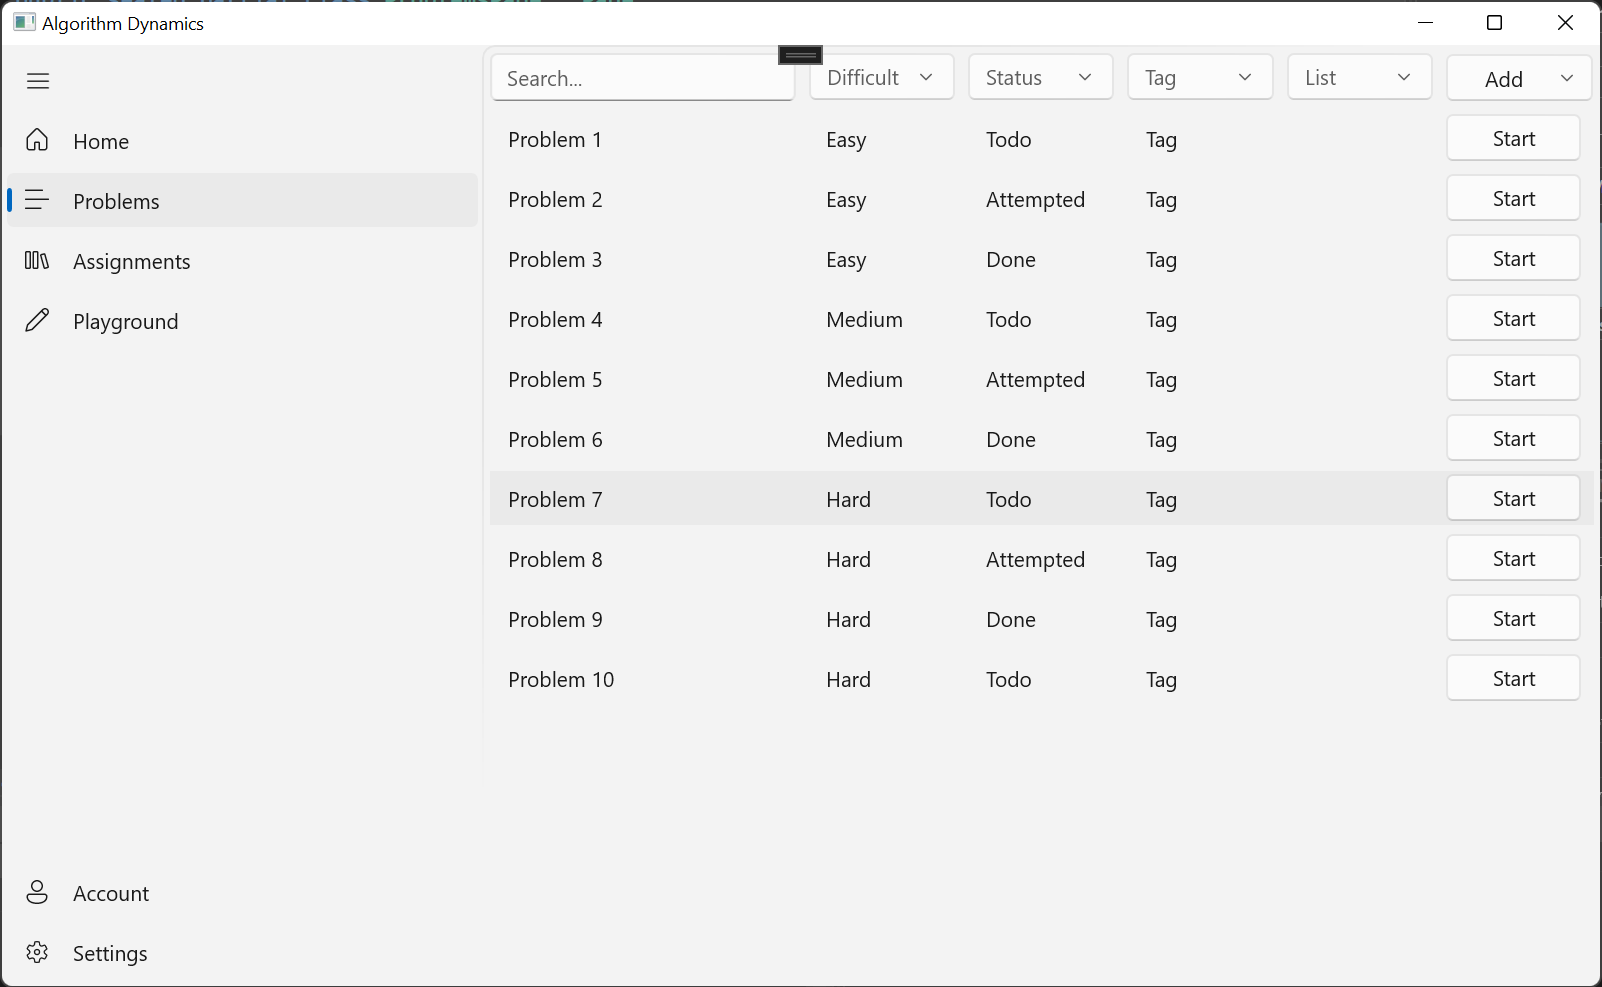
\includegraphics[width=\textwidth, height=\textheight, keepaspectratio]{ProblemsPage-ProblemList}

I need to add a flyout menu for the problem list to allow the user to edit and delete problems when right clicking the list. When only one problem is selected, the user can edit it or delete it. When multiple problems are selected, the user can delete all of them or create a problem list from them.

\begin{minted}{xml}
<ListView.Resources>
    <MenuFlyout x:Name="SingleSelectedMenuFlyout">
        <MenuFlyout.Items>
            <MenuFlyoutItem 
                Text="Edit"
                Icon="Edit"/>
            <MenuFlyoutItem 
                Text="Delete"
                Icon="Delete"/>
        </MenuFlyout.Items>
    </MenuFlyout>
    <MenuFlyout x:Name="MultipleSelectedMenuFlyout">
        <MenuFlyout.Items>
            <MenuFlyoutItem 
                Text="Create Problem List..."
                Icon="Add"/>
            <MenuFlyoutItem 
                Text="Delete"
                Icon="Delete"/>
        </MenuFlyout.Items>
    </MenuFlyout>
</ListView.Resources>
\end{minted}


\begin{minted}{csharp}
/// <summary>
/// Show flyout when the user right tapped the ProblemListView
/// When one problem is selected, show the SingleSelectedMenuFlyout
/// When mutiple problems are selected, show the MultipleSelectedMenuFlyout
/// </summary>
/// <param name="sender"></param>
/// <param name="e"></param>
private void ProblemsListView_RightTapped(object sender, RightTappedRoutedEventArgs e)
{
    ListView listView = (ListView)sender;
    if (listView.SelectedItems.Count == 1)
    {
        SingleSelectedMenuFlyout.ShowAt(listView, e.GetPosition(listView));
    }
    else if (listView.SelectedItems.Count > 1)
    {
        MultipleSelectedMenuFlyout.ShowAt(listView, e.GetPosition(listView));
    }
}
\end{minted}

The corresponding menu flyout can show up correctly based on the selection.

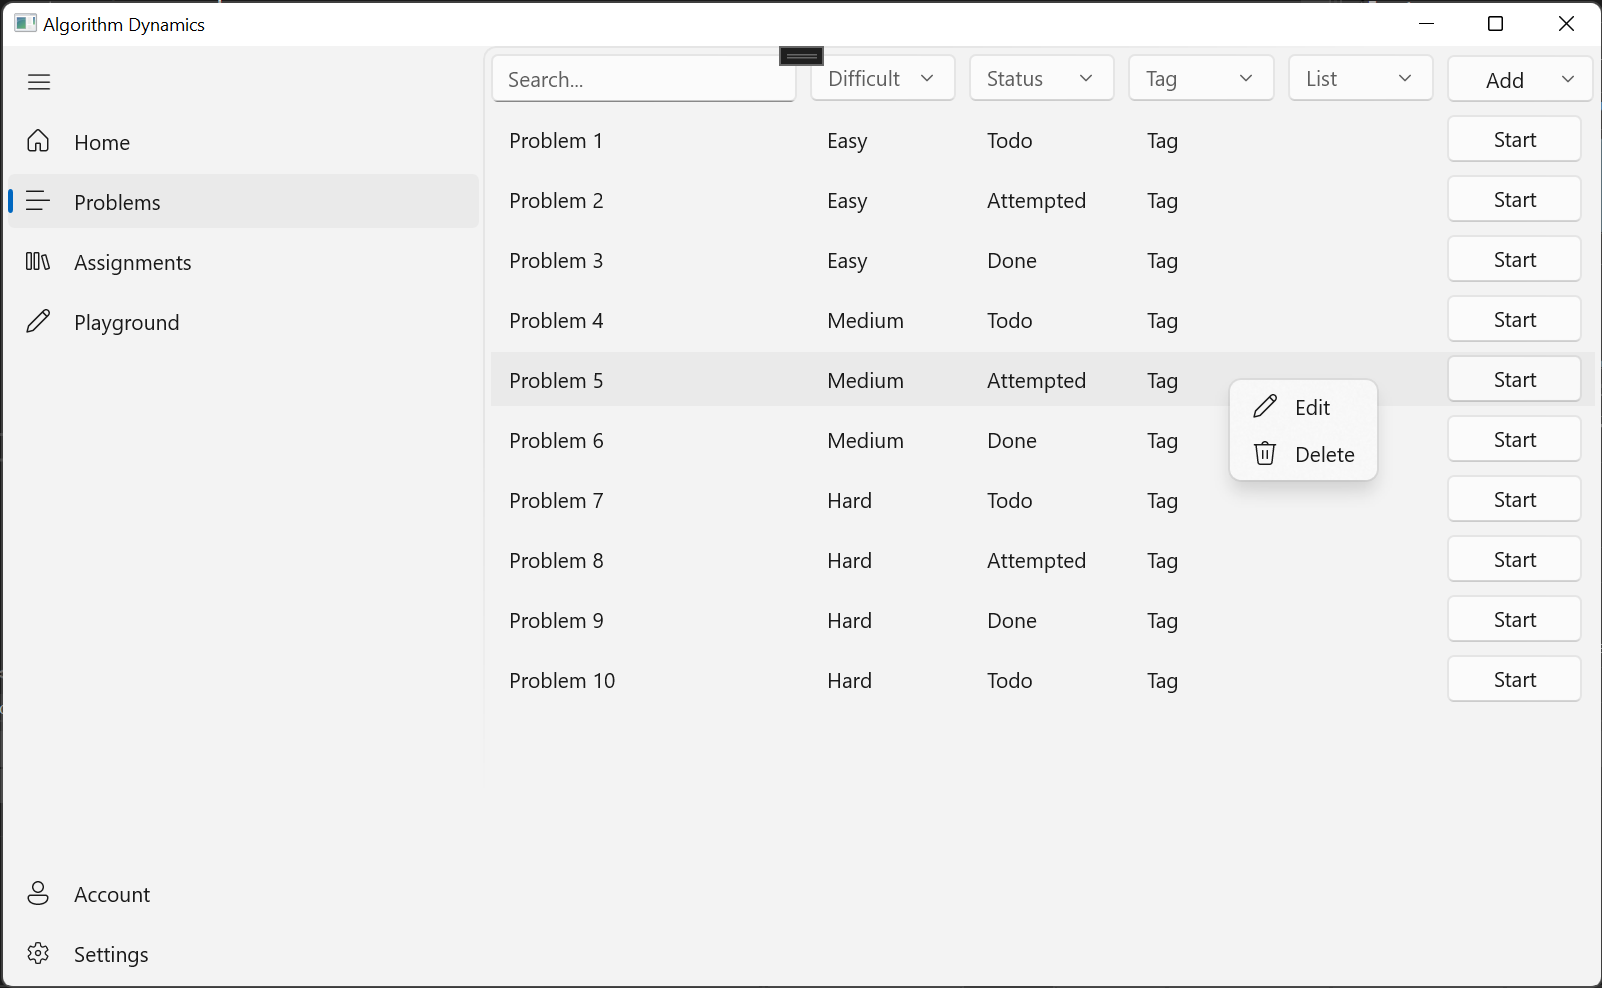
\includegraphics[width=\textwidth, height=\textheight, keepaspectratio]{ProblemsPage-SingleSelected-Flyout}

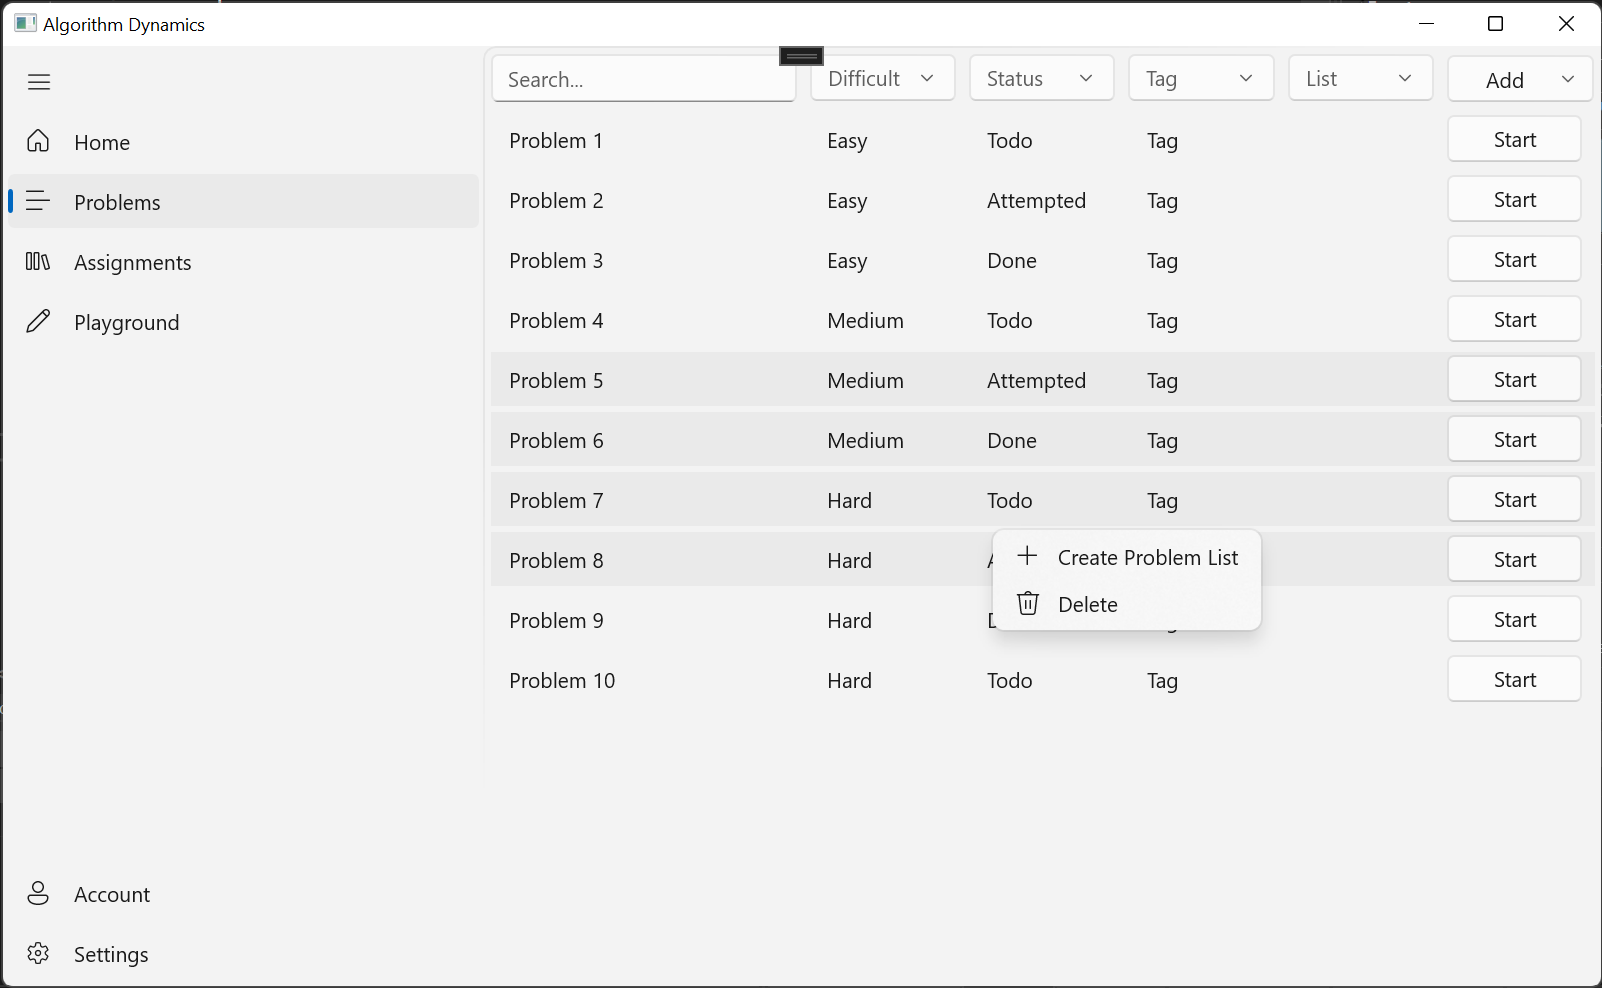
\includegraphics[width=\textwidth, height=\textheight, keepaspectratio]{ProblemsPage-MultipleSelected-Flyout}

Similarly, I can add the delete content dialog for these flyouts and leave the edit and create new problem list feature in the future.

\begin{minted}{csharp}
/// <summary>
/// Edit the selected Problem
/// Navigate to the EditProblemPage
/// </summary>
/// <param name="sender"></param>
/// <param name="e"></param>
private void EditProblem(object sender, RoutedEventArgs e)
{
    // TODO Navigate to the EditProblemPage
    throw new NotImplementedException();
}

/// <summary>
/// Show a content dialog to confirm the deletion of a Problem
/// </summary>
/// <param name="sender"></param>
/// <param name="e"></param>
/// <exception cref="NotImplementedException"></exception>
private async void DeleteProblem(object sender, RoutedEventArgs e)
{
    ContentDialog dialog = new ContentDialog();
    dialog.Title = "Delete Problem";
    dialog.PrimaryButtonText = "Delete";
    dialog.CloseButtonText = "Cancel";
    dialog.Content = $"Are you sure that you want to permanently delete {(ProblemsListView.SelectedItem as Problem).Name}?";
    dialog.DefaultButton = ContentDialogButton.Close;
    dialog.XamlRoot = this.Content.XamlRoot;
    var result = await dialog.ShowAsync();
    if (result == ContentDialogResult.Primary)
    {
        // TODO Delete the selected problem
        throw new NotImplementedException();
    }
}

/// <summary>
/// Create a new ProblemList from multiple selected items
/// Navigate to the CreateProblemListPage
/// </summary>
/// <param name="sender"></param>
/// <param name="e"></param>
/// <exception cref="NotImplementedException"></exception>
private void CreateProblemList(object sender, RoutedEventArgs e)
{
    // TODO Navigate to the CreateProblemList
    throw new NotImplementedException();
}

/// <summary>
/// Show a content dialog to confirm the deletion of Problems
/// </summary>
/// <param name="sender"></param>
/// <param name="e"></param>
/// <exception cref="NotImplementedException"></exception>
private async void DeleteProblems(object sender, RoutedEventArgs e)
{
    ContentDialog dialog = new ContentDialog();
    dialog.Title = "Delete Problem";
    dialog.PrimaryButtonText = "Delete";
    dialog.CloseButtonText = "Cancel";
    dialog.Content = $"Are you sure that you want to permanently delete these {ProblemsListView.SelectedItems.Count} Problems?";
    dialog.DefaultButton = ContentDialogButton.Close;
    dialog.XamlRoot = this.Content.XamlRoot;
    var result = await dialog.ShowAsync();
    if (result == ContentDialogResult.Primary)
    {
        // TODO Delete the selected problems
        throw new NotImplementedException();
    }
}
\end{minted}

Finally, for the ProblemsPage, I need to handle the searh query. The ProblemListView needs to be updated when different search queries are entered in the toolbar. I create a \code{Search} procedure to handle the searc event. When the user select an option in the ComboBoxes, or enter the search box, the \code{Search} procedure will be called. All data will be passed to a \code{Query} function that returns searching result. For now, because the database is not implemented, I will just return the query. The \code{Query} function will be implemented in the future.

\begin{minted}{csharp}
/// <summary>
/// Search the problem lists that under conditions
/// </summary>
/// <param name="sender"></param>
/// <param name="args"></param>
private void Search(object sender, object args)
{
    var keywords = ProblemsSearchBox.Text;
    var difficulty = DifficultyComboBox.SelectedValue?.ToString();
    var status = StatusComboBox.SelectedValue?.ToString();
    var tag = TagComboBox.SelectedValue?.ToString();
    var list = ListComboBox.SelectedValue?.ToString();
    // TODO Query(keywords, difficulty, status, tag, list);
    Problems.Clear();
    Problems.Add(new Problem(keywords, difficulty, status, tag));
}
\end{minted}

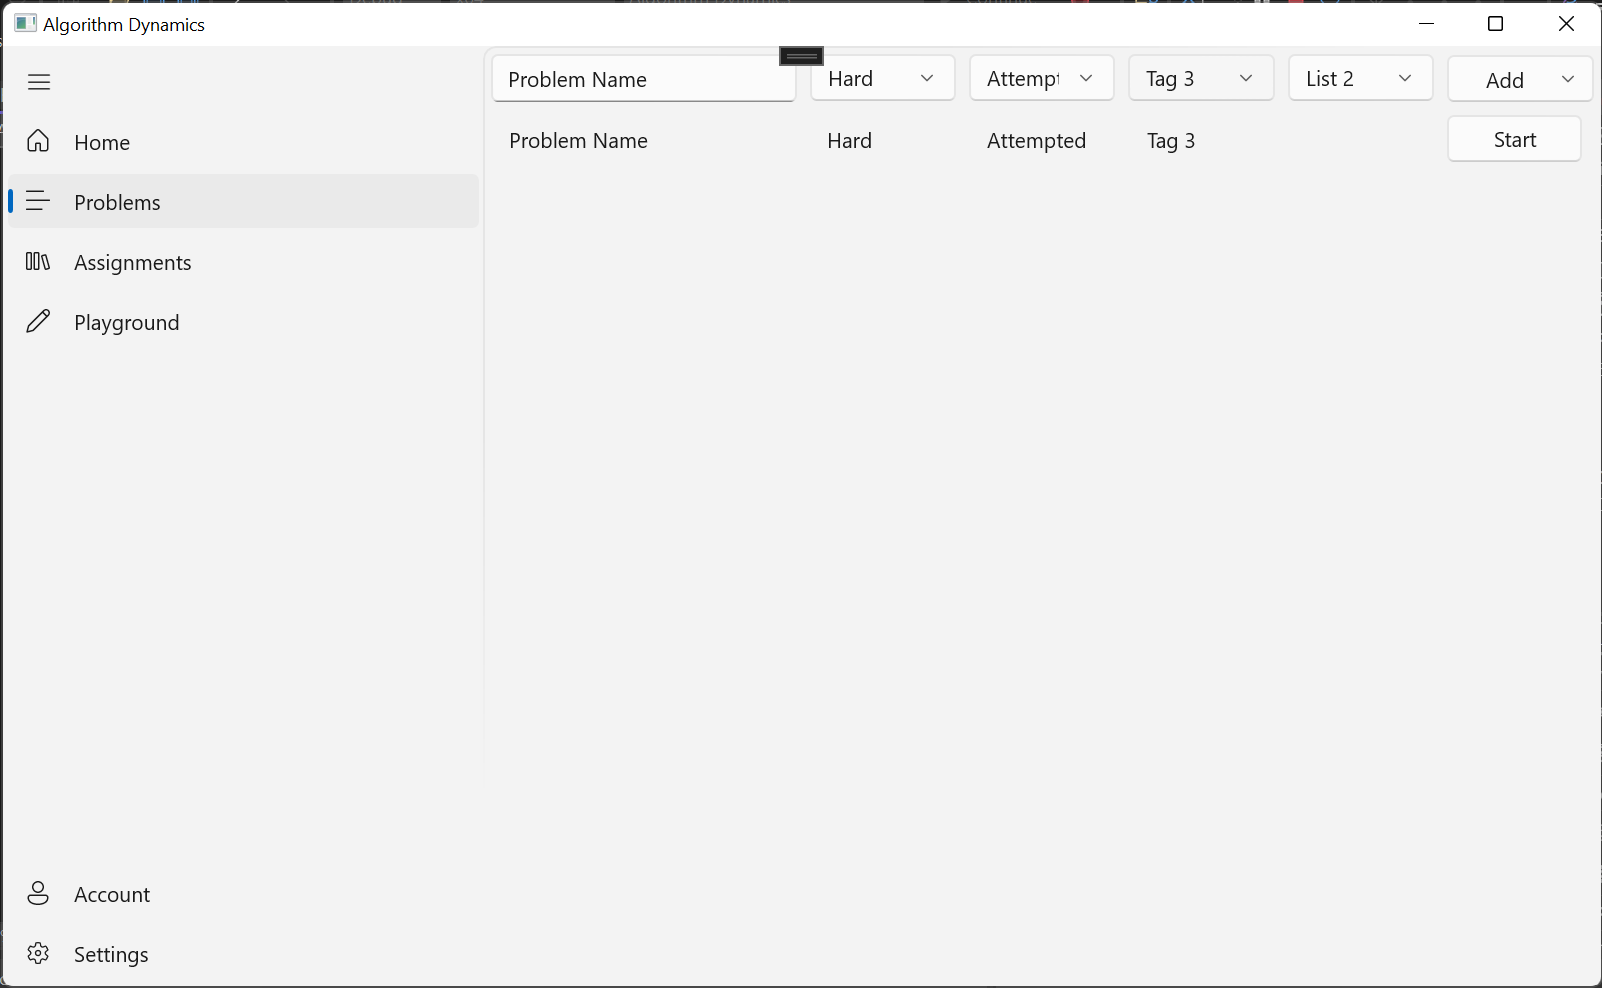
\includegraphics[width=\textwidth, height=\textheight, keepaspectratio]{ProblemsPage-Search}

The correct search result is returned and the search result is updated correctly when different search conditions are selected.

\subsubsection{Testing and validation}

\begin{tabulary}{\linewidth}{|L|l|L|}
    \hline
    Test & Result & Remark \\
    \hline
    Does it load & Pass & \\
    \hline
    Does the toolbar display correctly & Pass & \\
    \hline
    Does the toolbar interact correctly & Pass & \\
    \hline
    Does the toolbar return the correct search result & Failed & The search algorithm will be implemented after the database and data structure is ready in the future milestones. \\
    \hline
    Does the add button work & Failed & The data import and create new problem function will be implemented after the CreateNewProblemPage and the data import function is implemented. \\
    \hline
    Does the problem list show up correct & Pass & \\
    \hline
    Does the start button work & Failed & The start button will be implemented after the coding page is implemented. \\
    \hline
    Does the selection and menu flyout work & Failed & The delete and edit button will be implemented after the database is ready. \\
    \hline
\end{tabulary}

The ProblemsPage is partially implemented with many todos left for the future. But in this iteration, it is good to go as all UI elements are ready. I will move on to the PlaygroundPage and CodingPage next.

\subsection{Create the PlaygroundPage}

\subsubsection{Implementation}

The main component in the PlaygroundPage is the Code Editor. Because the CodingPage will need to use the Code Editor as well, so I will set the Code Editor as a custom control so it can be reused later.

The Code Editor needs to support line number, syntax highlighting, and other editing features. It is too complex for this project to implement all of these by hand. So I will use a third-party library to achieve that. I am using the \href{https://microsoft.github.io/monaco-editor/}{Monaco Editor} for this purpose.

I create a custom control for the editor so I can reuse it later in different pages easily.

\begin{minted}{xml}
<UserControl
    x:Class="Algorithm_Dynamics.Controls.CodeEditor"
    xmlns="http://schemas.microsoft.com/winfx/2006/xaml/presentation"
    xmlns:x="http://schemas.microsoft.com/winfx/2006/xaml"
    xmlns:local="using:Algorithm_Dynamics.Controls"
    xmlns:d="http://schemas.microsoft.com/expression/blend/2008"
    xmlns:mc="http://schemas.openxmlformats.org/markup-compatibility/2006"
    mc:Ignorable="d">

    <TextBlock Text="CodeEditor"/>
</UserControl>
\end{minted}

\begin{minted}{csharp}
using Microsoft.UI.Xaml.Controls;

namespace Algorithm_Dynamics.Controls
{
    public sealed partial class CodeEditor : UserControl
    {
        public CodeEditor()
        {
            InitializeComponent();
        }
    }
}
\end{minted}

I import the control in the PlaygroundPage to verify its working.

\begin{minted}{xml}
<Page
    x:Class="Algorithm_Dynamics.Pages.PlaygroundPage"
    xmlns="http://schemas.microsoft.com/winfx/2006/xaml/presentation"
    xmlns:x="http://schemas.microsoft.com/winfx/2006/xaml"
    xmlns:local="using:Algorithm_Dynamics.Pages"
    xmlns:controls="using:Algorithm_Dynamics.Controls"
    xmlns:d="http://schemas.microsoft.com/expression/blend/2008"
    xmlns:mc="http://schemas.openxmlformats.org/markup-compatibility/2006"
    mc:Ignorable="d"
    Background="{ThemeResource ApplicationPageBackgroundThemeBrush}">

    <Grid>
        <controls:CodeEditor/>
    </Grid>
</Page>
\end{minted}

Now, when I run the application and navigate to the PlaygroundPage I can see the Code Editor is displayed correctly.

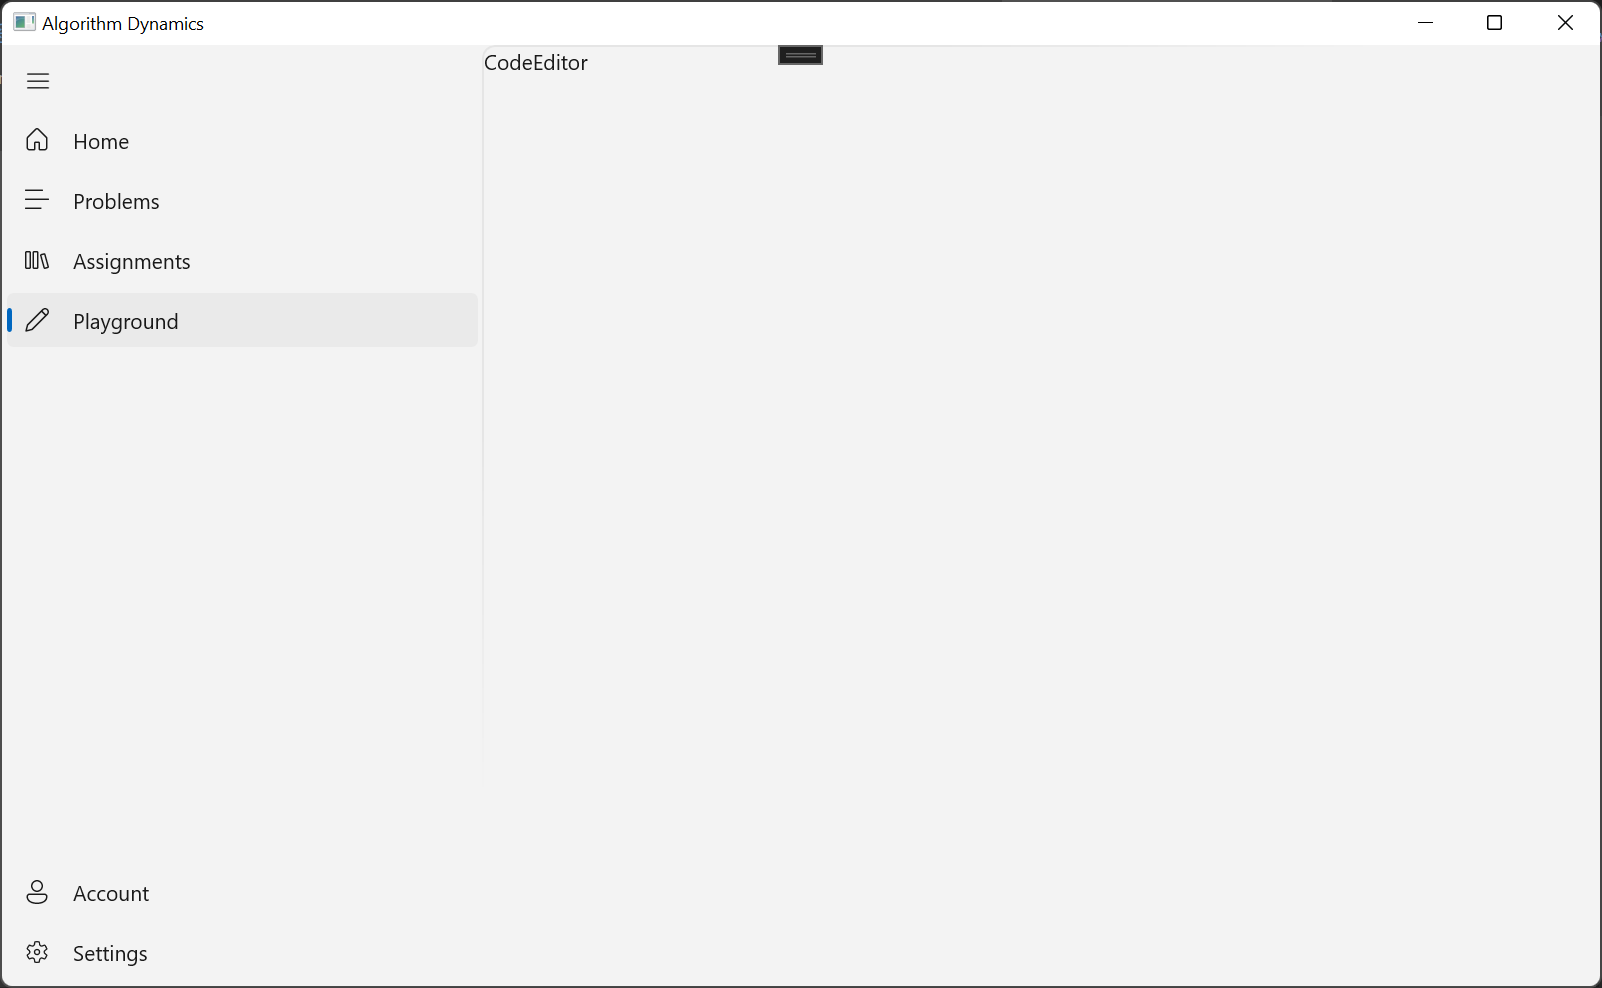
\includegraphics[width=\textwidth, height=\textheight, keepaspectratio]{CodeEditorControl}

The Monaco Editor is a web application, which means it needs to run in a browser. To use it, I need to use WebView2 component to load a HTML file, and initialize the Monaco Editor inside that webpage. The WebView2 control launches a Chromium instance and allows me to integrate webpages inside my app. I use the WebView2 control to load the HTML file. Before I create the webpage for the Monaco Editor, I place the WebView2 control and test it out.

\begin{minted}{xml}
<WebView2 
    x:Name="WebView"
    HorizontalAlignment="Stretch"
    VerticalAlignment="Stretch"
    Source="https://ocr.org.uk"/>
\end{minted}

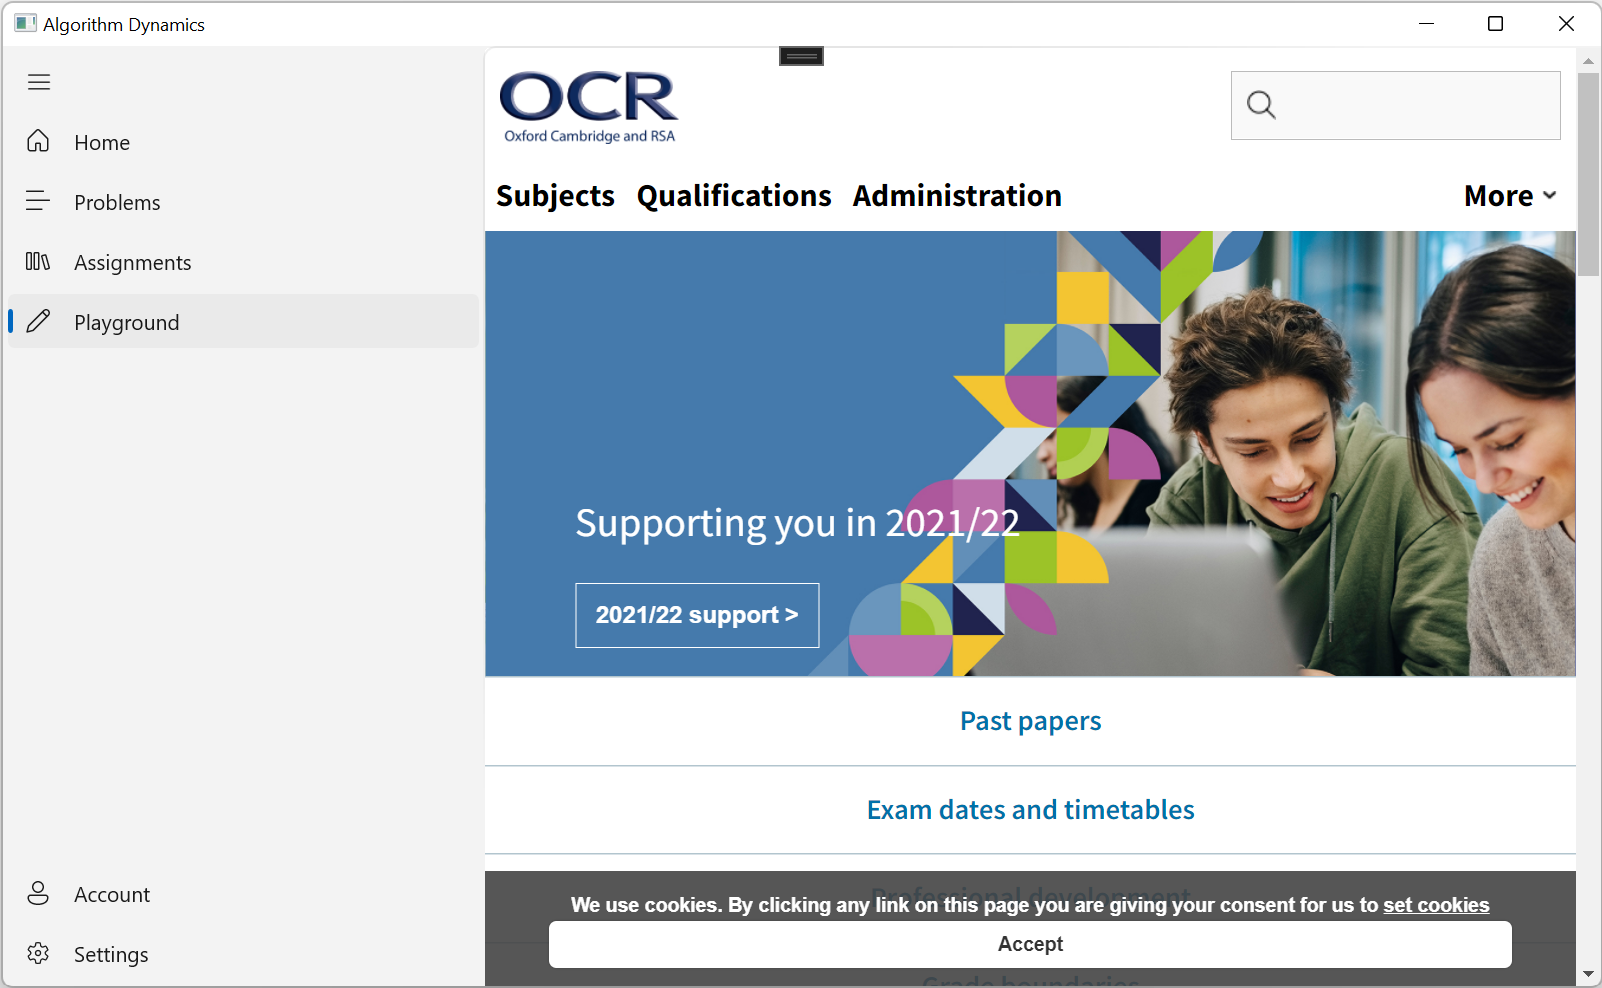
\includegraphics[width=\textwidth, height=\textheight, keepaspectratio]{PlaygroundPage-WebView2-Webpage}

I set the source of the WebView2 control to the offcial website of OCR, and it loads up correctly. Now I can start working on the webpage for the editor. To load a local HTML file, I need to set a mapping relationship between a URL space and a local folder.

\begin{minted}{csharp}
/// <summary>
/// Initialize the WebView control and load Editor.html
/// </summary>
async void InitializeWebViewAsync()
{
    // Ensure the CoreWebView2 is loaded
    await WebView.EnsureCoreWebView2Async();

    // Set the mapping
    StorageFolder AssetsDirectory = await Package.Current.InstalledLocation.GetFolderAsync(@"Assets");
    WebView.CoreWebView2.SetVirtualHostNameToFolderMapping(
        "localeditor.algorithmdynamics.com",
        AssetsDirectory.Path,
        CoreWebView2HostResourceAccessKind.Allow
    );

    // Load Editor.html
    WebView.Source = new Uri("http://localeditor.algorithmdynamics.com/Editor.html");
}
\end{minted}

Now I can load Editor.html under the Assets folder. I use a sample HTML file to test it out.

\begin{minted}{html}
<!DOCTYPE html>
<html lang="en">
<head>
    <meta charset="UTF-8">
    <meta http-equiv="X-UA-Compatible" content="IE=edge">
    <meta name="viewport" content="width=device-width, initial-scale=1.0">
    <title>Document</title>
</head>
<body>
    <h1>Hello Editor!</h1>
</body>
</html>
\end{minted}

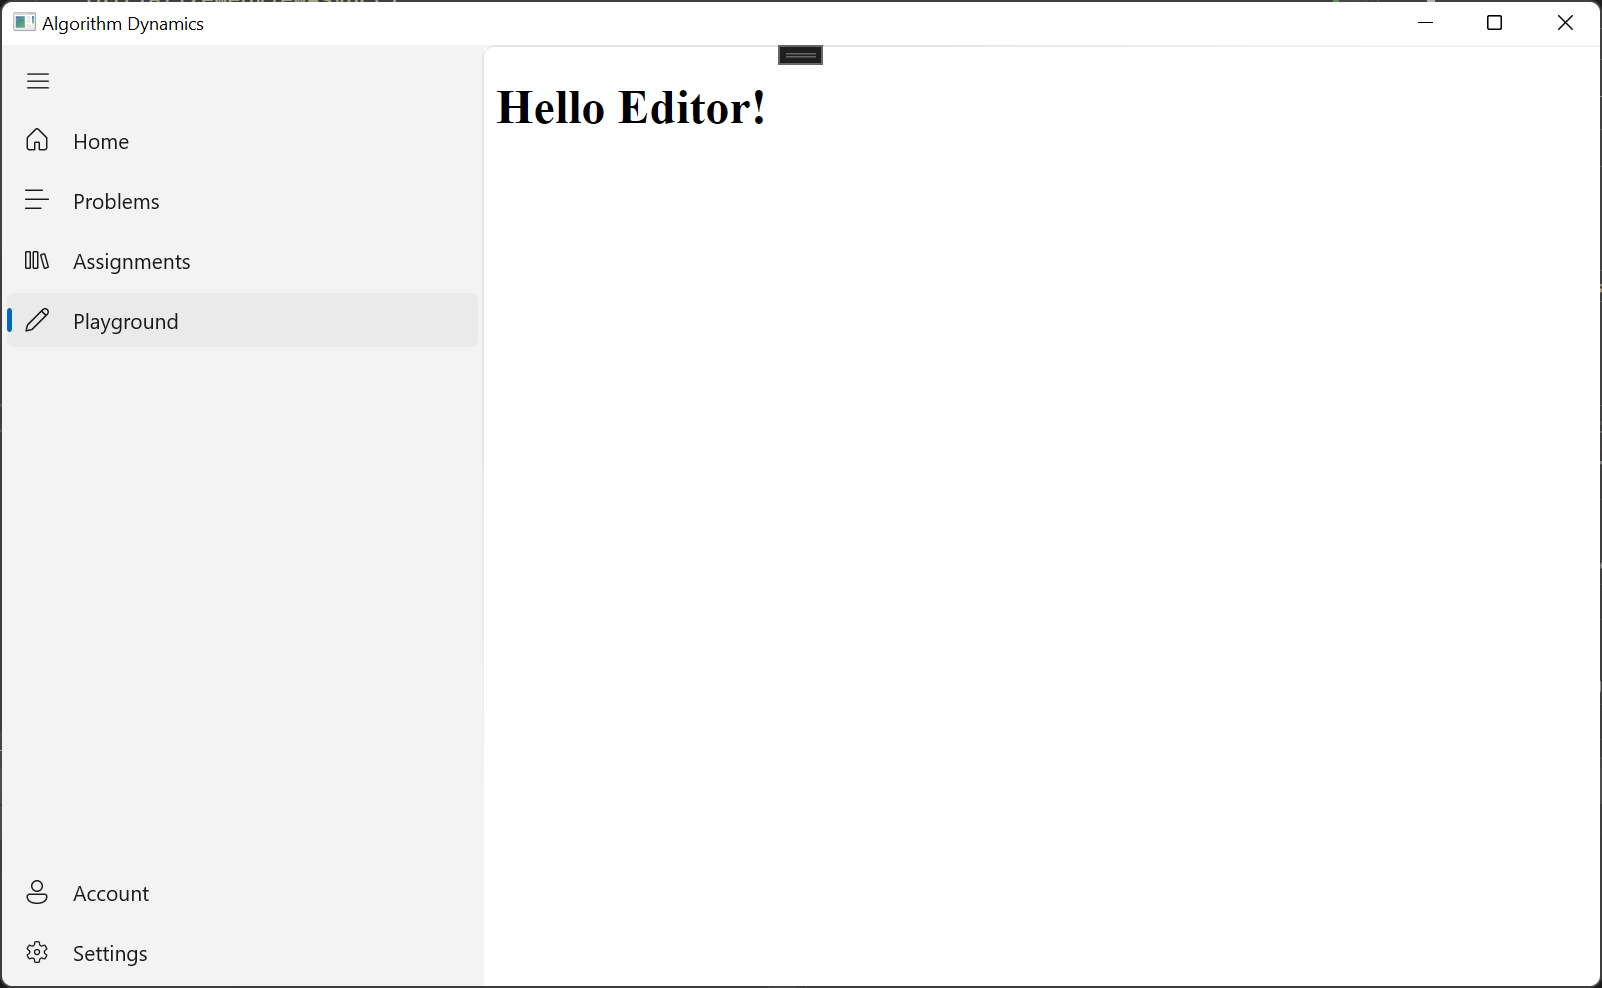
\includegraphics[width=\textwidth, height=\textheight, keepaspectratio]{PlaygroundPage-WebView2-HelloEditor}

The h1 title ``Hello Editor!'' is displayed correctly, which means the local file is loaded as expected. Now I can import the Monaco Editor to the WebView2 control.

\begin{minted}{html}
<body>
    <div id="container" style="width:800px;height:600px;border:1px solid grey"></div>

    <script src="monaco-editor/min/vs/loader.js"></script>
    <script>
        require.config({ paths: { vs: 'monaco-editor/min/vs' } });
        require(['vs/editor/editor.main'], () => {
            window.editor = monaco.editor.create(document.getElementById('container'), {
                value: ['function x() {', '\tconsole.log("Hello Editor!");', '}'].join('\n'),
                language: 'javascript'
            });
        });
    </script>
</body>
\end{minted}

I add a container in the body to host the instance of the editor. Then I write some JavaScript code to import the editor and initialize it with a sample code.

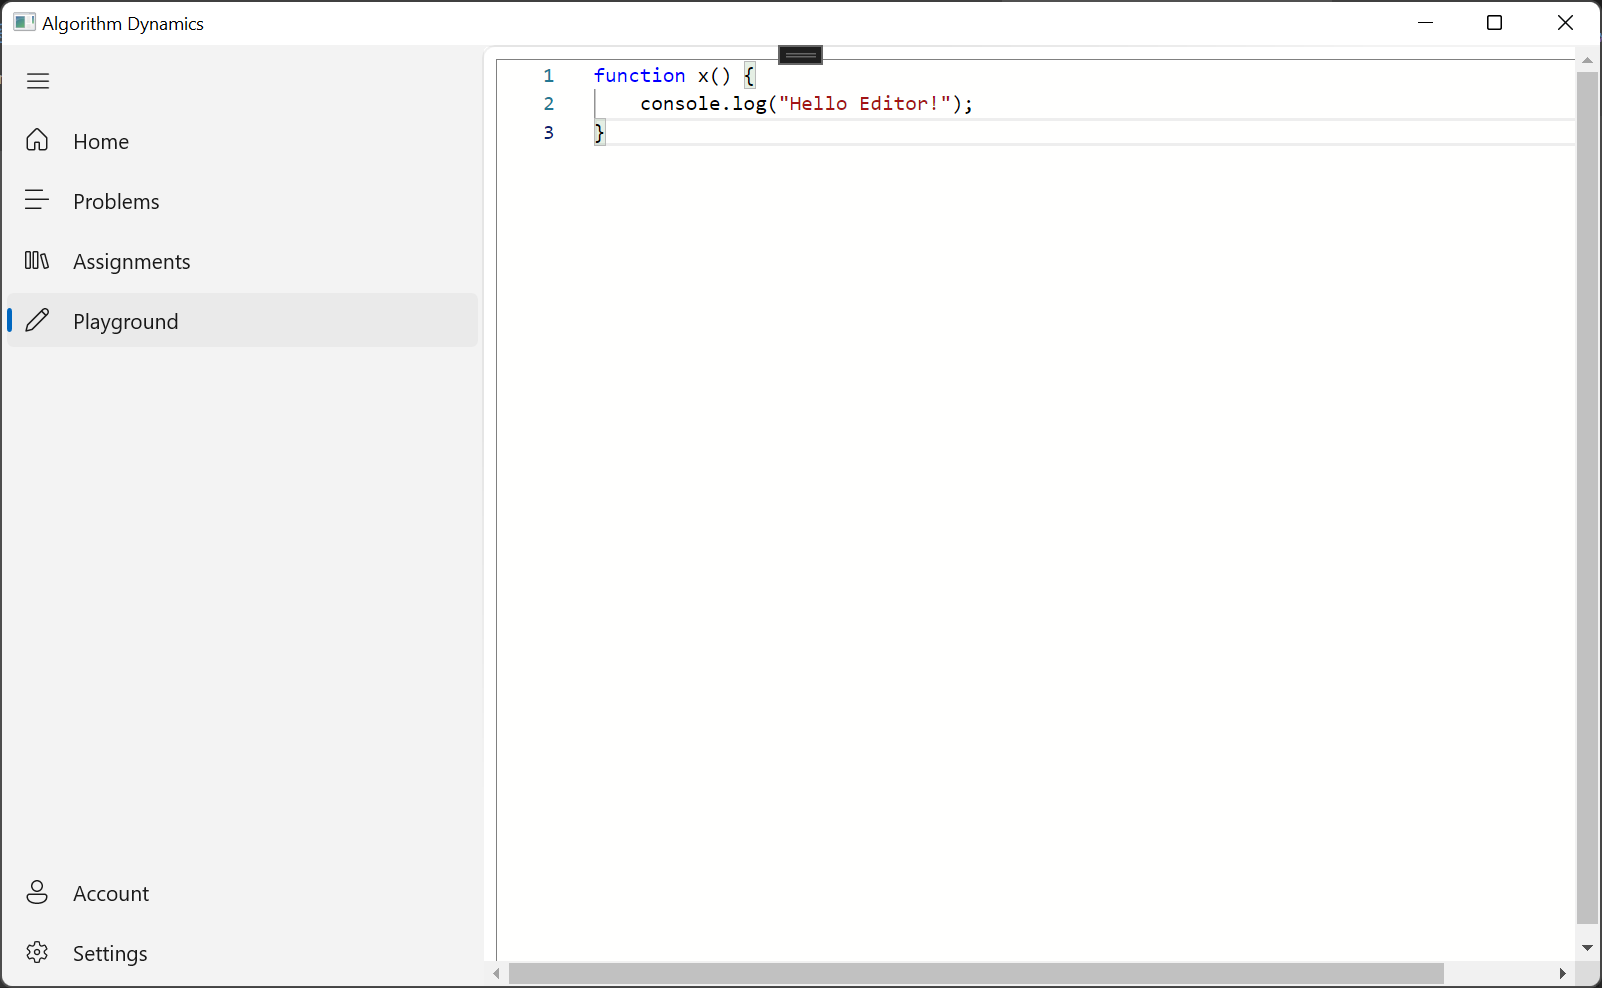
\includegraphics[width=\textwidth, height=\textheight, keepaspectratio]{PlaygroundPage-WebView2-EditorLoaded}

The editor is now loaded correctly with the sample code. I can type in the editor and utlize all powerful functions of the Monaco Editor.

But I find that the editor has a fixed height and width. On a small screen like the screen shot, you can see the scroll bars. And on a larger display, the editor will not occupy the entire screen. I need to adjust its style to make it responsive.

I add some CSS code to set the height and width of the editor to 100\%.

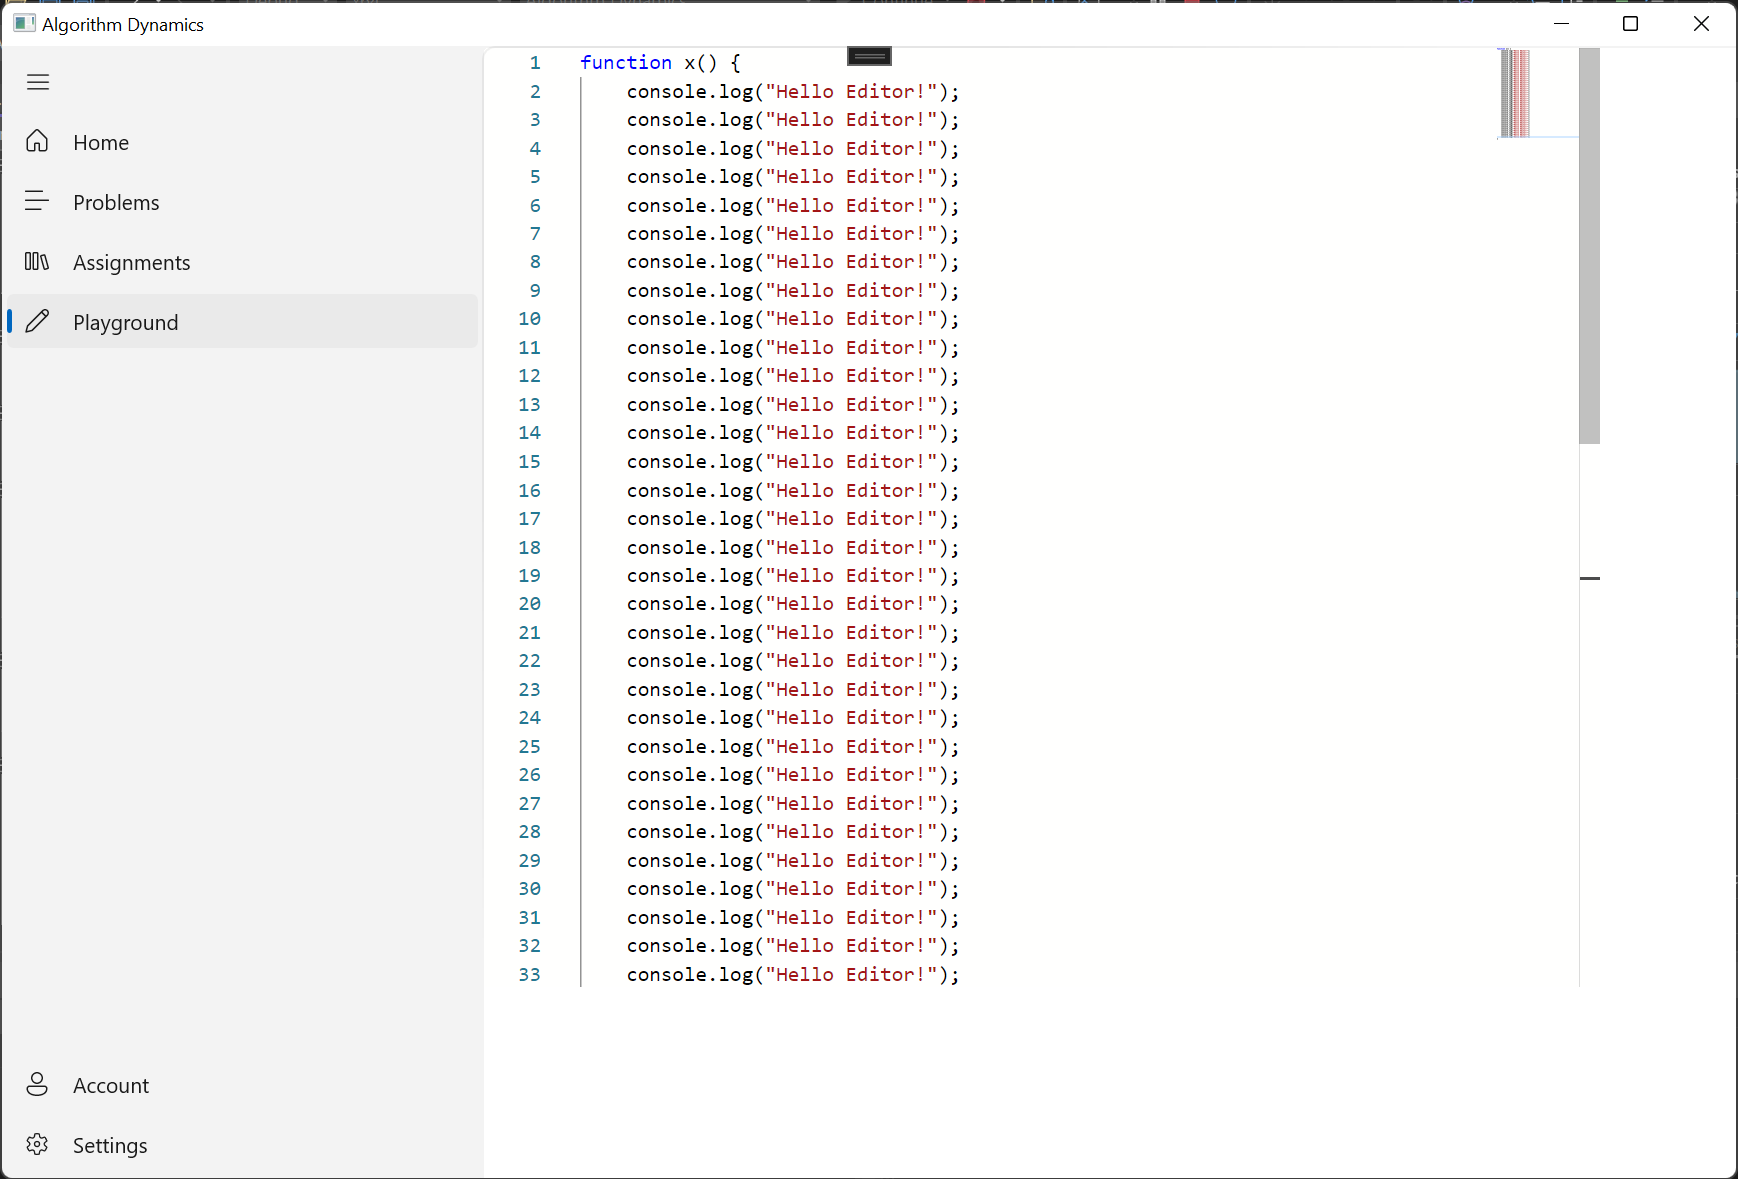
\includegraphics[width=\textwidth, height=\textheight, keepaspectratio]{PlaygroundPage-WebView2-ResizeFailed}

Now, the scroll bars are gone. But when I resize the window, the editor still does not follow the window size. After reading the documentation of the Monaco Editor, I find out that I need to manually call the \code{editor.layout()} function to recalculate the editor size.

\begin{minted}{html}
<script>
    window.addEventListener("resize", () => editor.layout());
</script>
\end{minted}

By adding the event handler for the window resize event and call the layout function, the editor can now resize correctly according to the window size.

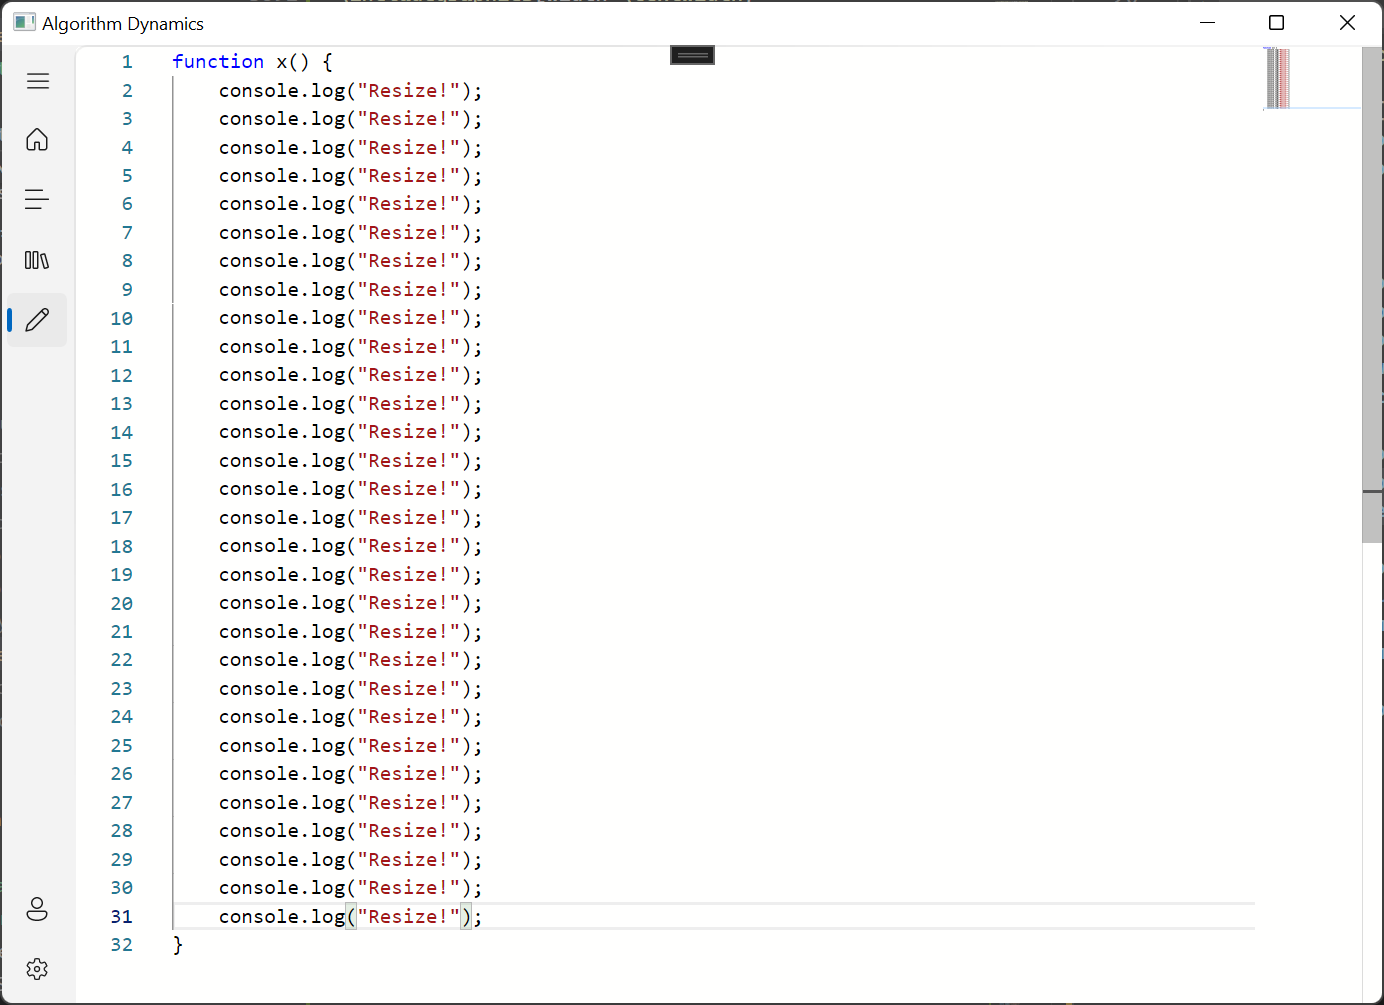
\includegraphics[width=\textwidth, height=\textheight, keepaspectratio]{PlaygroundPage-WebView2-ResizeSuccess}

Before I go any further, I need to first implement the PlaygroundPage, so I have a working environment to test the editor out.

\begin{minted}{xml}
<Page
    x:Class="Algorithm_Dynamics.Pages.PlaygroundPage"
    xmlns="http://schemas.microsoft.com/winfx/2006/xaml/presentation"
    xmlns:x="http://schemas.microsoft.com/winfx/2006/xaml"
    xmlns:local="using:Algorithm_Dynamics.Controls"
    xmlns:controls="using:CommunityToolkit.WinUI.UI.Controls"

    xmlns:d="http://schemas.microsoft.com/expression/blend/2008"
    xmlns:mc="http://schemas.openxmlformats.org/markup-compatibility/2006"
    mc:Ignorable="d"
    Background="{ThemeResource ApplicationPageBackgroundThemeBrush}">

    <Grid>
        <Grid.RowDefinitions>
            <RowDefinition Height="*"/>
            <RowDefinition Height="*"/>
            <RowDefinition Height="auto"/>
        </Grid.RowDefinitions>

        <Grid.ColumnDefinitions>
            <ColumnDefinition Width="*"/>
            <ColumnDefinition Width="*"/>
        </Grid.ColumnDefinitions>

        <!-- ... -->
    </Grid> 
</Page>
\end{minted}

I will use a grid with 3 rows and 2 columns to hold all controls.

\begin{minted}{xml}
<local:CodeEditor
    x:Name="CodeEditor"
    Grid.Row="0"
    Grid.Column="0"
    Grid.RowSpan="2"
    Margin="0 0 8 0"/>

<TextBox
    x:Name="OutputBox"
    Grid.Row="0"
    Grid.Column="1"
    Margin="8 0 0 8"
    PlaceholderText="Output"
    IsSpellCheckEnabled="False"
    AcceptsReturn="True"/>

<TextBox
    x:Name="InputBox"
    Grid.Row="1"
    Grid.Column="1"
    Margin="8 8 0 0"
    PlaceholderText="Input"
    IsSpellCheckEnabled="False"
    AcceptsReturn="True"/>

<Grid
    Grid.Row="2"
    Grid.Column="0">
    <ComboBox
        x:Name="LanguageComboBox"
        SelectedIndex="0"
        VerticalAlignment="Stretch">
        <x:String>Python</x:String>
        <x:String>C</x:String>
        <x:String>C++</x:String>
    </ComboBox>
</Grid>

<Grid
    Grid.Row="2"
    Grid.Column="1"
    Margin="8 0 0 0">
    <Grid.RowDefinitions>
        <RowDefinition Height="auto"/>
        <RowDefinition Height="*"/>
    </Grid.RowDefinitions>
    <Grid.ColumnDefinitions>
        <ColumnDefinition Width="*"/>
        <ColumnDefinition Width="*"/>
    </Grid.ColumnDefinitions>
    <ProgressBar
        Grid.Row="0"
        Grid.Column="0"
        Grid.ColumnSpan="2"
        HorizontalAlignment="Stretch"
        VerticalAlignment="Stretch"
        IsIndeterminate="True"
        ShowPaused="False"
        ShowError="False" />
    <TextBlock
        x:Name="StatusTextBlock"
        Grid.Row="1"
        Grid.Column="0"
        HorizontalAlignment="Left"
        VerticalAlignment="Center"
        Text="Pending"/>
    <Button
        x:Name="RunCodeButton"
        Grid.Row="1"
        Grid.Column="1"
        HorizontalAlignment="Right"
        VerticalAlignment="Stretch"
        Content="Run Code"
        Click="RunCodeButton_Click"/>
</Grid>
\end{minted}

To allow different sections to be resizeable, I add two grid splitters to the grid.

\begin{minted}{xml}
<controls:GridSplitter
    HorizontalAlignment="Left"
    Grid.Column="1"
    Grid.RowSpan="2"
    Width="16">
    <controls:GridSplitter.RenderTransform>
        <TranslateTransform X="-8" />
    </controls:GridSplitter.RenderTransform>
</controls:GridSplitter>

<controls:GridSplitter
    VerticalAlignment="Top"
    Grid.Row="1"
    Grid.Column="1"
    Grid.ColumnSpan="1"
    Margin="8 0 0 0"
    Height="16">
    <controls:GridSplitter.RenderTransform>
        <TranslateTransform Y="-8"/>
    </controls:GridSplitter.RenderTransform>
</controls:GridSplitter>
\end{minted}

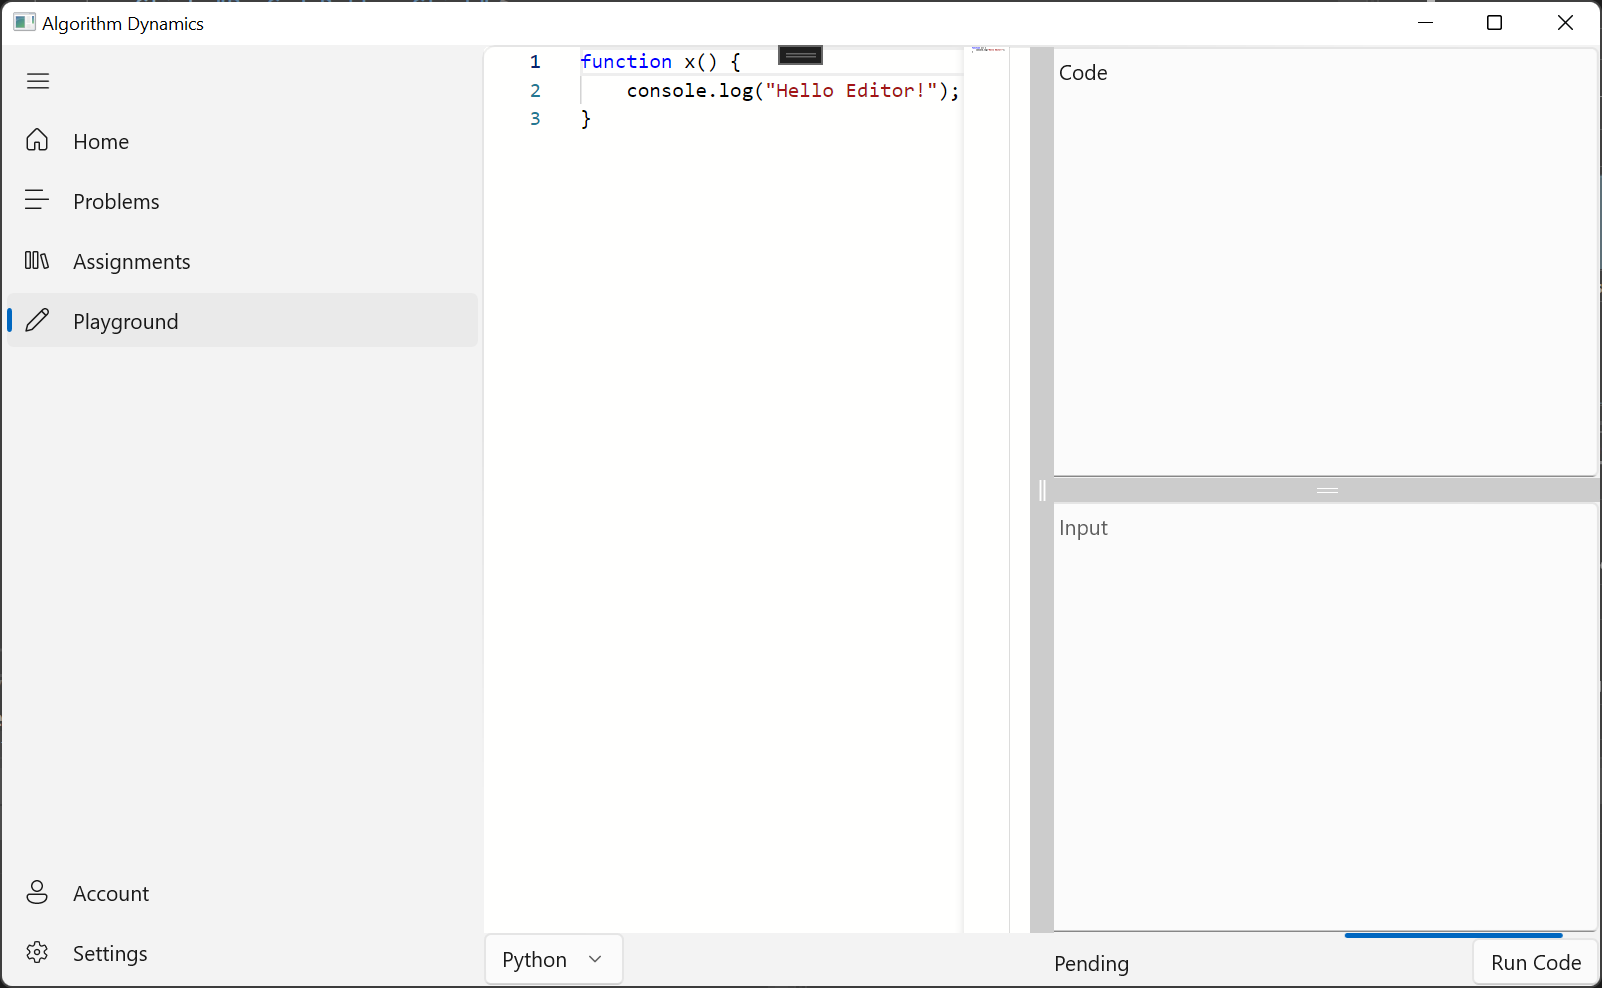
\includegraphics[width=\textwidth, height=\textheight, keepaspectratio]{PlaygroundPage-Layout}

All controls work correctly and they can be resized by the grid splitter. Now I need to interact with the code editer. I need to be able to get the code inside, set its programming language and color theme. To pass the config data to the editor, I will need to serialize the data into a JSON string and send it through web message. To avoid hand crafting the JSON string, I create a new class \code{EditorConfig} and use the \code{System.Text.Json} library to serialize the data.

\begin{minted}{csharp}
public class EditorConfig
{
    public EditorConfig(string theme, string language, string code)
    {
        Theme = theme;
        Language = language;
        Code = code;
    }
    public string? Theme { get; set; } = null;
    public string? Language { get; set; } = null;
    public string? Code { get; set; } = null;
}
\end{minted}

I then create a helper function to send the config data to the editor. It takes in an instance of the EditorConfig and serializes it into a JSON string, then send it through a web message. And for the testing purpose, I send the message when initializing the editor.

\begin{minted}{csharp}
/// <summary>
/// Update the editor config of the Monaco Editor
/// </summary>
/// <param name="editorConfig"></param>
private void UpdateEditorConfig(EditorConfig editorConfig)
{
    WebView.CoreWebView2.PostWebMessageAsJson(JsonSerializer.Serialize(editorConfig));
}


async void InitializeWebViewAsync()
{
    // ...
    UpdateEditorConfig(new EditorConfig("vs-dark", "python", "print(1)"));
}
\end{minted}

On the web end, I need to listen to the web message and process the data received.

\begin{minted}{javascript}
// Receive and set theme/language/code
window.chrome.webview.addEventListener('message', (e) => {
    console.log(e)
    let data = e.data
    if (data.Theme) monaco.editor.setTheme(data.Theme)
    if (data.Language) monaco.editor.setModelLanguage(window.editor.getModel(), data.Language)
    if (data.Code) window.editor.getModel().setValue(data.Code)
})
\end{minted}

Now, when I open the PlaygroundPage, a code editor with dark theme and syntax highlighting for Python should be loaded.

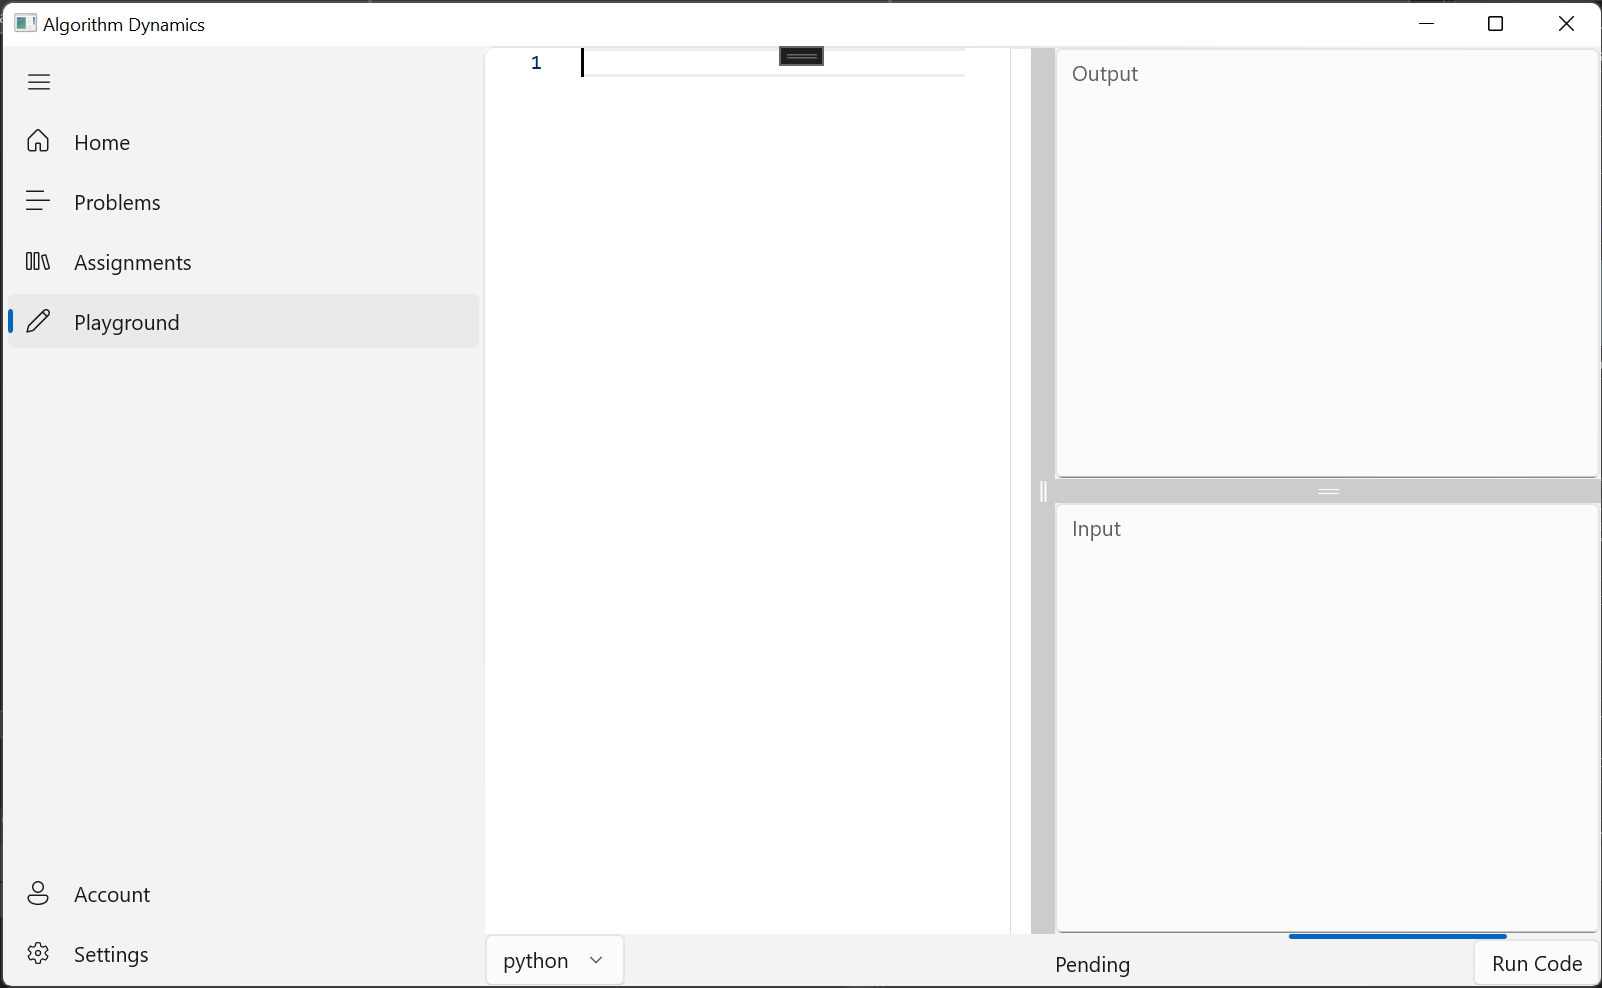
\includegraphics[width=\textwidth, height=\textheight, keepaspectratio]{PlaygroundPage-EditorConfig-NotLoading}

However, it is clearly not loading. Neither the theme, the syntax highlighting nor the code is set. It is clear that the config has not been passed correctly. When I open the devtool, nothing is in the output, which means that \code{console.log(e)} has not been called.

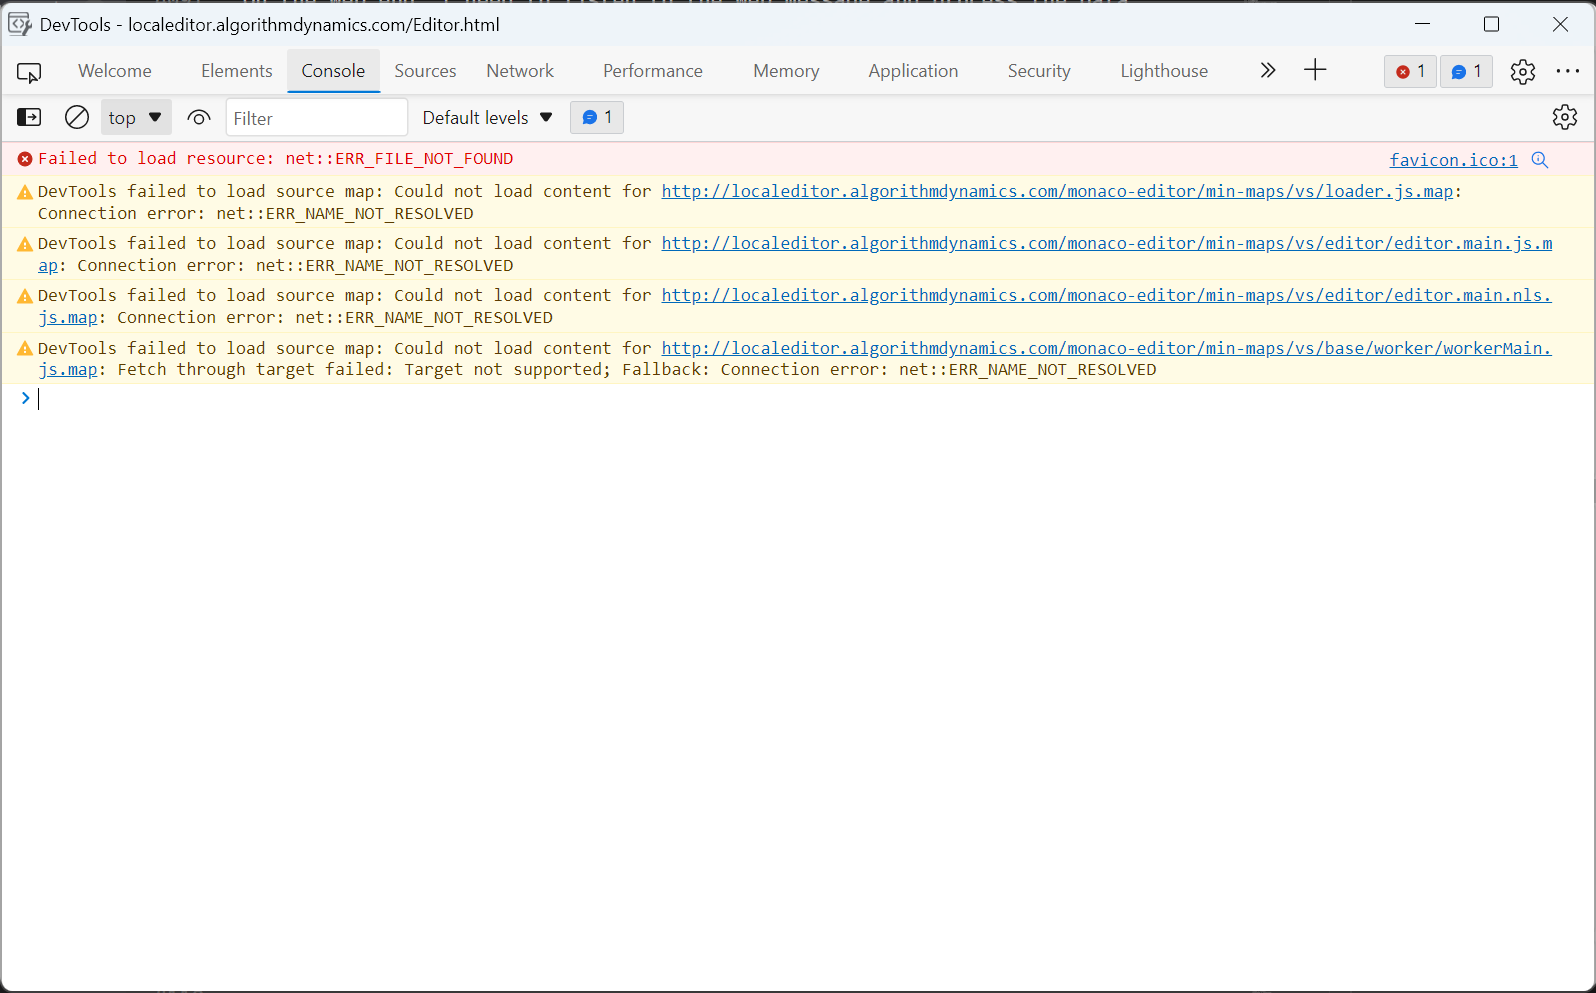
\includegraphics[width=\textwidth, height=\textheight, keepaspectratio]{PlaygroundPage-EditorConfig-NotLoading-Devtool}

I suspect this is caused by the fact that at the time the web message is sent, the Monaco Editor is not fully loaded, therefore it has not started listening for the message. To test my hypothesis, instead of sending a message, I will inject a JavaScript script to pass the value through the global window object.

\begin{minted}{csharp}
async void InitializeWebViewAsync()
{
    // ...
    var editorConfig = new EditorConfig("vs-dark", "python", "print(1)");
    await WebView.ExecuteScriptAsync($"window.config={JsonSerializer.Serialize(editorConfig)}");
}
\end{minted}

And on the web end, I initialize the editor with the config data.

\begin{minted}{javascript}
window.editor = monaco.editor.create(document.getElementById('container'), {
    value: window.config?.Code,
    language: window.config?.Language,
    theme: window.config?.Theme
})
\end{minted}

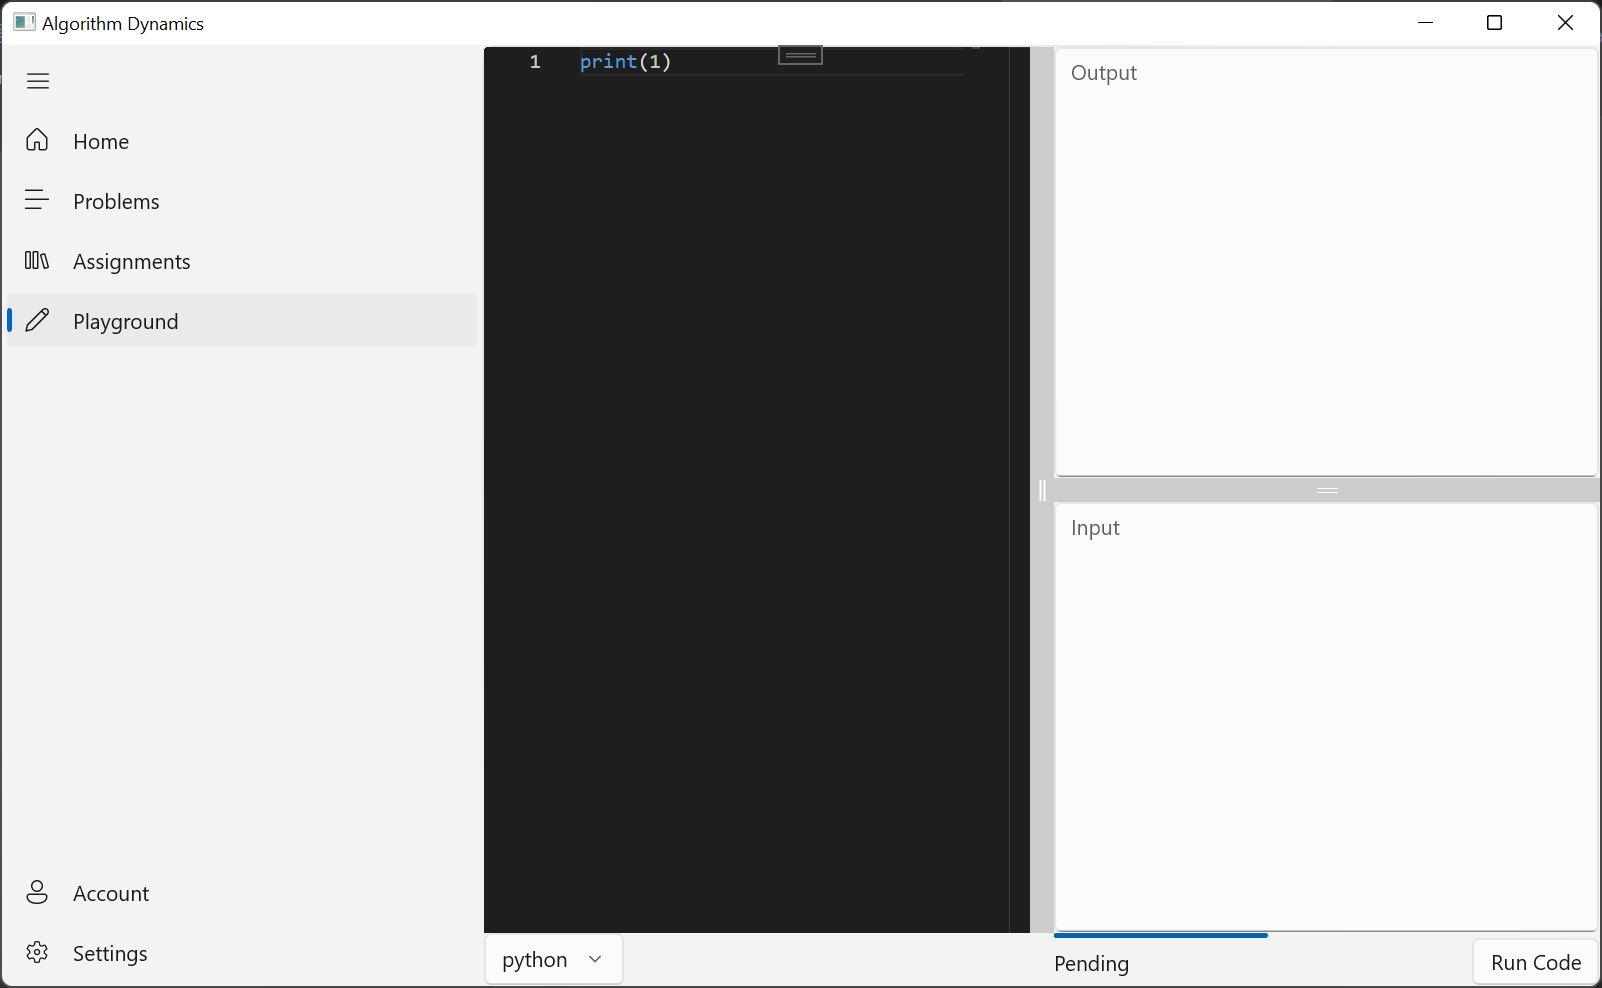
\includegraphics[width=\textwidth, height=\textheight, keepaspectratio]{PlaygroundPage-EditorConfig-Loading}

Now the theme, code, and language config is passed correctly, which also proves my hypothesis is correct. This problem should only occur at the initializing stage. Once the editor is loaded, passing config through web message should work fine.

In order to allow other pages to set the config, I need to expose these three fields by registering them as properties.

\begin{minted}{csharp}
/// <summary>
/// Return the editor theme based on current requested theme
/// </summary>
/// <param name="theme"></param>
/// <returns></returns>
private static string GetTheme(ElementTheme theme)
{
    if (theme == ElementTheme.Dark) return "vs-dark";
    else if (theme == ElementTheme.Light) return "vs";
    return "vs";
}
public string Code
{
    get { return (string)GetValue(CodeProperty); }
    set { SetValue(CodeProperty, value); }
}

public static readonly DependencyProperty CodeProperty =
    DependencyProperty.Register(
        "Code",
        typeof(string),
        typeof(CodeEditor),
        new PropertyMetadata("")
    );

public string Lang
{
    get { return (string)GetValue(LangProperty); }
    set 
    {
        UpdateEditorConfig(new EditorConfig(null, value, null));
        SetValue(LangProperty, value);
    }
}

public static readonly DependencyProperty LangProperty =
    DependencyProperty.Register(
        "Lang",
        typeof(string),
        typeof(CodeEditor),
        new PropertyMetadata("")
    );

public new ElementTheme RequestedTheme
{
    get { return base.RequestedTheme; }
    set
    {
        UpdateEditorConfig(new EditorConfig(GetTheme(value), null, null));
        base.RequestedTheme = value;
    }
}
\end{minted}

Note that \code{UpdateEditorConfig} is called when the language or the requested theme is changed to update the settings. To convert the theme code used in my app into the format of the Monaco Editor, I create a custom helper \code{GetTheme} to do the conversion. And I update the initializing process to use the value from these variables.

\begin{minted}{csharp}
async void InitializeWebViewAsync()
{
    // ...
    var editorConfig = new EditorConfig(GetTheme(RequestedTheme), Lang, Code);
    await WebView.ExecuteScriptAsync($"window.config={JsonSerializer.Serialize(editorConfig)}");
}
\end{minted}

Now, in the PlaygroundPage, I can use the CodeEditor in this way.

\begin{minted}{xml}
<local:CodeEditor
    x:Name="CodeEditor"
    Grid.Row="0"
    Grid.Column="0"
    Grid.RowSpan="2"
    Margin="0 0 8 0"
    Code="hello world!"
    Lang="cpp"
    RequestedTheme="Dark"/>
\end{minted}

Now when I run the app, it should work just like before, but this time with its config exposed and set by the PlaygroundPage. However, I encounter the following exception.

\begin{minted}{text}
System.NullReferenceException
  HResult=0x80004003
  Message=Object reference not set to an instance of an object.
  Source=Algorithm Dynamics
  StackTrace:
   at Algorithm_Dynamics.Controls.CodeEditor.UpdateEditorConfig(EditorConfig editorConfig) in C:\Algorithm-Dynamics\src\Algorithm Dynamics\Controls\CodeEditor.xaml.cs:line 74
\end{minted}

The exception is caused by the \code{UpdateEditorConfig}. And after searching the documentation of the WebView2, the \code{WebView.CoreWebView2} object will be null before it is fully initialized. I can not use the \code{EnsureCoreWebView2Async} method before to ensure it is loaded because it is an async function while \code{UpdateEditorConfig} needs to be called in the setter. So I decide to ignore the null object because it only exists in the initializing stage, and I have passed the config through the global window object anyway.

\begin{minted}{csharp}
private void UpdateEditorConfig(EditorConfig editorConfig)
{
    WebView.CoreWebView2?.PostWebMessageAsJson(JsonSerializer.Serialize(editorConfig));
}
\end{minted}

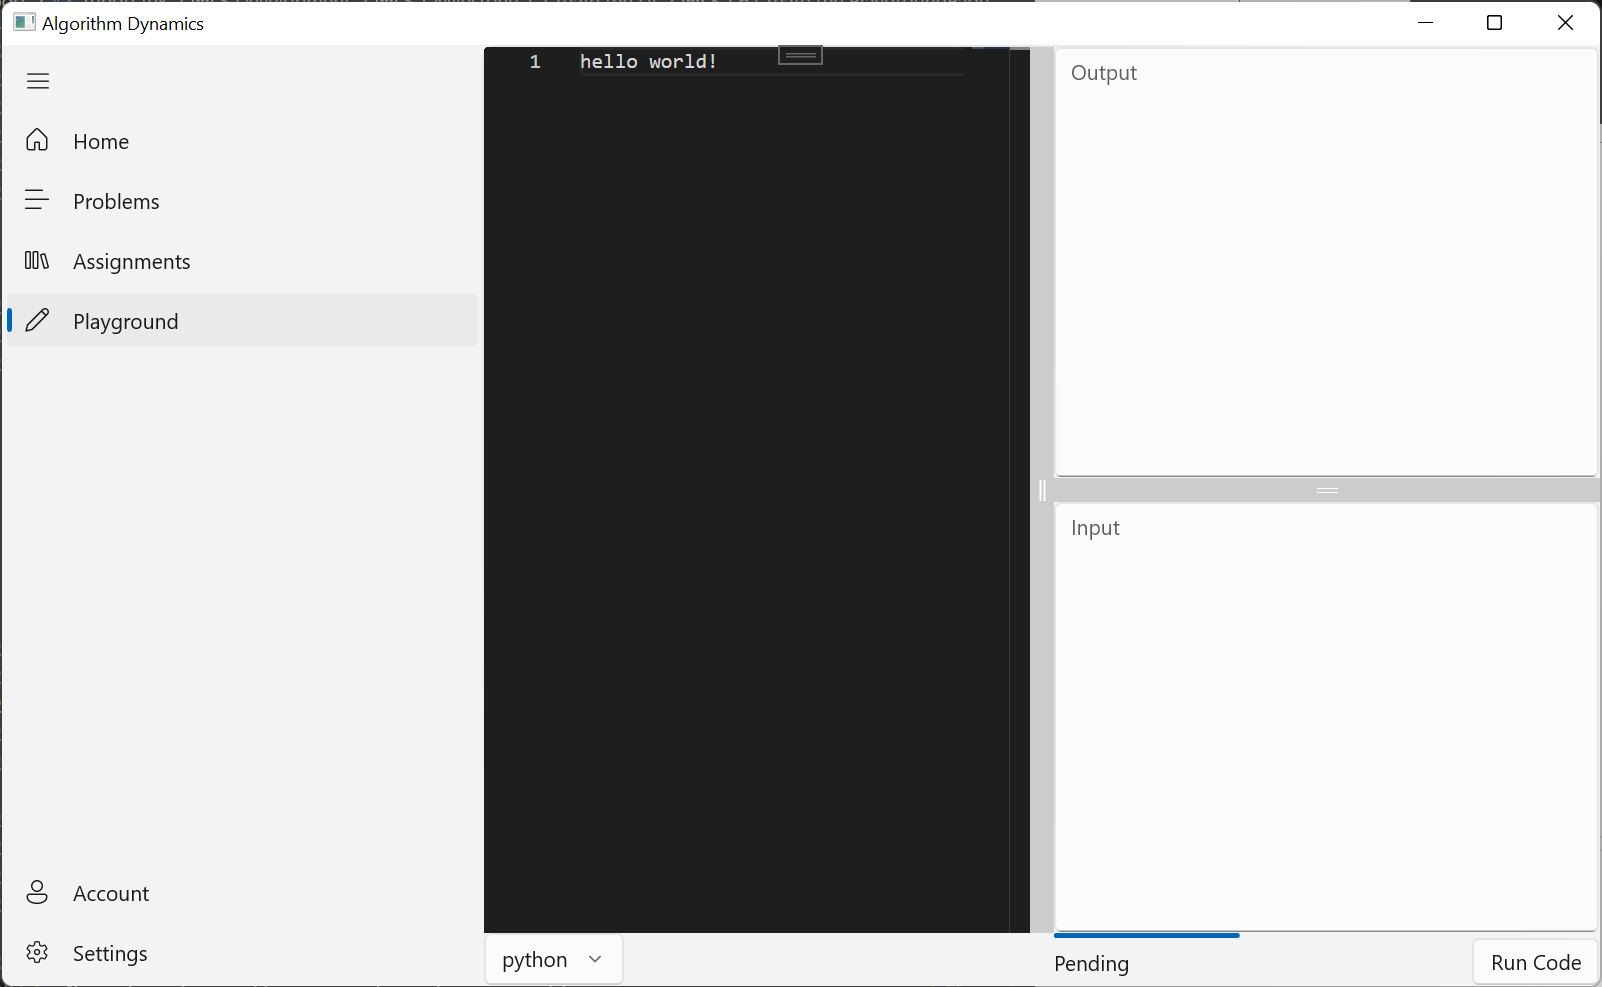
\includegraphics[width=\textwidth, height=\textheight, keepaspectratio]{PlaygroundPage-EditorConfig-Exposed}

Now when I run the app, it works correctly again.

I can pass config to the Monaco Editor now, but I also need to be able to retrieve the code input from the editor. To do this, I add an event listener to the editor, and post a web message when the code is changed.

\begin{minted}{javascript}
// Send code when the code is changed
window.editor.getModel().onDidChangeContent((e) => window.chrome.webview.postMessage(window.editor.getValue()))
\end{minted}

And on the app end, when I receive a new web message, I update the internal Code variable.

\begin{minted}{csharp}
/// <summary>
/// Update the Code when receive the value send by the Monaco Editor
/// </summary>
/// <param name="sender"></param>
/// <param name="args"></param>
private void CoreWebView2_WebMessageReceived(CoreWebView2 sender, CoreWebView2WebMessageReceivedEventArgs args)
{
    string data = args.TryGetWebMessageAsString();
    Code = data;
}

async void InitializeWebViewAsync()
{
    // ...
    WebView.CoreWebView2.WebMessageReceived += CoreWebView2_WebMessageReceived;
    // ...
}
\end{minted}

To test it is working, I bind the output box on the PlaygroundPage to CodeEditor.Code variable. When I type in the code editor, I should see the code in the output box updated with my typing.

\begin{minted}{xml}
<TextBox
    x:Name="OutputBox"
    Grid.Row="0"
    Grid.Column="1"
    Margin="8 0 0 8"
    PlaceholderText="Output"
    IsSpellCheckEnabled="False"
    AcceptsReturn="True"
    Text="{x:Bind CodeEditor.Code, Mode=OneWay}"/>
\end{minted}

When I run the app and start typing in the code editor, the output panel updates as expected, which means I have retrieved the code from the Monaco Editor successfully.

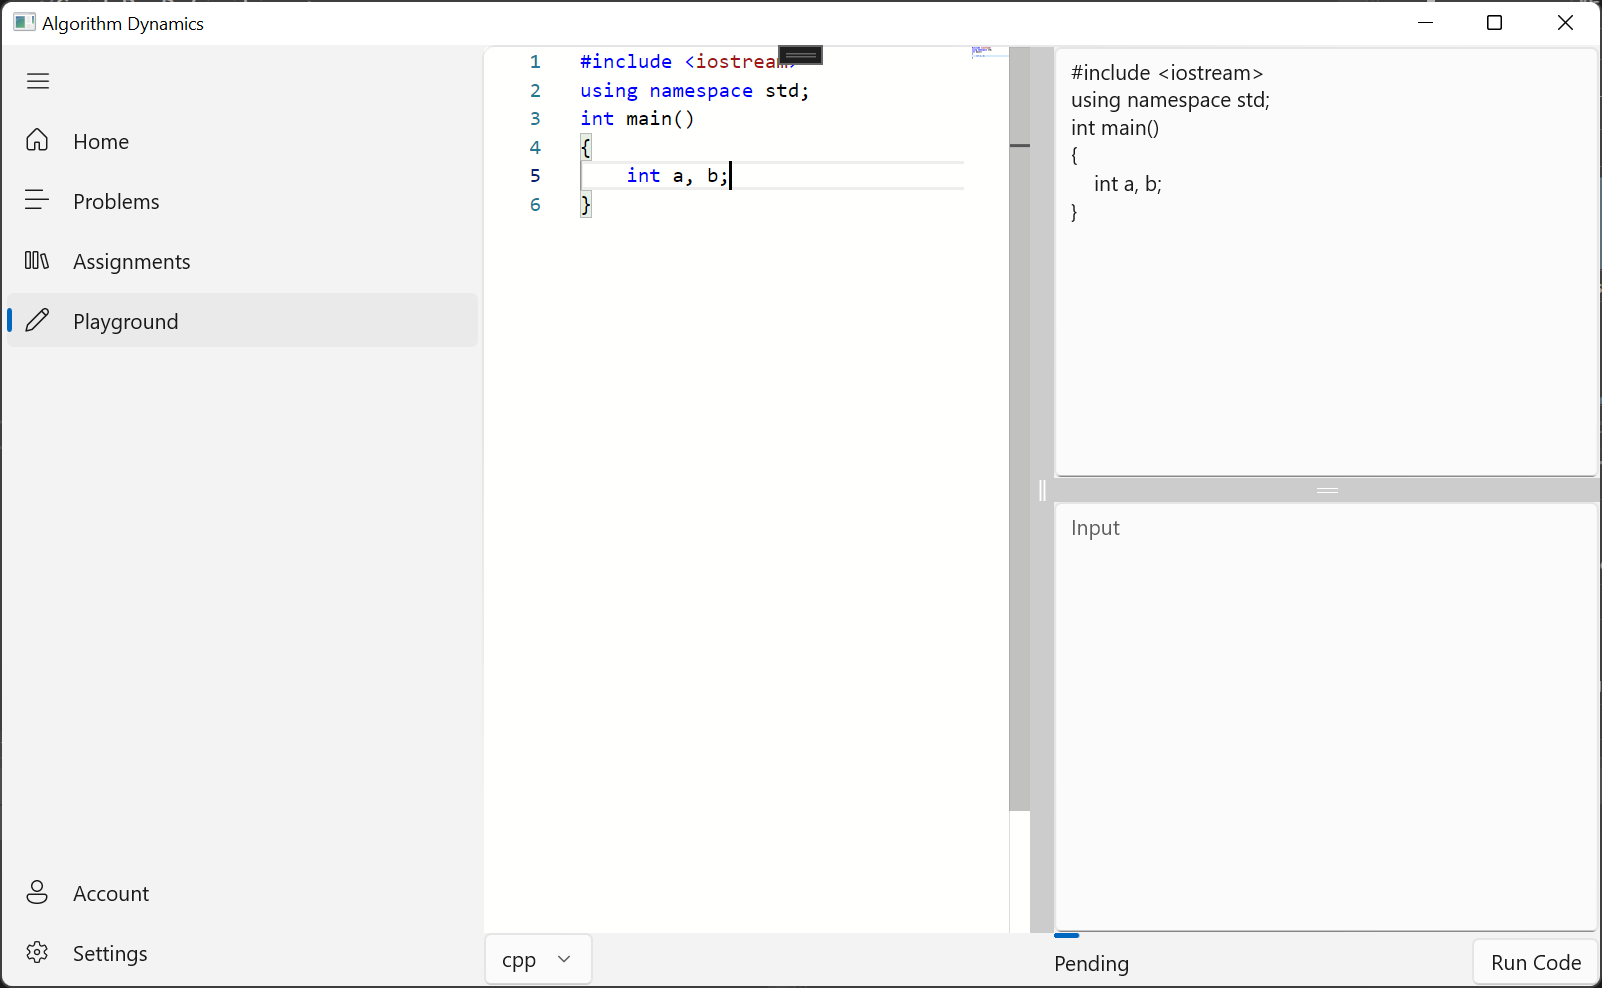
\includegraphics[width=\textwidth, height=\textheight, keepaspectratio]{PlaygroundPage-Editor-CodeSync}

I am not able to implement the full function of the PlaygroundPage right now since the Judger has not been implemented yet. But there is one last thing, I need to make the language ComboBox working. When the user selects a different programming, the syntax highlighting should adjust accordingly. This should be very easy to do since I have already implemented the config updaing function.

I add a new event handler to process the selection change event.

\begin{minted}{xml}
<ComboBox
    x:Name="LanguageComboBox"
    SelectedIndex="0"
    VerticalAlignment="Stretch"
    SelectionChanged="LanguageComboBox_SelectionChanged">
    <x:String>python</x:String>
    <x:String>c</x:String>
    <x:String>cpp</x:String>
    <x:String>javascript</x:String>
</ComboBox>
\end{minted}

And when I update the Lang variable, everything should just work.

\begin{minted}{csharp}
private void LanguageComboBox_SelectionChanged(object sender, SelectionChangedEventArgs e)
{
    CodeEditor.Lang = LanguageComboBox.SelectedItem.ToString();
}
\end{minted}

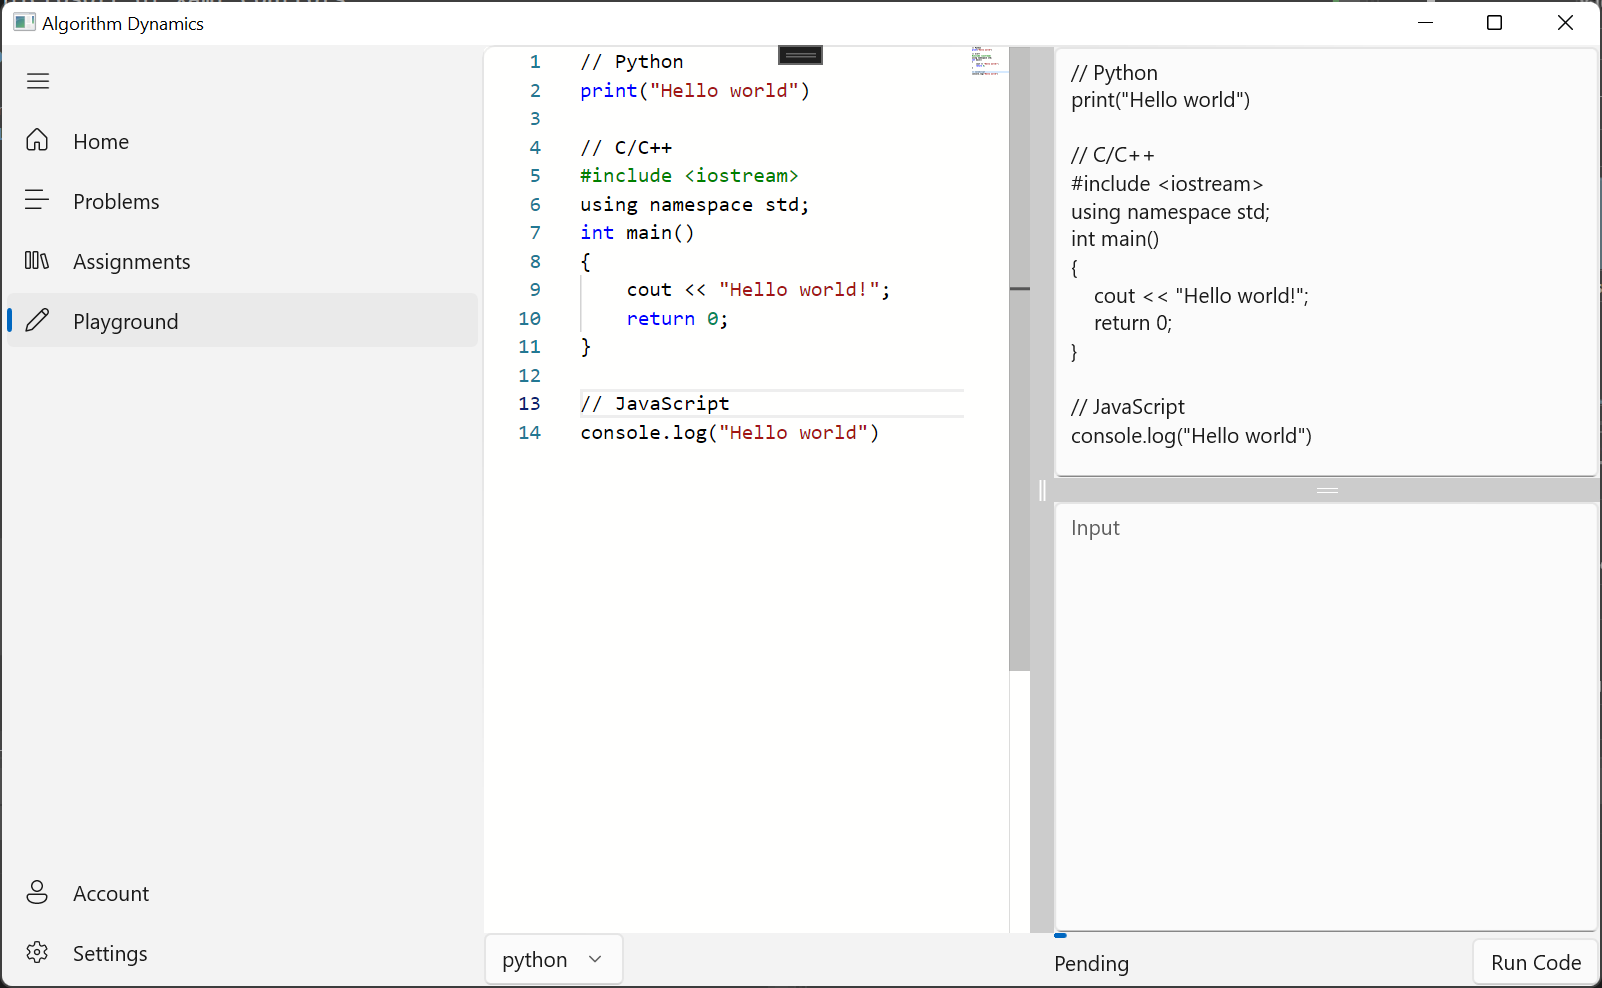
\includegraphics[width=\textwidth, height=\textheight, keepaspectratio]{PlaygroundPage-Editor-SyntaxHighlighting-Python}

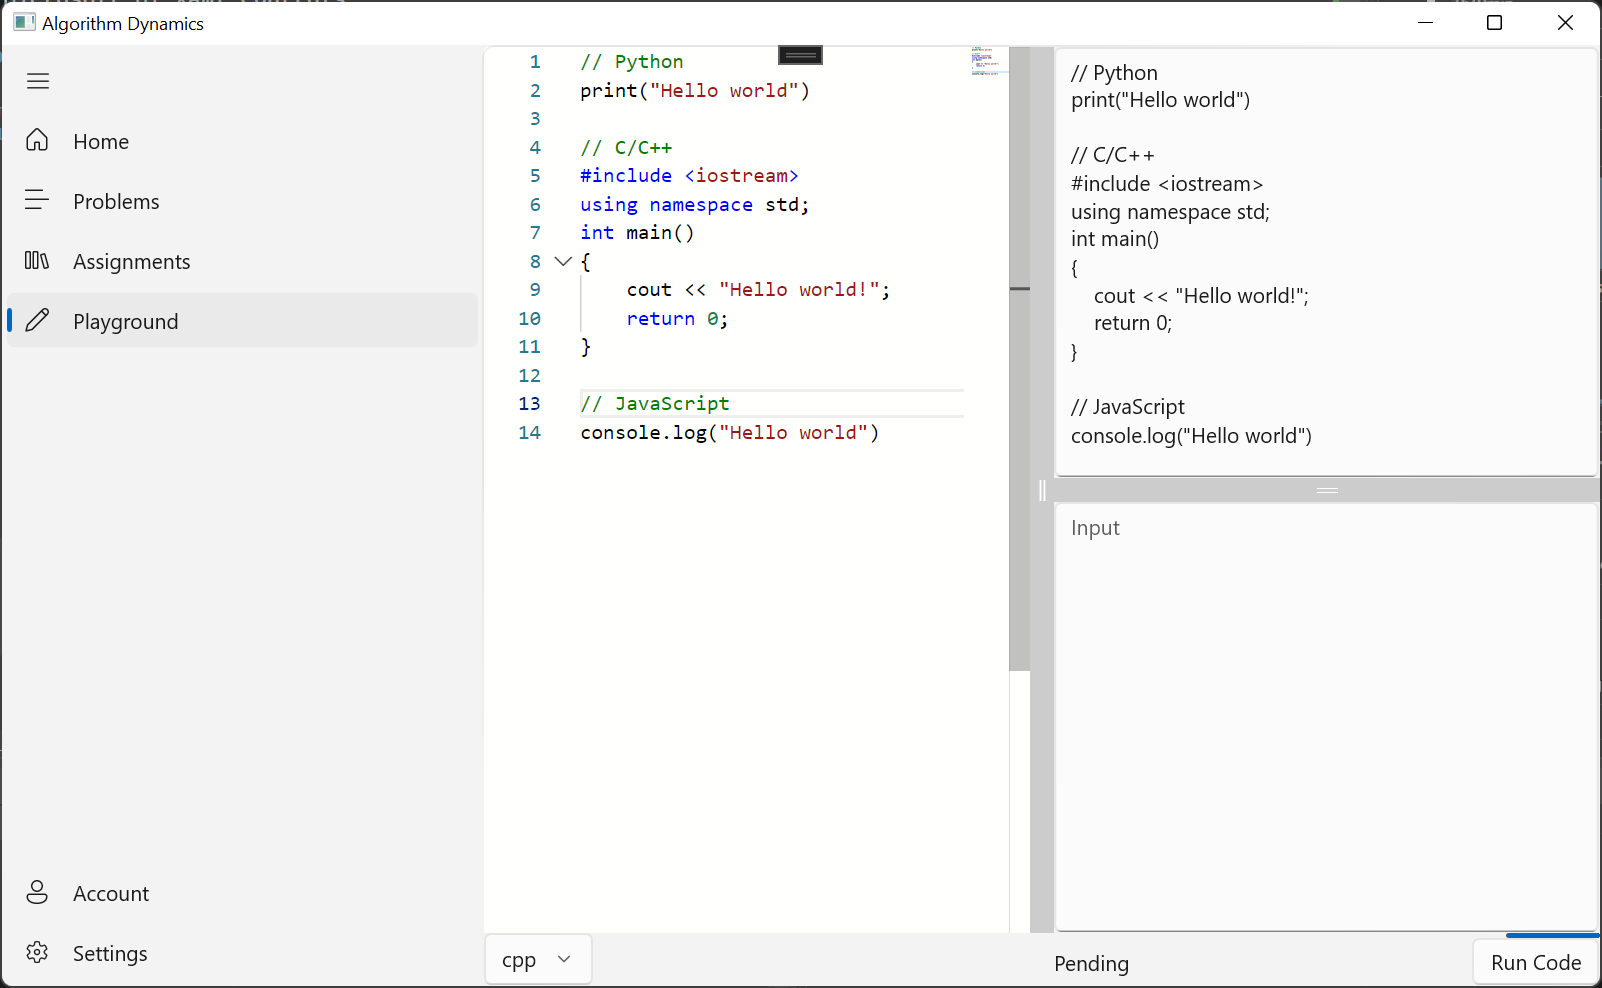
\includegraphics[width=\textwidth, height=\textheight, keepaspectratio]{PlaygroundPage-Editor-SyntaxHighlighting-Cpp}

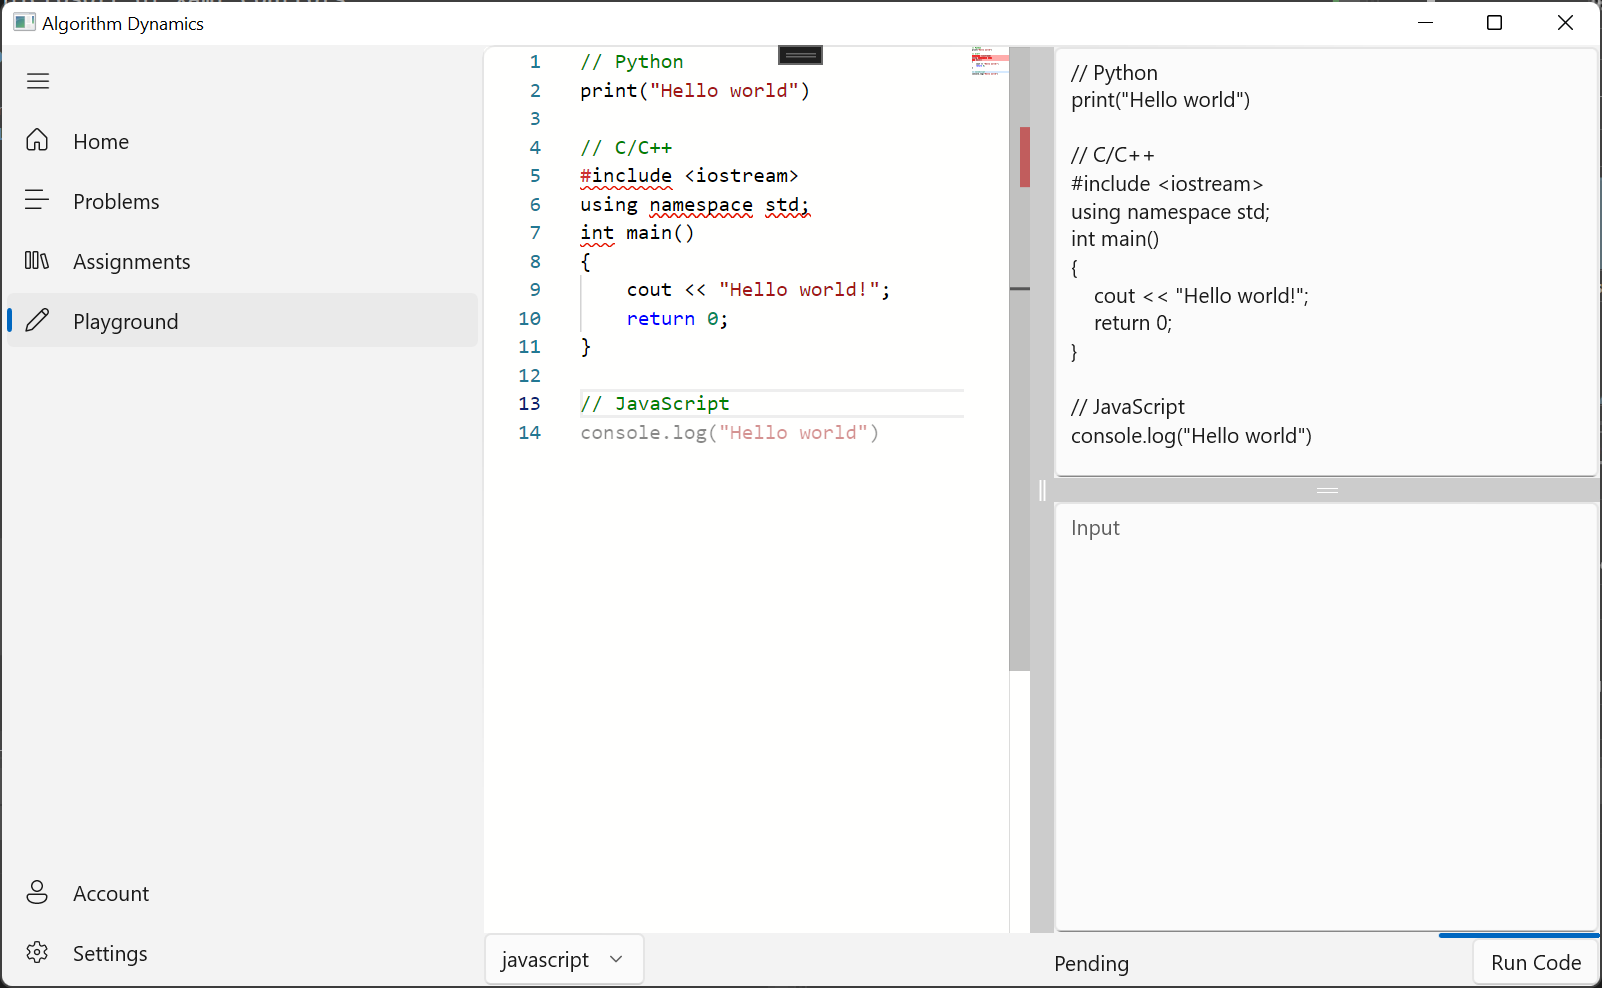
\includegraphics[width=\textwidth, height=\textheight, keepaspectratio]{PlaygroundPage-Editor-SyntaxHighlighting-JavaScript}

And it turns out to work perfectly as I expected. I can change the syntax highlighting in runtime smoothly.

I have finished the PlaygroundPage in this iteration. I will move on to the CodingPage next, which should be relatively simple because I have encapsulated the code editor into a user control and it can be easily reused.

Just before I plan to start the CodingPage, I find another bug with the Editor control. When the user navigate from the PlaygroundPage to another page, and then navigate back, the editor config cannot be loaded correctly. After some more research, it turns out that the WebView2 component is not destroyed after the page is unloaded, so when the next time it is loaded, it initialize much faster and load before \code{window.config} is set. I decide to design a three-way handshake protocol to solve this problem once and for all.

\includegraphics[width=\linewidth]{webviewHandshake}

At first, the WebView starts loading, and sends a message to request the initial configuration for the Monaco Editor when it is ready. The CodeEditor will keep listening until it receives the request. Then it will send the request and starts listening again. When the Monaco Editor is fully loaded, another message is sent to tell the CodeEditor it is ready. Then the initialization procedure is completed.

\begin{minted}{javascript}
require.config({ paths: { vs: 'monaco-editor/min/vs' } })
require(['vs/editor/editor.main'], () => {
    window.chrome.webview.postMessage('[Status] Request Configuration')
    window.chrome.webview.addEventListener('message', init)
})
function init() {
    // Remove the event listener
    window.chrome.webview.removeEventListener('message', init)
    // Initialize the code editor
    window.editor = monaco.editor.create(document.getElementById('container'), {
        value: window.config.Code,
        language: window.config.Language,
        theme: window.config.Theme
    })
    // Process resize event
    window.addEventListener("resize", () => window.editor.layout())
    // Send code when the code is changed
    window.editor.getModel().onDidChangeContent((e) => 
        window.chrome.webview.postMessage('[Data] ' + window.editor.getValue()))
    // Receive and set theme/language/code
    window.chrome.webview.addEventListener('message', (e) => {
        let data = e.data
        if (data.Theme) monaco.editor.setTheme(data.Theme)
        if (data.Language) monaco.editor.setModelLanguage(window.editor.getModel(), data.Language)
        if (data.Code) window.editor.getModel().setValue(data.Code)
    })
    // Ready
    window.chrome.webview.postMessage('[Status] Ready')
}
\end{minted}

For the CodeEditor control, I add a progress ring to display when it is going through the initilazation process.

\begin{minted}{xml}
<Grid>
    <WebView2 
        x:Name="WebView"
        HorizontalAlignment="Stretch"
        VerticalAlignment="Stretch"
        Visibility="Collapsed"/>
    <ProgressRing
        x:Name="ProgressRing"
        IsActive="True"
        HorizontalAlignment="Center"
        VerticalAlignment="Center"
        Visibility="Visible"/>
</Grid>
\end{minted}

\begin{minted}{csharp}
/// <summary>
/// Process the initialization process
/// Update the Code when receive the value send by the Monaco Editor
/// </summary>
/// <param name="sender"></param>
/// <param name="args"></param>
private async void CoreWebView2_WebMessageReceived(CoreWebView2 sender, CoreWebView2WebMessageReceivedEventArgs args)
{
    string data = args.TryGetWebMessageAsString();
    if (data == "[Status] Request Configuration")
    {
        EditorConfig editorConfig = new (GetTheme(RequestedTheme), Lang, Code);
        await WebView.ExecuteScriptAsync($"window.config={JsonSerializer.Serialize(editorConfig)}");
        WebView.CoreWebView2.PostWebMessageAsString("Configuration Sent");
    }
    else if (data == "[Status] Ready")
    {
        ProgressRing.Visibility = Visibility.Collapsed;
        WebView.Visibility = Visibility.Visible;
    } 
    else
    {
        // [Data] actual code
        Code = data.Substring("[Data] ".Length, data.Length - "[Data] ".Length);
        return;
    }
}
\end{minted}

Now, it is ok to navigate around different pages, and the editor will always be initialized correctly.

After testing the PlaygroundPage for a longer time, I find another issue. The memory usage of the app keep increasing each time when I navigate to and away from the PlaygroundPage. The memory garbage collection does not seem to work as expected. I suspect that is caused by the WebView2 control not being destroyed correctly. To verify my hypothesis, I use the Porcess Explorer \cite{microsoft:docs:process-explorer} to examine the process tree of the app.

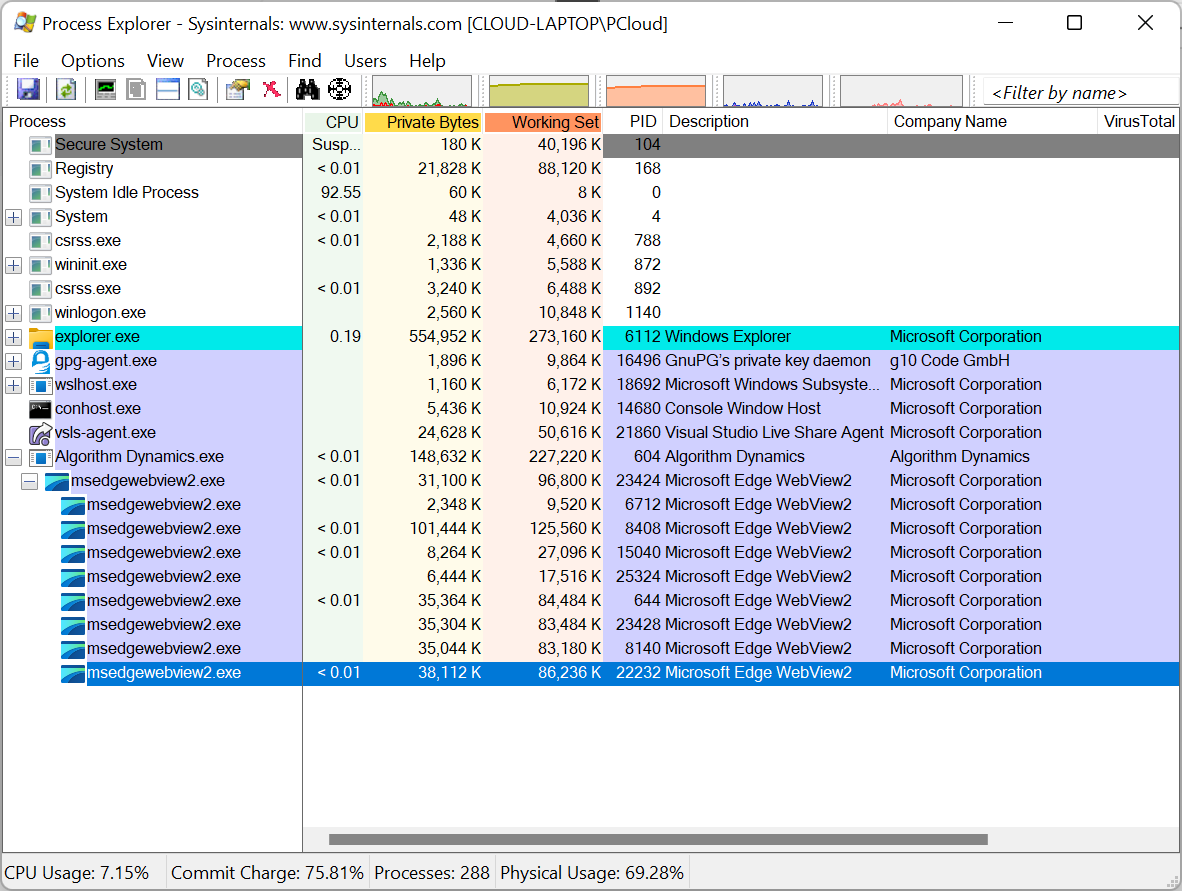
\includegraphics[width=\textwidth, height=\textheight, keepaspectratio]{Process-Explorer-WebView2}

As I expected, the WebView2 process is created not destroyed when I navigate away from the PlaygroundPage. And each time a new instance is create, which is causing the memory leak. After some researching on the lifecycle of the WebView2 component \cite{github:microsoft-ui-xaml:4752}, I found that I can call \code{WebView2.Close()} to manually dispose it. So I add a new procedure to handle the control unload event.

\begin{minted}{csharp}
private void CodeEditor_Unloaded(object sender, RoutedEventArgs e)
{
    // Close the WebView when unloaded
    // https://github.com/microsoft/microsoft-ui-xaml/issues/4752
    WebView.Close();
}
\end{minted}

Now, when I navigate away from the PlaygroundPage, I can see from the Process Explorer that all WebView2 processes are killed. And the memory usage fall back to the initial state correctly.

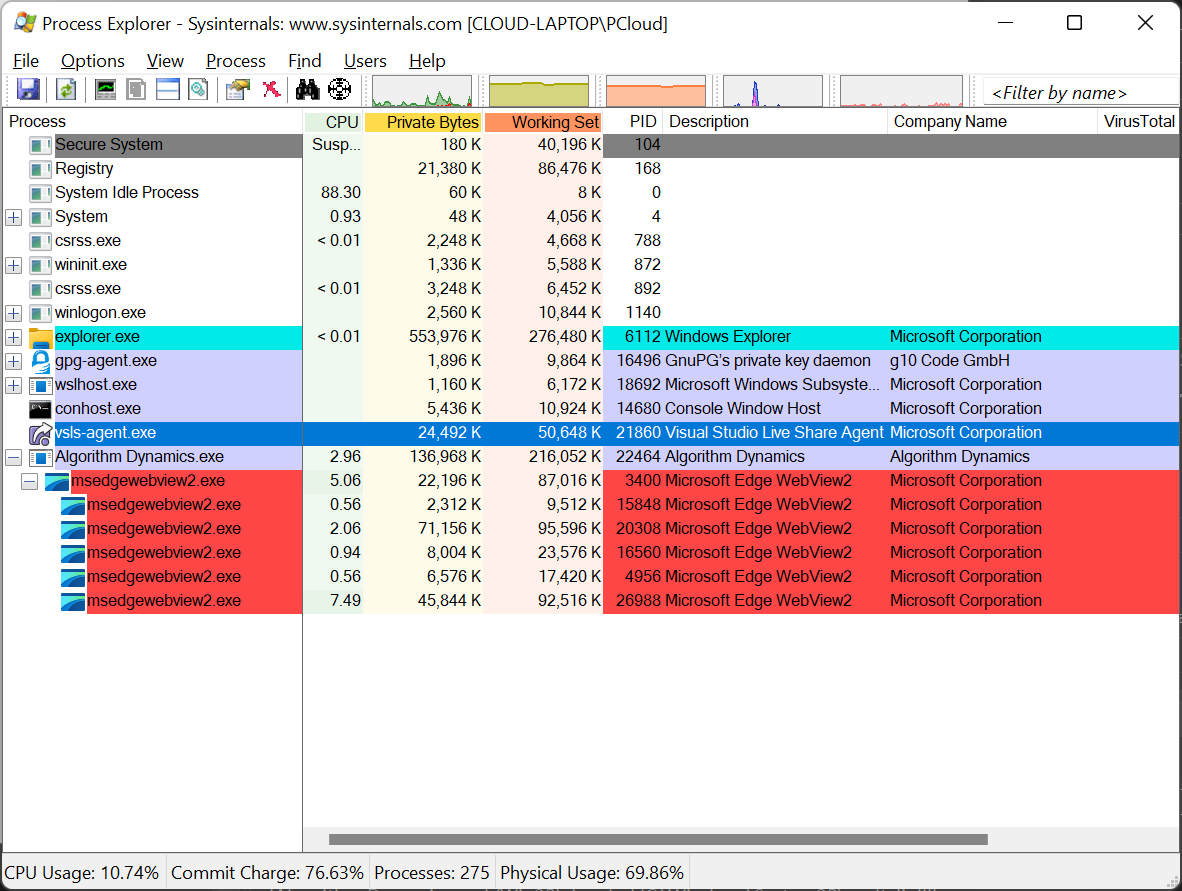
\includegraphics[width=\textwidth, height=\textheight, keepaspectratio]{Process-Explorer-WebView2-Destroyed}

\subsubsection{Testing and validation}

\begin{tabulary}{\linewidth}{|L|l|L|}
    \hline
    Test & Result & Remark \\
    \hline
    Does it load & Pass & \\
    \hline
    Can each section be resized correctly & Pass & \\
    \hline
    Does the CodeEditor work correctly & Pass & \\
    \hline
    Does the language ComboBox work correctly & Pass & \\
    \hline
    Does the input output box work correctly & Pass & \\
    \hline
    Does the Run Code button work & Failed & The Run Code function will be implemented after the Judger is ready. \\
    \hline
    Is the CodeEditor unloaded correctly on close & Pass & \\
    \hline
\end{tabulary}

\subsection{Create the CodingPage}

\subsubsection{Implementation}

I use a grid with 4 rows and 2 columns to organize all elements in the CodingPage.

\begin{minted}{xml}
<Page
    x:Class="Algorithm_Dynamics.Pages.CodingPage"
    xmlns="http://schemas.microsoft.com/winfx/2006/xaml/presentation"
    xmlns:x="http://schemas.microsoft.com/winfx/2006/xaml"
    xmlns:local="using:Algorithm_Dynamics.Controls"
    xmlns:controls="using:CommunityToolkit.WinUI.UI.Controls"
    xmlns:d="http://schemas.microsoft.com/expression/blend/2008"
    xmlns:mc="http://schemas.openxmlformats.org/markup-compatibility/2006"
    mc:Ignorable="d"
    Background="{ThemeResource ApplicationPageBackgroundThemeBrush}">
    <Grid>
        <Grid.RowDefinitions>
            <RowDefinition Height="auto"/>
            <RowDefinition Height="2*"/>
            <RowDefinition Height="*"/>
            <RowDefinition Height="auto"/>
        </Grid.RowDefinitions>

        <Grid.ColumnDefinitions>
            <ColumnDefinition Width="*"/>
            <ColumnDefinition Width="*"/>
        </Grid.ColumnDefinitions>

        <!-- ...  -->
</Page>
\end{minted}

I put a pivot on the top left, which holds two components, the MarkdownTextBlock for the description of the problem and the submission grid. The user can switch between them by clicking the pivot header.

\begin{minted}{xml}
<Pivot
    Grid.Row="0"
    Grid.RowSpan="3"
    Grid.Column="0"
    Margin="0 0 8 0">
    <PivotItem Header="Problem">
        <ScrollViewer
            HorizontalScrollBarVisibility="Disabled"
            VerticalScrollBarVisibility="Auto">
            <controls:MarkdownTextBlock
                x:Name="ProblemMarkdownTextBlock"
                Margin="8"
                Background="{ThemeResource ApplicationPageBackgroundThemeBrush}"
                Text="{x:Bind CodeEditor.Code, Mode=OneWay}"/>
        </ScrollViewer>
    </PivotItem>
    <PivotItem Header="Submissions">
        <controls:DataGrid
            x:Name="SubmissionsDataGrid"
            AutoGenerateColumns="True"
            ItemsSource="{x:Bind Submissions, Mode=OneWay}">
        </controls:DataGrid>
    </PivotItem>
</Pivot>
\end{minted}

I place the language selection box and the fullscreen button on the top right.

\begin{minted}{xml}
<Grid
    Grid.Row="0"
    Grid.Column="1"
    Margin="8">
    <Grid.ColumnDefinitions>
        <ColumnDefinition Width="*"/>
        <ColumnDefinition Width="*"/>
    </Grid.ColumnDefinitions>
    <ComboBox
        Grid.Column="0"
        x:Name="LanguageComboBox"
        SelectedIndex="0"
        VerticalAlignment="Stretch"
        SelectionChanged="LanguageComboBox_SelectionChanged">
        <x:String>python</x:String>
        <x:String>c</x:String>
        <x:String>cpp</x:String>
        <x:String>javascript</x:String>
    </ComboBox>
    <Button
        x:Name="FullScreenButton"
        Grid.Column="1"
        HorizontalAlignment="Right"
        Click="FullScreenButton_Click"
        ToolTipService.ToolTip="Fullscreen (F11)">
        <FontIcon
            x:Name="FullScreenIcon"
            FontFamily="Segoe Fluent Icons"
            Glyph="&#xE740;"/>
        <Button.KeyboardAccelerators>
            <KeyboardAccelerator Key="F11"/>
        </Button.KeyboardAccelerators>
    </Button>
</Grid>
\end{minted}

On the button right, I place the code editor and  Input/Output/Error panel inside another pivot so the user can navigate between them. Because the code editor has been encapsulated as a user control before, I can easily import it here.

\begin{minted}{xml}
<local:CodeEditor
    x:Name="CodeEditor"
    Grid.Column="1"
    Grid.Row="1"
    Margin="8 0 0 8"/>
<Pivot
    Grid.Row="2"
    Grid.Column="1"
    Margin="8 8 0 0">
    <PivotItem Header="Input">
        <TextBox
            x:Name="InputTextBox"
            x:FieldModifier="public"
            PlaceholderText="Input Panel"
            AcceptsReturn="True"/>
    </PivotItem>
    <PivotItem Header="Output">
        <TextBox
            x:Name="OutputTextBox"
            x:FieldModifier="public"
            PlaceholderText="Output Panel"
            AcceptsReturn="True"/>
    </PivotItem>
    <PivotItem Header="Error">
        <TextBox
            x:Name="ErrorTextBox"
            x:FieldModifier="public"
            PlaceholderText="Error Panel"
            AcceptsReturn="True"/>
    </PivotItem>
</Pivot>
\end{minted}

At the bottom, I place the problem navigation buttons, the status text block, a progress bar and the run code and submission button.

\begin{minted}{xml}
<Grid
    Grid.Row="3"
    Grid.Column="1">
    <Grid.RowDefinitions>
        <RowDefinition Height="auto"/>
        <RowDefinition Height="*"/>
    </Grid.RowDefinitions>
    
    <Grid.ColumnDefinitions>
        <ColumnDefinition Width="*"/>
        <ColumnDefinition Width="auto"/>
        <ColumnDefinition Width="auto"/>
    </Grid.ColumnDefinitions>

    <ProgressBar
        Grid.Row="0"
        Grid.Column="0"
        Grid.ColumnSpan="3"
        IsIndeterminate="True"
        ShowPaused="False"
        ShowError="False"/>
    <TextBlock
        Grid.Row="1"
        Grid.Column="0"
        Text="Status"
        VerticalAlignment="Center"/>
    <Button
        Grid.Row="1"
        Grid.Column="2"
        x:Name="SubmitCodeButton"
        Content="Submit"
        Style="{StaticResource AccentButtonStyle}"/>
    <Button
        Grid.Row="1"
        Grid.Column="1"
        Content="Run Code"/>
</Grid>

<Grid
    Grid.Row="3"
    Grid.Column="0">
    <Grid.ColumnDefinitions>
        <ColumnDefinition Width="auto"/>
        <ColumnDefinition Width="auto"/>
        <ColumnDefinition Width="auto"/>
    </Grid.ColumnDefinitions>
    <Button
        Grid.Column="0"
        VerticalAlignment="Stretch">
        <Button.Content>
            <FontIcon FontFamily="Segoe Fluent Icons" Glyph="&#xE76B;"/>
        </Button.Content>
    </Button>
    <DropDownButton
        Grid.Column="1"
        Content="Problem 0"
        VerticalAlignment="Stretch">
        <DropDownButton.Flyout>
            <MenuFlyout Placement="Top">
                <MenuFlyoutItem Text="Problem 1"/>
                <MenuFlyoutItem Text="Problem 2"/>
                <MenuFlyoutItem Text="Problem 3"/>
            </MenuFlyout>
        </DropDownButton.Flyout>

    </DropDownButton>
    <Button
        Grid.Column="2"
        VerticalAlignment="Stretch">
        <Button.Content>
            <FontIcon FontFamily="Segoe Fluent Icons" Glyph="&#xE76C;"/>
        </Button.Content>
    </Button>
</Grid>
\end{minted}

At the end, I add two grid splitters between the problem panel and the editor, the editor and the panel so users can resize each window to fit their needs.

When I build and run the app, I encounter a problem - I cannot navigate to the CodingPage. Unlike the previous pages, the CodingPage is not a top-level page, it is opened when the user select a problem or an assignment. So I need to link the start problem button to the CodingPage. So for the Start button on the ProblemsPage, I add a StartProblem function to handle the click event.

\begin{minted}{xml}
<Button
    Content="Start"
    Grid.Column="4"
    HorizontalAlignment="Stretch"
    Margin="12 0 0 0"
    Click="StartProblem"/>
\end{minted}

\begin{minted}{csharp}
/// <summary>
/// Navigate to the CodingPage, pass the current Problem and ProblemList
/// </summary>
/// <param name="sender"></param>
/// <param name="e"></param>
private void StartProblem(object sender, RoutedEventArgs e)
{
    App app = (App)Application.Current;
    // TODO pass the selected problem to the CodingPage
    app.ContentFrame.Navigate(typeof(CodingPage));
    app.MainNavView.SelectedItem = null;
}
\end{minted}

The function should also pass the selected problem and the problem list through the Navigate function. But since the data structure is not implemented, for now, it just navigates to the page without passing any data.

Now when I run the app, I can navigate to the CodingPage through the ProblemsPage and see all the layout I defined before.

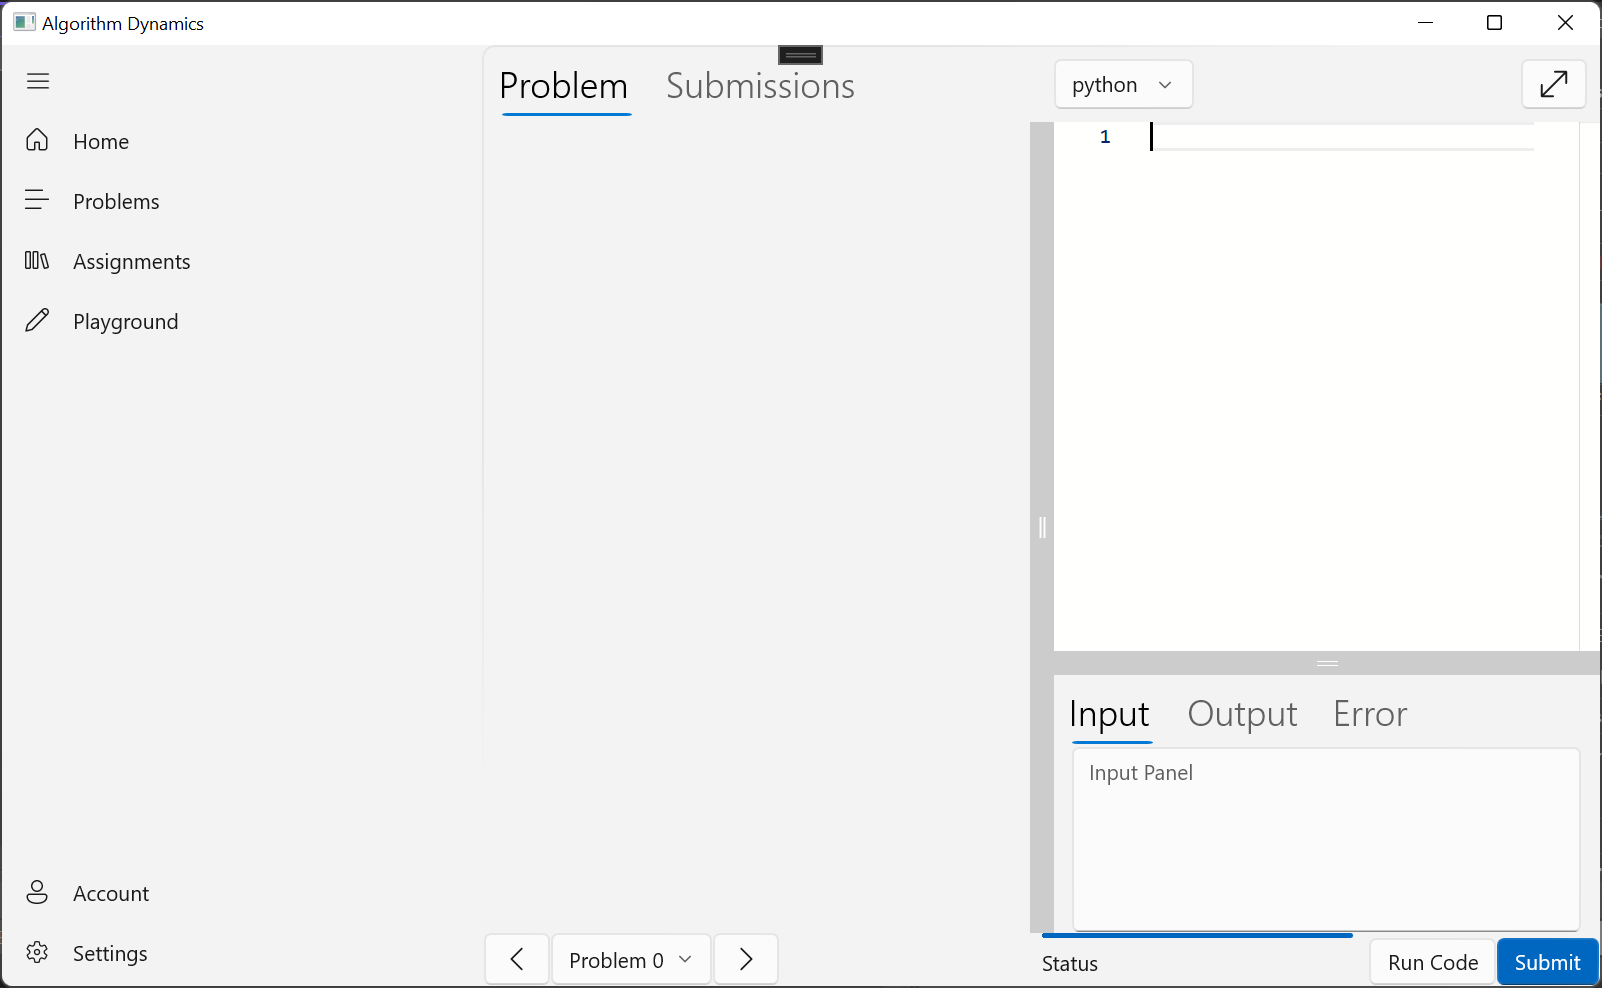
\includegraphics[width=\textwidth, height=\textheight, keepaspectratio]{CodingPage-Layout}

When I provide the screenshot to my stakeholder PCloud, he says that the controls are quite ugly, especially the pivot and the grid splitter, the font and color theme does not seem to match the overall design. I agree with him, so I decide to add some style to the pivot and the grid splitter.

I create a new file Generic.xaml to store all the styles. In App.xaml, I import the Generic.xaml file.

\begin{minted}{xml}
<Application.Resources>
    <ResourceDictionary>
        <ResourceDictionary.MergedDictionaries>
            <XamlControlsResources xmlns="using:Microsoft.UI.Xaml.Controls" />
            <ResourceDictionary Source="/Themes/Generic.xaml"/>
            <!-- Other merged dictionaries here -->
        </ResourceDictionary.MergedDictionaries>
        <!-- Other app resources here -->
    </ResourceDictionary>
</Application.Resources>
\end{minted}

For the GridSplitter, I reference the design in DevToys\cite{github:DevToys:Generic.xaml} by setting the background color to transparent which makes the GridSplitter less significant.

For the Pivot, I reference the design from the Windows Calculator\cite{github:calculator:Calculator.xaml}, which modifies the Pivot to make it look like the modern NavigationView.

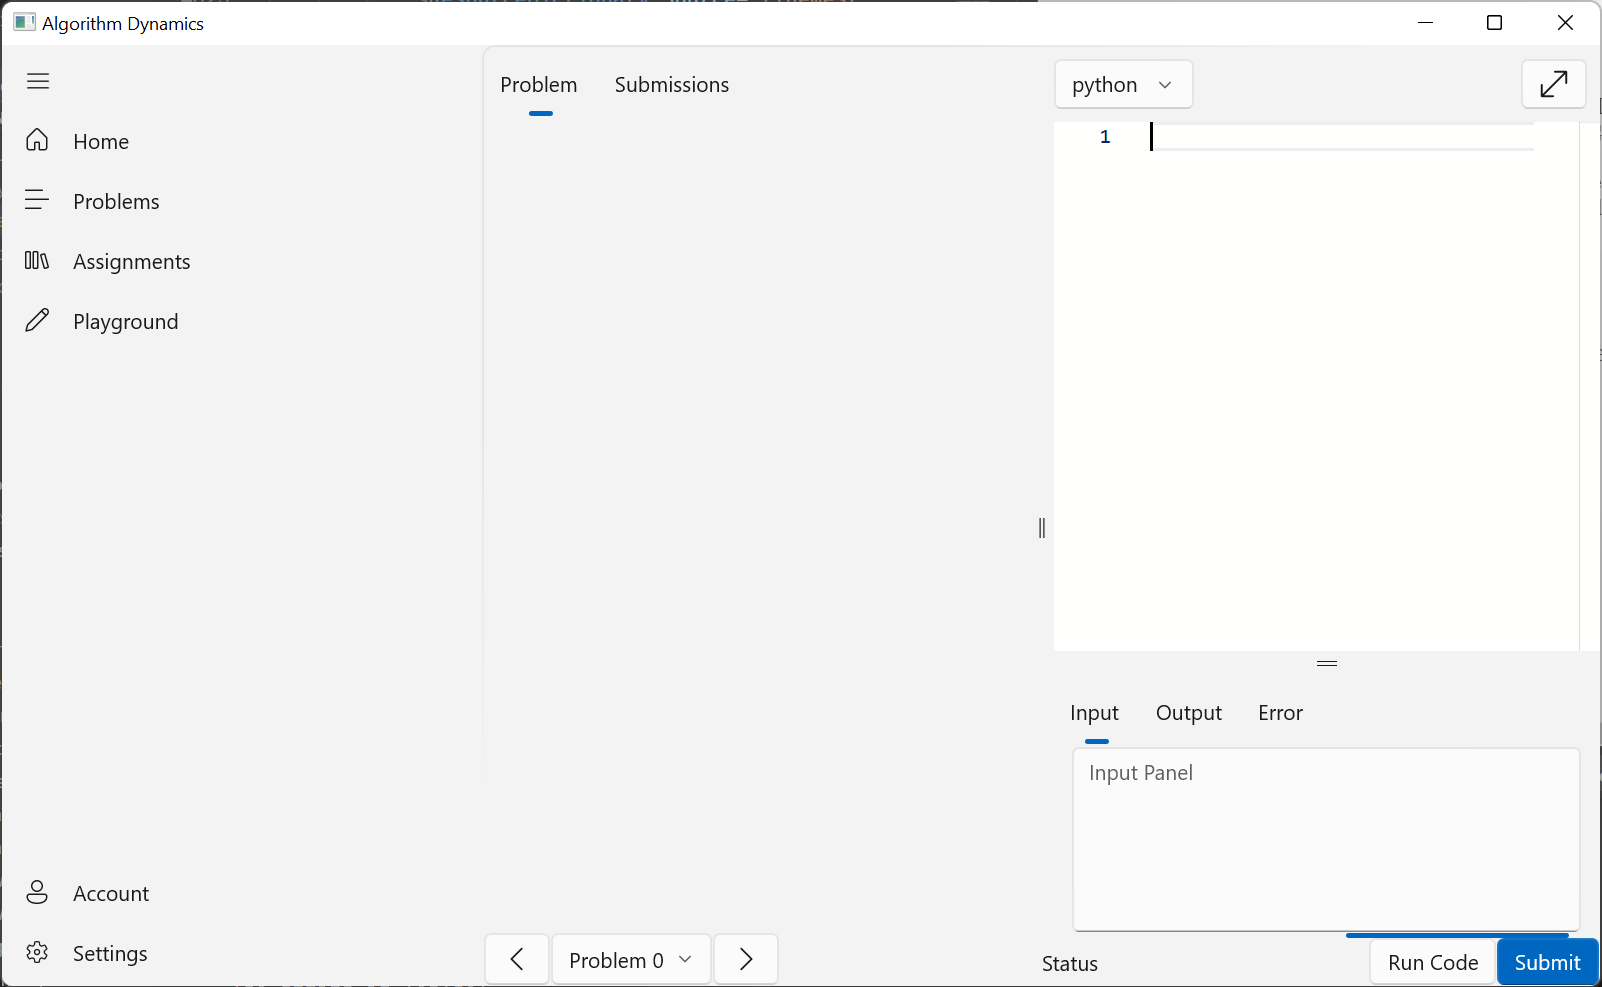
\includegraphics[width=\textwidth, height=\textheight, keepaspectratio]{CodingPage-Theme}

After applying the custom theme, the interface looks much more modern and consistent.

Next I will implement the full screen button. It will be a toggle, when clicking in the window mode, it set the window to full screen. When clicking in the full screen mode, it sets the window back to a window. I also assigned a keyboard accelerator F11 to the button, so the user can toggle it by keyboard.

\begin{minted}{xml}
<Button
    x:Name="FullScreenButton"
    Grid.Column="1"
    HorizontalAlignment="Right"
    Click="FullScreenButton_Click"
    ToolTipService.ToolTip="Fullscreen (F11)">
    <FontIcon
        x:Name="FullScreenIcon"
        FontFamily="Segoe Fluent Icons"
        Glyph="&#xE740;"/>
    <Button.KeyboardAccelerators>
        <KeyboardAccelerator Key="F11"/>
    </Button.KeyboardAccelerators>
</Button>
\end{minted}

In the \code{FullScreenButton_Click} function, I implement the logic of the toggle button. It sets the \code{AppWindowPresent} property\cite{microsoft:docs:windowing-overview} to the opposite value and assign the correct icon\cite{microsoft:docs:segoe-fluent-icons-font}.

\begin{minted}{csharp}
/// <summary>
/// Toggle the fullscreen mode for the app
/// Toggle the <see cref="AppWindowPresenterKind"/> and <see cref="FullScreenIcon.Glyph"/>
/// </summary>
/// <param name="sender"></param>
/// <param name="e"></param>
private void FullScreenButton_Click(object sender, RoutedEventArgs e)
{
    AppWindow window = MainWindow.AppWindow;
    if (window.Presenter.Kind == AppWindowPresenterKind.Overlapped)
    {
        window.SetPresenter(AppWindowPresenterKind.FullScreen);
        FullScreenIcon.Glyph = "\xE73F";
    }
    else
    {
        window.SetPresenter(AppWindowPresenterKind.Overlapped);
        FullScreenIcon.Glyph = "\xE740";
    }
}
\end{minted}

Now when I click the button, it does go into the fullscreen mode with the correct button icon set. But I notice that the system taskbar is blank instead of filled with the app window. After doing some research, it turns out that this is caused by an internal bug of the WindowsAppSDK\cite{github:WindowsAppSDK:1853} and I cannot fix it on my side. I will just leave it like this until a new version of the SDK is released.

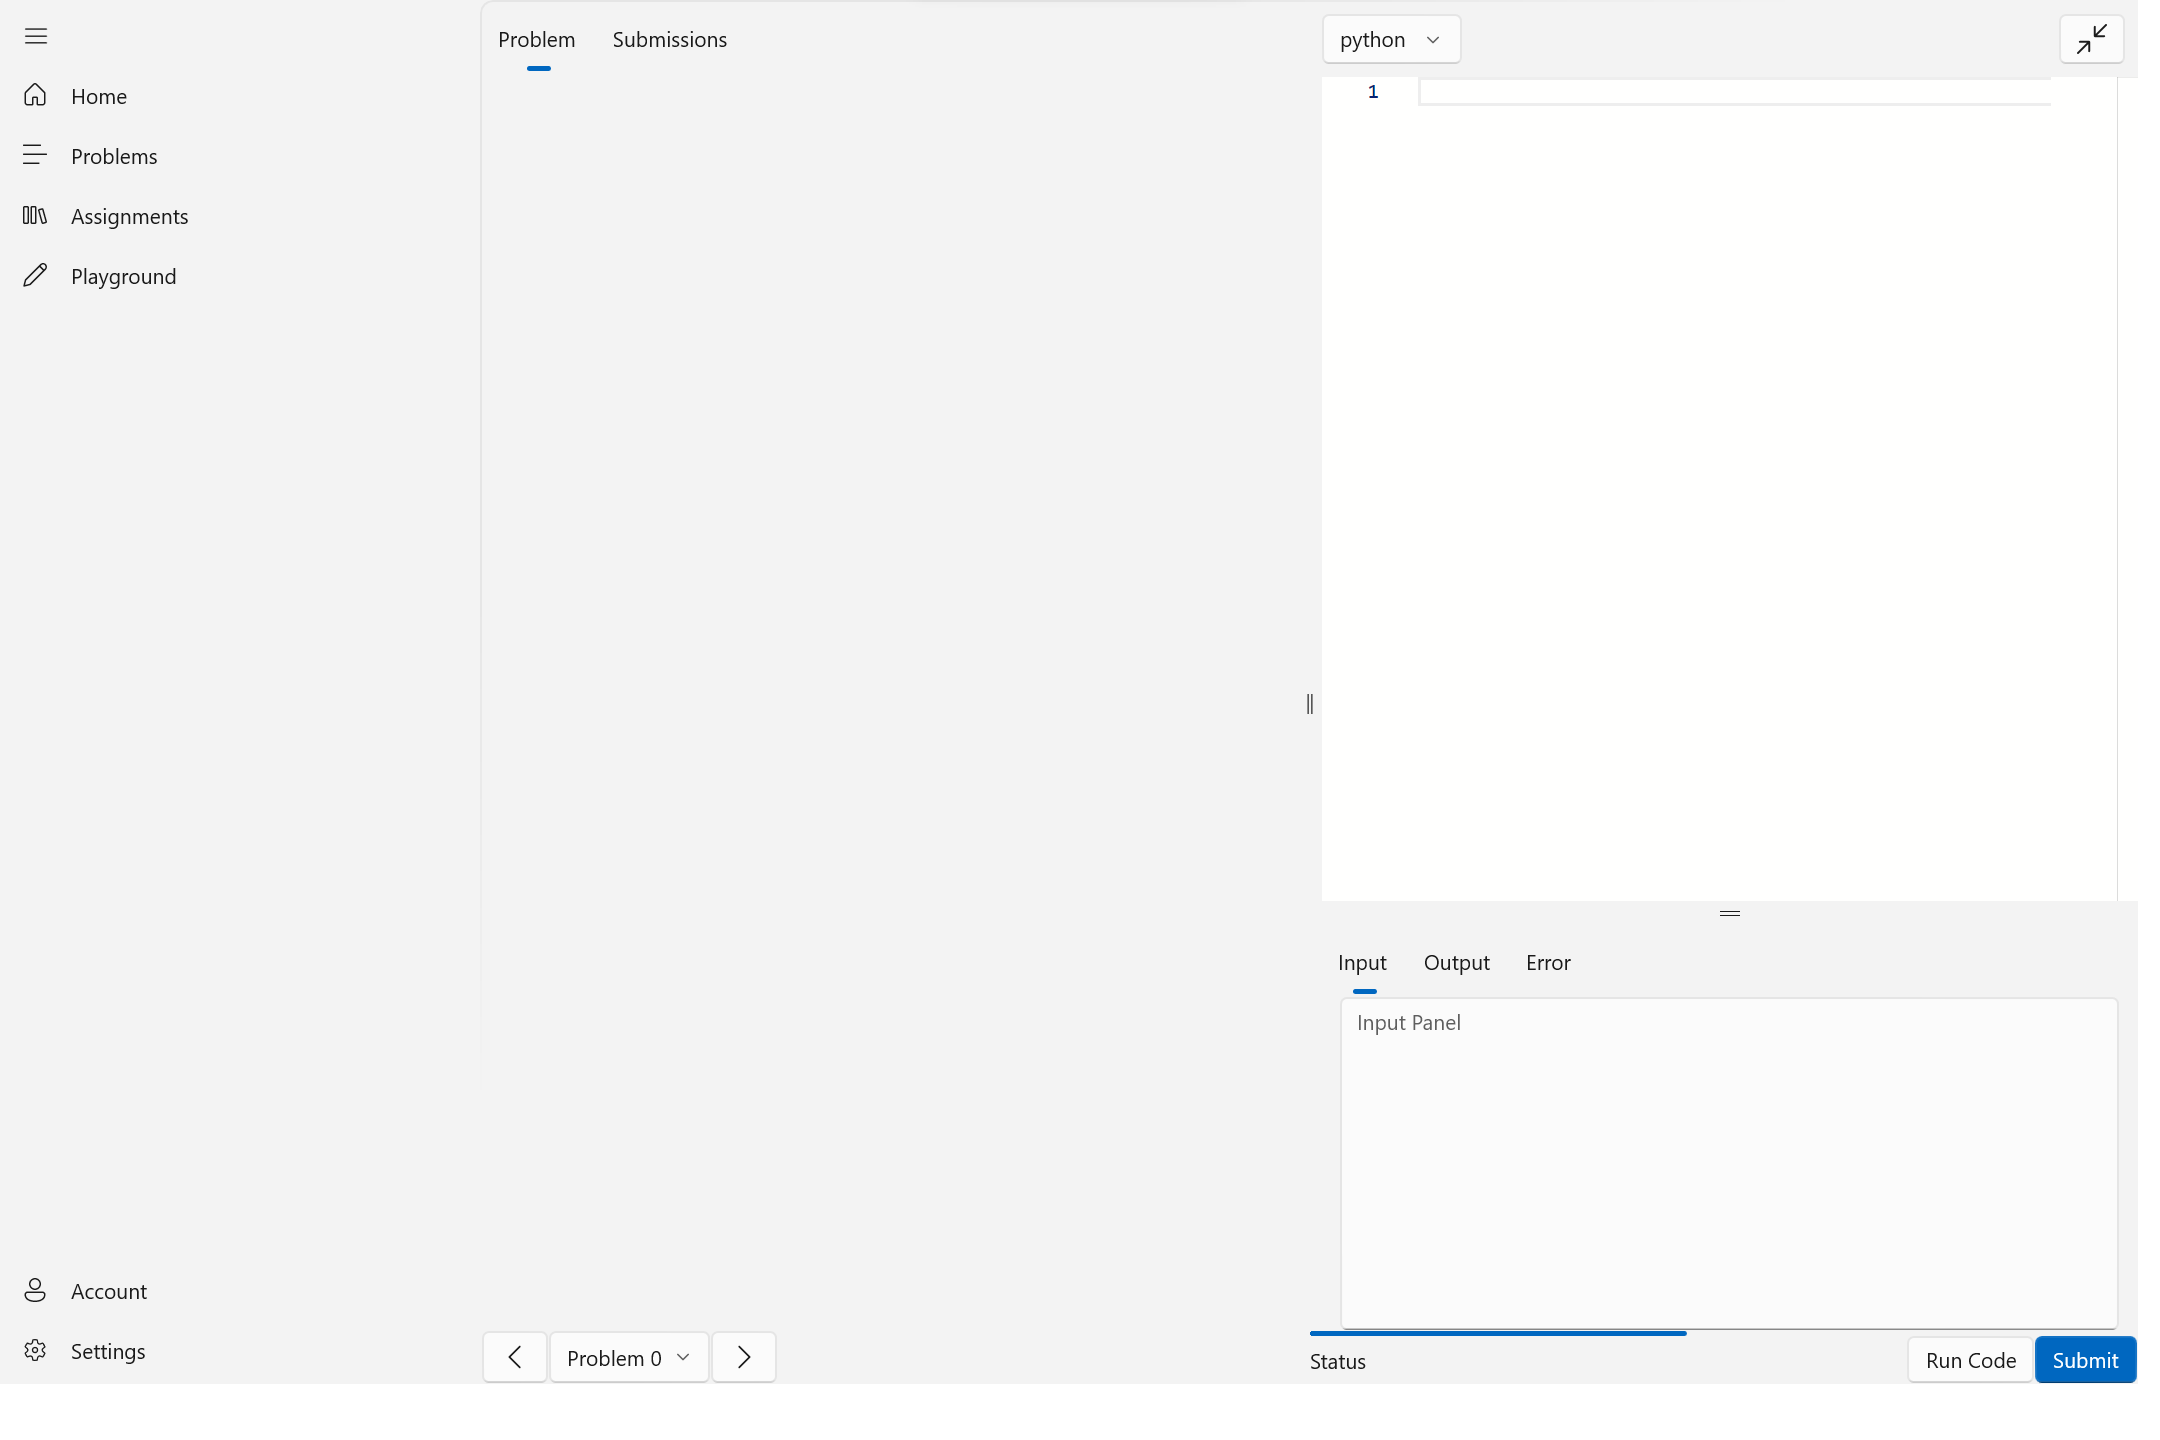
\includegraphics[width=\textwidth, height=\textheight, keepaspectratio]{CodingPage-FullScreen-Bug.png}

For the other parts, the submission records depend on the database, and the run code and submit function depends on the Judger, so in this iteration, I will leave the page like this.

\subsubsection{Testing and validation}

\begin{tabulary}{\linewidth}{|L|l|L|}
    \hline
    Test & Result & Remark \\
    \hline
    Does it load & Failed & This feature is not fully implemented. When the CodingPage loads, it should take in two parameter, the current problem and a problem list for navigation. The main page can load correctly, but the support for these two parameters are not yet implemented because the data structure is not implemented yet. \\
    \hline
    Does the full screen button work & Pass & \\
    \hline
    Does the markdown text block work & Pass & \\
    \hline
    Does the code editor work & Pass & \\
    \hline
    Does the input panel work & Pass & \\
    \hline
    Does the output panel work & Pass & \\
    \hline
    Does the error panel work & Pass & \\
    \hline
    Does the language selection box work & Pass & \\
    \hline
    Does the Run Code button work & Failed & Not implemented because the Judger is not ready. \\
    \hline
    Does the Submit button work & Failed & Not implemented because the Judger is not ready. \\
    \hline
    Does the Submit problem navigation & Failed & Not implemented because the data structure is not ready. \\
    \hline
    Does the submission history table work & Failed & Not implemented because the database is not ready. \\
    \hline
\end{tabulary}

\subsection{Create the AccountPage}

\subsubsection{Implementation}

For the AccountPage, I use a grid of two row to divide the two sections for the account information and the statistics data. For the account information, I decide to use the RelativePanel to construct the layout to make it responsive to different sizes of the window. For the statistics data, I use the AdaptiveGridView which is used for the HomePage as well, so the data can be dynamically added in the code behind and make it a lot easier to add custom statistics later.

\begin{minted}{xml}
<Grid>
    <Grid.RowDefinitions>
        <RowDefinition Height="*"/>
        <RowDefinition Height="*"/>
    </Grid.RowDefinitions>

    <RelativePanel
        Grid.Row="0"
        HorizontalAlignment="Stretch"
        VerticalAlignment="Stretch">
        <PersonPicture
            x:Name="AvatarPicture"
            Margin="32"
            RelativePanel.AlignLeftWithPanel="True"
            RelativePanel.AlignVerticalCenterWithPanel="True"
            ProfilePicture="https://docs.microsoft.com/windows/uwp/contacts-and-calendar/images/shoulder-tap-static-payload.png" />
        <StackPanel
            RelativePanel.RightOf="AvatarPicture"
            RelativePanel.AlignVerticalCenterWithPanel="True">
            <TextBlock
                Margin="2"
                Text="Name"
                Style="{ThemeResource SubtitleTextBlockStyle}"/>
            <TextBlock
                Margin="2"
                Text="Email"
                Style="{ThemeResource BodyTextBlockStyle}"/>
            <TextBlock
                Margin="2"
                Text="Role"
                Style="{ThemeResource BodyTextBlockStyle}"/>
        </StackPanel>
        <StackPanel
            Margin="32"
            RelativePanel.AlignRightWithPanel="True"
            RelativePanel.AlignVerticalCenterWithPanel="True">
            <Button
                Margin="2"
                HorizontalAlignment="Stretch"
                Content="Edit"/>
            <Button
                Margin="2"
                HorizontalAlignment="Stretch"
                Content="Login"/>
        </StackPanel>
    </RelativePanel>

    <controls:AdaptiveGridView
        x:Name="StatsGridView"
        Grid.Row="1"
        Margin="0"
        ItemsSource="{x:Bind StatsItems}"
        StretchContentForSingleRow="False"
        OneRowModeEnabled="False"
        ItemHeight="120"
        DesiredWidth="240"
        SelectionMode="None"
        IsItemClickEnabled="False"
        Background="{ThemeResource AcrylicBackgroundFillColorDefaultBrush}">
        <GridView.ItemTemplate>
            <DataTemplate x:DataType="models:StatisticsItem">
                <Grid HorizontalAlignment="Stretch">
                    <StackPanel 
                        VerticalAlignment="Center"
                        HorizontalAlignment="Center"
                        Orientation="Vertical"
                        Margin="8">
                        <TextBlock
                            Text="{x:Bind Title}"
                            Margin="2"
                            Style="{ThemeResource BodyStrongTextBlockStyle}"
                            HorizontalAlignment="Center"/>
                        <TextBlock 
                            Text="{x:Bind Data}"
                            Margin="2"
                            HorizontalAlignment="Center"/>
                    </StackPanel>
                </Grid>
            </DataTemplate>
        </GridView.ItemTemplate>
    </controls:AdaptiveGridView>

</Grid>
\end{minted}

Similar to the HomePage, I create a model \code{StatisticsItem} for the statistics data and binds it to the grid. For now, I just add some sample data in for display purpose.

\begin{minted}{csharp}
public class StatisticsItem
{
    public StatisticsItem(string title, string data)
    {
        Title = title;
        Data = data;
    }

    public string Title { get; set; }
    public string Data { get; set; }
}
\end{minted}

\begin{minted}{csharp}
public AccountPage()
{
    InitializeComponent();
    StatsItems.Add(new StatisticsItem("Problem Solved", "10"));
    StatsItems.Add(new StatisticsItem("Problem Attempted", "3"));
    StatsItems.Add(new StatisticsItem("Problem Unsolved", "1100"));
    StatsItems.Add(new StatisticsItem("Correct Rate", "10%"));
    StatsItems.Add(new StatisticsItem("Favourite Topic", "Data structure"));
    StatsItems.Add(new StatisticsItem("Favourite Language", "Python"));
}
public ObservableCollection<StatisticsItem> StatsItems { get; } = new ObservableCollection<StatisticsItem>();
\end{minted}

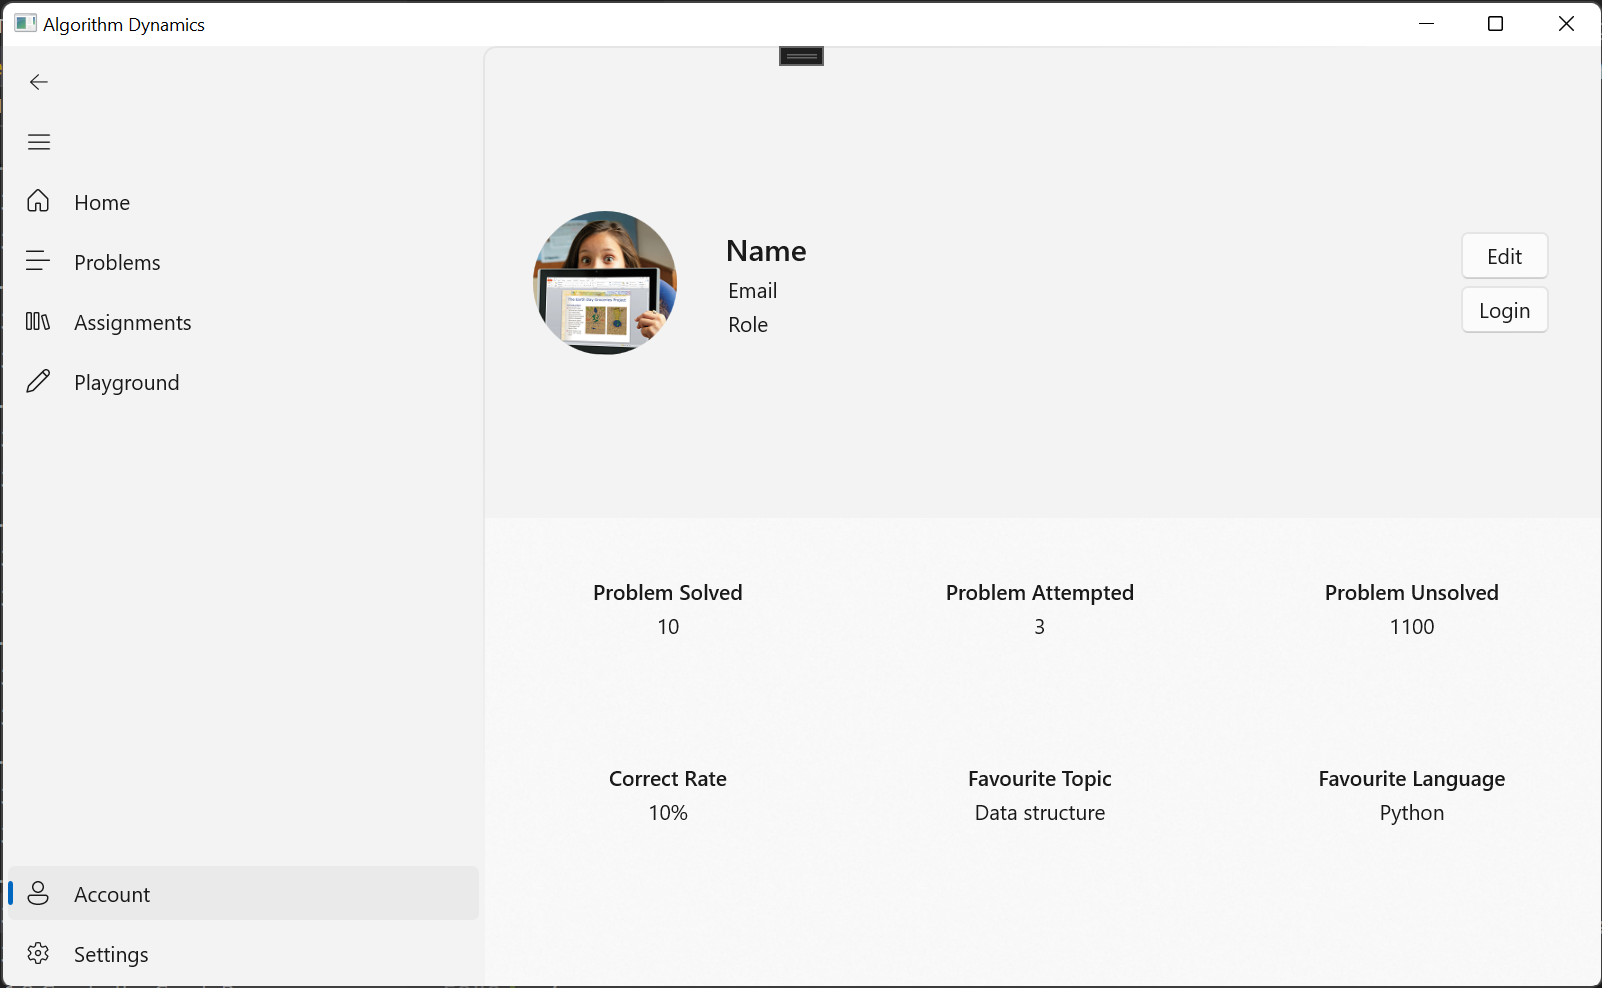
\includegraphics[width=\textwidth, height=\textheight, keepaspectratio]{AccountPage-Layout}

Next, I want to implement the edit function, which allows the user to change their user name, email address and role. To achieve this, I decide to replace the TextBlocks with TextBoxes for the user to edit the data when the Edit button is clicked. This can be achieved by setting the visibility of the controls. Instead of directly setting the visibility, I decide to bind the visibility property to a public variable named \code{IsEditMode} to determine whether it should display. In order to notify the binded control, I implement the \code{PropertyChanged} event\cite{microsoft:docs:data-binding-in-depth}.

\begin{minted}{csharp}
/// <summary>
/// Invoke when the property is changed.
/// </summary>
public event PropertyChangedEventHandler PropertyChanged = delegate { };

/// <summary>
/// Invoke a new <see cref="PropertyChanged"/> event.
/// </summary>
/// <param name="propertyName">Use <see cref="nameof"/> to get the name of the property.</param>
public void OnPropertyChanged([CallerMemberName] string propertyName = null)
{
    // Raise the PropertyChanged event, passing the name of the property whose value has changed.
    PropertyChanged?.Invoke(this, new PropertyChangedEventArgs(propertyName));
}
\end{minted}

I create a private variable \code{_isEditMode} to record the current state. A public variable \code{IsEditMode} to encapsulated the private variable so I can call the \code{OnPropertyChanged} function I just implemented in the setter. I also create the \code{IsNotEditMode} attribute to handle the boolean inversion.

\begin{minted}{csharp}
private bool _isEditMode = false;
public bool IsEditMode
{
    get => _isEditMode;
    set
    {
        _isEditMode = value;
        OnPropertyChanged(nameof(IsEditMode));
        OnPropertyChanged(nameof(IsNotEditMode));
    }
}
public bool IsNotEditMode
{
    get => !_isEditMode;
}
\end{minted}

Finally, I edit the XAML markup to add the TextBoxes and add the bindings.


\begin{minted}{xml}
<StackPanel
    RelativePanel.RightOf="AvatarPicture"
    RelativePanel.AlignVerticalCenterWithPanel="True">
    <TextBlock
        x:Name="NameTextBlock"
        Margin="2"
        Text="{x:Bind EditNameTextBox.Text, Mode=OneWay}"
        Visibility="{x:Bind IsNotEditMode, Mode=OneWay"
        Style="{ThemeResource SubtitleTextBlockStyle}"/>
    <TextBox
        x:Name="EditNameTextBox"
        PlaceholderText="Name"
        Margin="2"
        Text="Name"
        HorizontalAlignment="Stretch"
        Visibility="{x:Bind IsEditMode, Mode=OneWay"/>
    <TextBlock
        x:Name="EmailTextBlock"
        Margin="2"
        Text="{x:Bind EditEmailTextBox.Text, Mode=OneWay}"
        Visibility="{x:Bind IsNotEditMode, Mode=OneWay"
        Style="{ThemeResource BodyTextBlockStyle}"/>
    <TextBox
        x:Name="EditEmailTextBox"
        PlaceholderText="Email"
        Text="Email"
        Margin="2"
        HorizontalAlignment="Stretch"
        Visibility="{x:Bind IsEditMode, Mode=OneWay"/>
    <TextBlock
        x:Name="RoleTextBlock"
        Margin="2"
        Text="{x:Bind EditRoleComboBox.SelectedValue, Mode=OneWay}"
        Visibility="{x:Bind IsNotEditMode, Mode=OneWay"
        Style="{ThemeResource BodyTextBlockStyle}"/>
    <ComboBox
        x:Name="EditRoleComboBox"
        Visibility="{x:Bind IsEditMode, Mode=OneWay"
        HorizontalAlignment="Stretch"
        Margin="2"
        SelectedIndex="0">
        <x:String>Student</x:String>
        <x:String>Teacher</x:String>
    </ComboBox>
</StackPanel>
\end{minted}

Now when I run the program, I can edit all fields successfully after clicking the Edit button. All the changes are preserved after clicking the Done button.

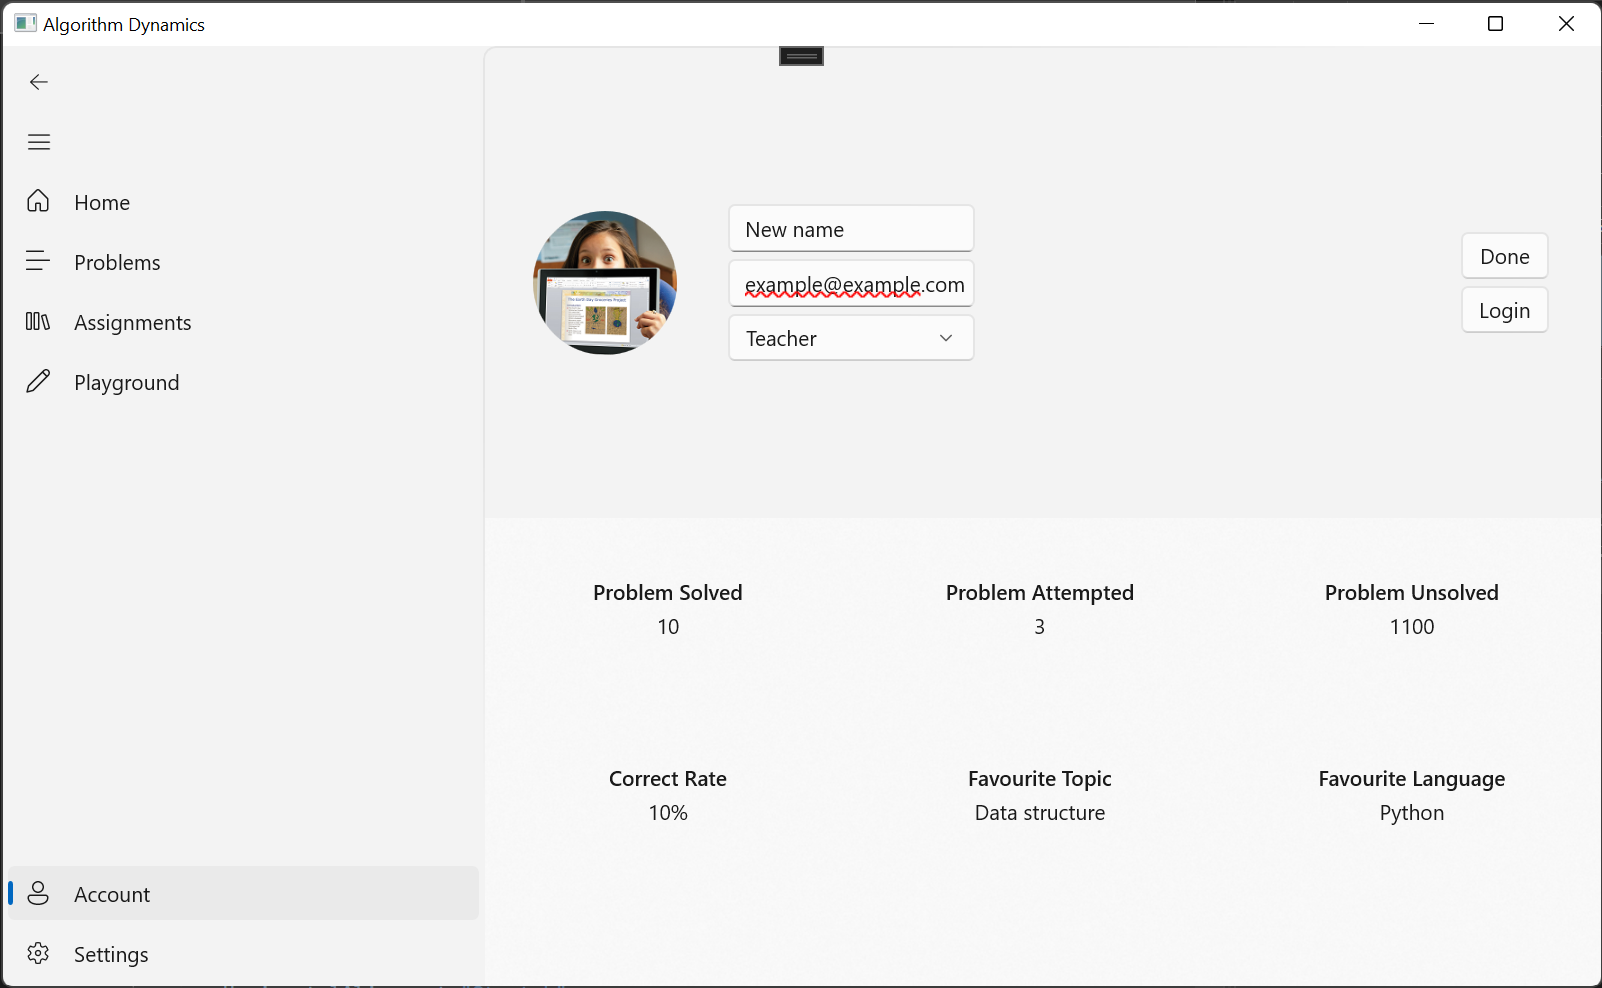
\includegraphics[width=\textwidth, height=\textheight, keepaspectratio]{AccountPage-Edit}

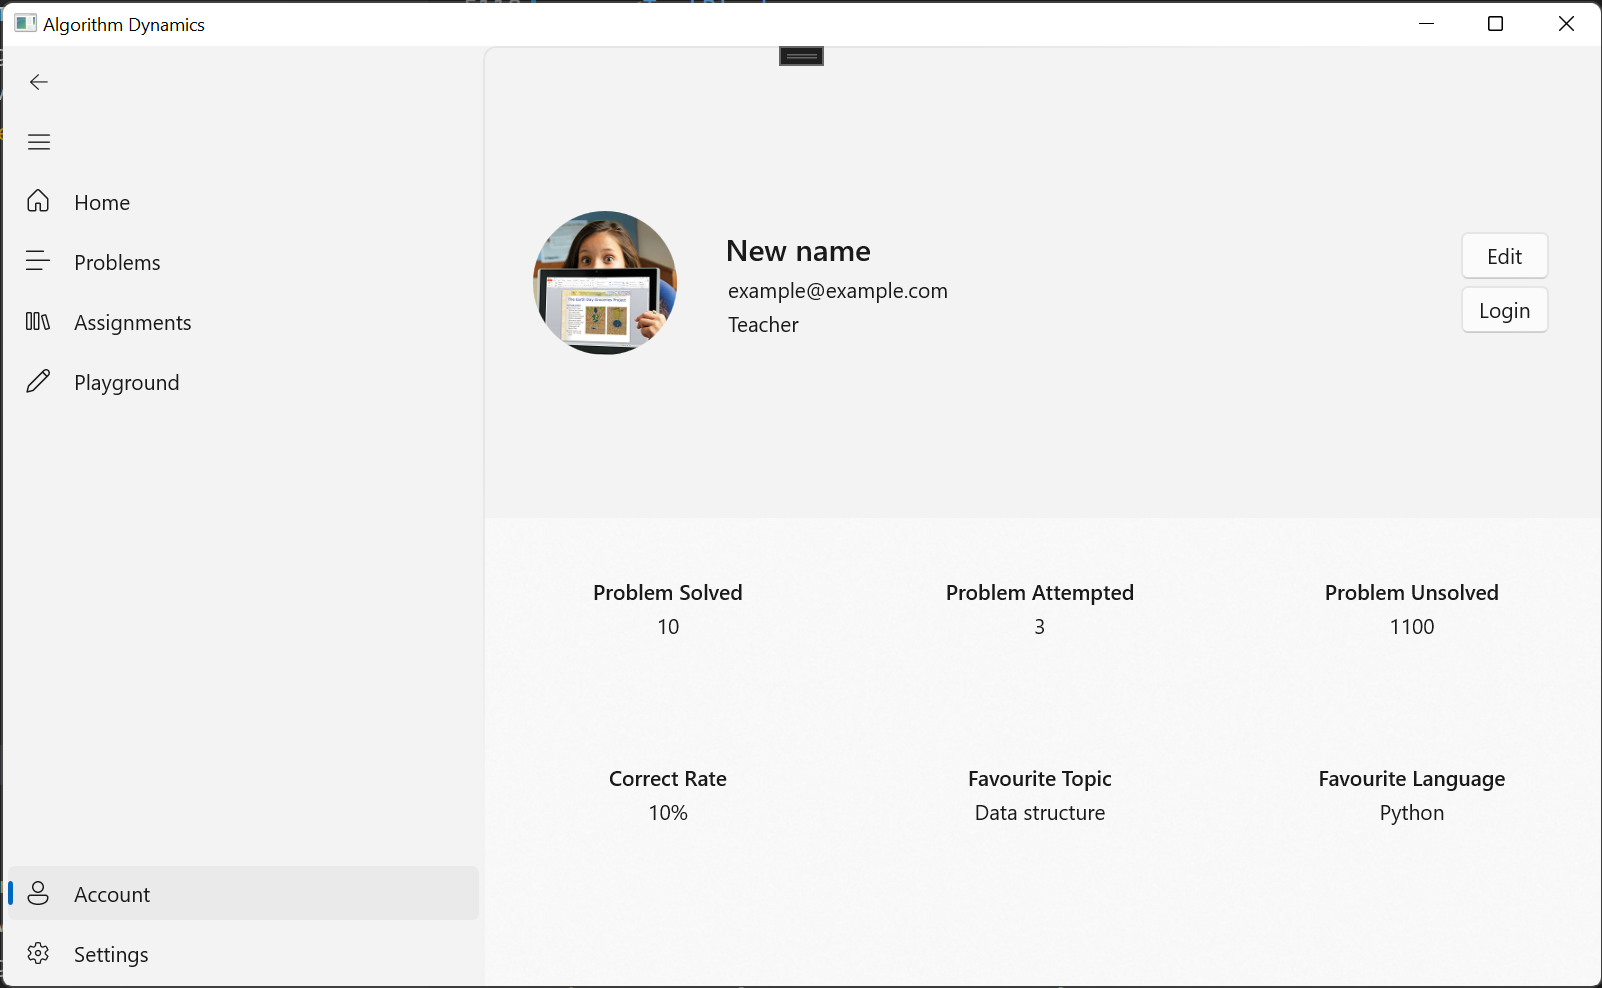
\includegraphics[width=\textwidth, height=\textheight, keepaspectratio]{AccountPage-Saved}

\subsubsection{Testing and validation}

\begin{tabulary}{\linewidth}{|L|l|L|}
    \hline
    Test & Result & Remark \\
    \hline
    Does it load & Pass & \\
    \hline
    Does the Edit button work & Pass & Note that the changes are not actually saved to the disk, since the settings module will not be implemented in this iteration. \\
    \hline
    Does the login button work & Failed & The login button depends on the API module, which will not be implemented in this iteration. \\
    \hline
    Does the statistics data show up correctly & Pass & Note that the actual data depends on the database module, which is not implemented yet. \\
    \hline
\end{tabulary}

\subsection{Create the CreatePage}

\subsubsection{Implementation}

For the CreateNewProblemPage, it contains a form for the user to input data to create new problems. I use a ScrollViewer to wrap everything up so the user can scroll in the page when the elements overflow. Inside the ScrollViewer, I place a StackPanel as the root panel to organize everything.

\begin{minted}{xml}
<ScrollViewer x:Name="scrollViewer">
    <StackPanel
        Margin="32"
        x:Name="FormStackPanel">
        <!-- Form controls -->
    </StackPanel>
</ScrollViewer>
\end{minted}

I use TextBoxes to allow the user to input problem name, a TokenizingTextBox for the tag, ComboBox for difficult, and NumberBox for time limit and memory limit.

\begin{minted}{xml}
<TextBlock
    Text="Create Problem"
    Style="{ThemeResource TitleTextBlockStyle}"/>
<TextBox
    Margin="0 22 0 0"
    Header="Problem Name"
    MaxLength="64"
    Width="400"
    HorizontalAlignment="Left"/>
<controls:TokenizingTextBox
    Header="Tags"
    Margin="0 22 0 0" 
    Width="400"
    MaximumTokens="3"
    PlaceholderText="Add Tags"
    SelectionMode="Extended"
    HorizontalAlignment="Left"/>
<ComboBox
    Header="Difficulty"
    SelectedIndex="0"
    Margin="0 22 0 0"
    Width="400"
    HorizontalAlignment="Left">
    <x:String>Easy</x:String>
    <x:String>Medium</x:String>
    <x:String>Hard</x:String>
</ComboBox>
<NumberBox
    Header="Time Limit (ms)"
    Value="1000"
    Width="400"
    Minimum="100"
    Margin="0 22 0 0"
    HorizontalAlignment="Left"
    SpinButtonPlacementMode="Inline"
    SmallChange="100"
    LargeChange="500"/>
<NumberBox
    Header="Memory Limit (MB)"
    Value="64"
    Width="400"
    Margin="0 22 0 0"
    Minimum="16"
    HorizontalAlignment="Left"
    SpinButtonPlacementMode="Inline"
    SmallChange="64"
    LargeChange="256"/>
\end{minted}

For the description, I use a Pivot to organize the input TextBox and the preview MarkdownRenderer.

\begin{minted}{xml}
<Pivot
    x:Name="DescriptionPivot">
    <PivotItem
        Header="Description">
        <TextBox
            x:Name="DescriptionTextBox"
            HorizontalAlignment="Stretch"
            VerticalAlignment="Stretch"
            TextWrapping="Wrap" 
            AcceptsReturn="True" 
            IsSpellCheckEnabled="True"
            MinHeight="200"
            MaxHeight="840"/>
    </PivotItem>
    <PivotItem
        Header="Preview">
        <controls:MarkdownTextBlock
            x:Name="ProblemMarkdownTextBlock"
            Margin="8"
            Background="{ThemeResource ApplicationPageBackgroundThemeBrush}"
            Text="{x:Bind DescriptionTextBox.Text, Mode=OneWay}"/>
    </PivotItem>
</Pivot>
\end{minted}

Next, I implement the TestCase list. Similarly as the ProblemList before, I use a ListView and bind the TestCases collection to it.

\begin{minted}{xml}
<ListView
    x:Name="TestCasesListView"
    Margin="0 22 0 0"
    Header="Test Cases"
    SelectionMode="None"
    ItemsSource="{x:Bind TestCases, Mode=OneWay}">
    <ListView.ItemTemplate>
        <DataTemplate x:DataType="local:TestCase">
            <Grid
                Margin="0 10 0 0">
                <Grid.ColumnDefinitions>
                    <ColumnDefinition Width="*"/>
                    <ColumnDefinition Width="*"/>
                    <ColumnDefinition Width="auto"/>
                    <ColumnDefinition Width="auto"/>
                </Grid.ColumnDefinitions>
                <TextBox
                    Grid.Column="0"
                    Margin="4"
                    AcceptsReturn="True"
                    MaxHeight="100"
                    VerticalAlignment="Center"
                    PlaceholderText="Input Data"
                    Text="{x:Bind Input, Mode=TwoWay}"/>
                <TextBox
                    Grid.Column="1"
                    Margin="4"
                    AcceptsReturn="True"
                    MaxHeight="100"
                    VerticalAlignment="Center"
                    PlaceholderText="Output Data"
                    Text="{x:Bind Output, Mode=TwoWay}"/>
                <CheckBox
                    Grid.Column="2"
                    Margin="40 0 0 0"
                    Content="Example"
                    HorizontalAlignment="Center"
                    VerticalAlignment="Center"
                    IsChecked="{x:Bind IsExample, Mode=TwoWay}"/>
                <Button
                    x:Name="DeleteSingleTestCaseButton"
                    Grid.Column="3"
                    Margin="0"
                    VerticalAlignment="Center"
                    HorizontalAlignment="Center"
                    Click="DeleteSingleTestCase">
                    <Button.Content>
                        <SymbolIcon Symbol="Delete"/>
                    </Button.Content>
                </Button>
            </Grid>
        </DataTemplate>
    </ListView.ItemTemplate>
</ListView>
\end{minted}

\begin{minted}{csharp}
public ObservableCollection<TestCase> TestCases = new() { new TestCase("", "", true) };
\end{minted}


I implement a simple TestCase class for this iteration, so the UI can be tested. A more detailed one will be implemented in the later iteration.

\begin{minted}{csharp}
public class TestCase
{
    public string Input { get; set; }
    public string Output { get; set; }
    public bool IsExample { get; set; }
    public TestCase(string input, string output, bool isExample)
    {
        Input = input;
        Output = output;
        IsExample = isExample;
    }
}
\end{minted}

I add another StackPanel to organize the buttons to add new test cases and delete all test cases.

\begin{minted}{xml}
<StackPanel 
    Margin="0 12 0 0"
    HorizontalAlignment="Right"
    Orientation="Horizontal">
    <Button
        x:Name="AddTestCaseButton"
        Click="AddTestCase">
        <Button.Content>
            <SymbolIcon Symbol="Add"/>
        </Button.Content>
    </Button>
    <Button 
        Margin="4 0 12 0">
        <Button.Content>
            <SymbolIcon Symbol="Delete"/>
        </Button.Content>
        <Button.Flyout>
            <Flyout x:Name="DeleteConfirmFlyout">
                <StackPanel>
                    <TextBlock Style="{ThemeResource BaseTextBlockStyle}" Text="All test cases will be deleted. Do you want to continue?" Margin="0,0,0,12" />
                    <Button HorizontalAlignment="Right" Click="DeleteAllTestCases"  Content="Yes" />
                </StackPanel>
            </Flyout>
        </Button.Flyout>
    </Button>
</StackPanel>
\end{minted}

At the bottom of the page, a StackPanel is used to organize the save and cancel button. Flyouts are added to all delete and cancel buttons to confirm before actually performing the action.

\begin{minted}{xml}
<StackPanel 
    Margin="0 12 12 0"
    HorizontalAlignment="Left"
    Orientation="Horizontal">
    <Button 
        Margin="0 0 4 0"
        Content="Save"
        Width="100"
        Click="CreateProblem"
        Style="{ThemeResource AccentButtonStyle}"/>
    <Button 
        Width="100"
        Content="Cancel">
        <Button.Flyout>
            <Flyout x:Name="CancelConfirmFlyout">
                <StackPanel>
                    <TextBlock
                        Style="{ThemeResource BaseTextBlockStyle}"
                        Text="All changes will be lost. Do you want to continue?" Margin="0 0 0 12" />
                    <Button 
                        HorizontalAlignment="Right" 
                        Click="CancelCreation"  
                        Content="Yes" />
                </StackPanel>
            </Flyout>
        </Button.Flyout>
    </Button>
</StackPanel>
</StackPanel>
\end{minted}

The CreateNewProblemPage can be navigated to from the ProblemsPage. I connect the add problem in the ProblemsPage to the navigation function. Instead of manually navigate through the ContentFrame, I decide to encapsulate the management of the NavigationView through an App.NavigateTo function. Which enables me to reuse this part of code, and make it less likely for me to get the navigation wrong in the future. I expose the \code{m_window} and the \code{MainNavView} as global static variables, so the can be accessed easily in the App level.

\begin{minted}{csharp}
public static MainWindow m_window;
public static NavigationView MainNavView { get => m_window.MainNavView; }
public static Frame ContentFrame { get => m_window.ContentFrame; }

\end{minted}

\begin{minted}{csharp}
/// <summary>
/// Navigate to the <see cref="CreateNewProblemPage"/> to create a new <see cref="Problem"/>.
/// </summary>
/// <param name="sender"></param>
/// <param name="e"></param>
private void CreateNewProblem(object sender, RoutedEventArgs e)
{
    App.NavigateTo(typeof(CreateNewProblemPage));
}
/// <summary>
/// Handle the navigation of the main <see cref="ContentFrame"/>
/// When the page is listed in the <see cref="MainNavView"/>, 
/// change the <see cref="MainNavView.SelectedItem"/> directly.
/// Otherwise, set the <see cref="MainNavView.SelectedItem"/> to null and 
/// apply the navigation on the Frame directly.
/// </summary>
/// <param name="type"></param>
/// <param name="parameter"></param>
public static void NavigateTo(Type type, object parameter = null)
{
    if (type == typeof(HomePage))
        MainNavView.SelectedItem = MainNavView.MenuItems[0];
    else if (type == typeof(ProblemsPage))
        MainNavView.SelectedItem = MainNavView.MenuItems[1];
    else if (type == typeof(AssignmentsPage))
        MainNavView.SelectedItem = MainNavView.MenuItems[2];
    else if (type == typeof(PlaygroundPage))
        MainNavView.SelectedItem = MainNavView.MenuItems[3];
    else if (type == typeof(AccountPage))
        MainNavView.SelectedItem = MainNavView.FooterMenuItems[0];
    else if (type == typeof(SettingsPage))
        MainNavView.SelectedItem = MainNavView.SettingsItem;
    else
    {
        ContentFrame.Navigate(type, parameter);
        MainNavView.SelectedItem = null;
    }
}
\end{minted}

Now I can easily navigate to the CreateNewProblemPage with the \code{NavigateTo} function.

\begin{minted}{csharp}
/// <summary>
/// Navigate to the <see cref="CreateNewProblemPage"/> to create a new <see cref="Problem"/>.
/// </summary>
/// <param name="sender"></param>
/// <param name="e"></param>
private void CreateNewProblem(object sender, RoutedEventArgs e)
{
    App.NavigateTo(typeof(CreateNewProblemPage));
}
\end{minted}

When I click the Add Problem button in the ProblemsPage, the ContentFrame navigates to the CreateNew Page successfully. The MainNavView is deselected correctly as well.

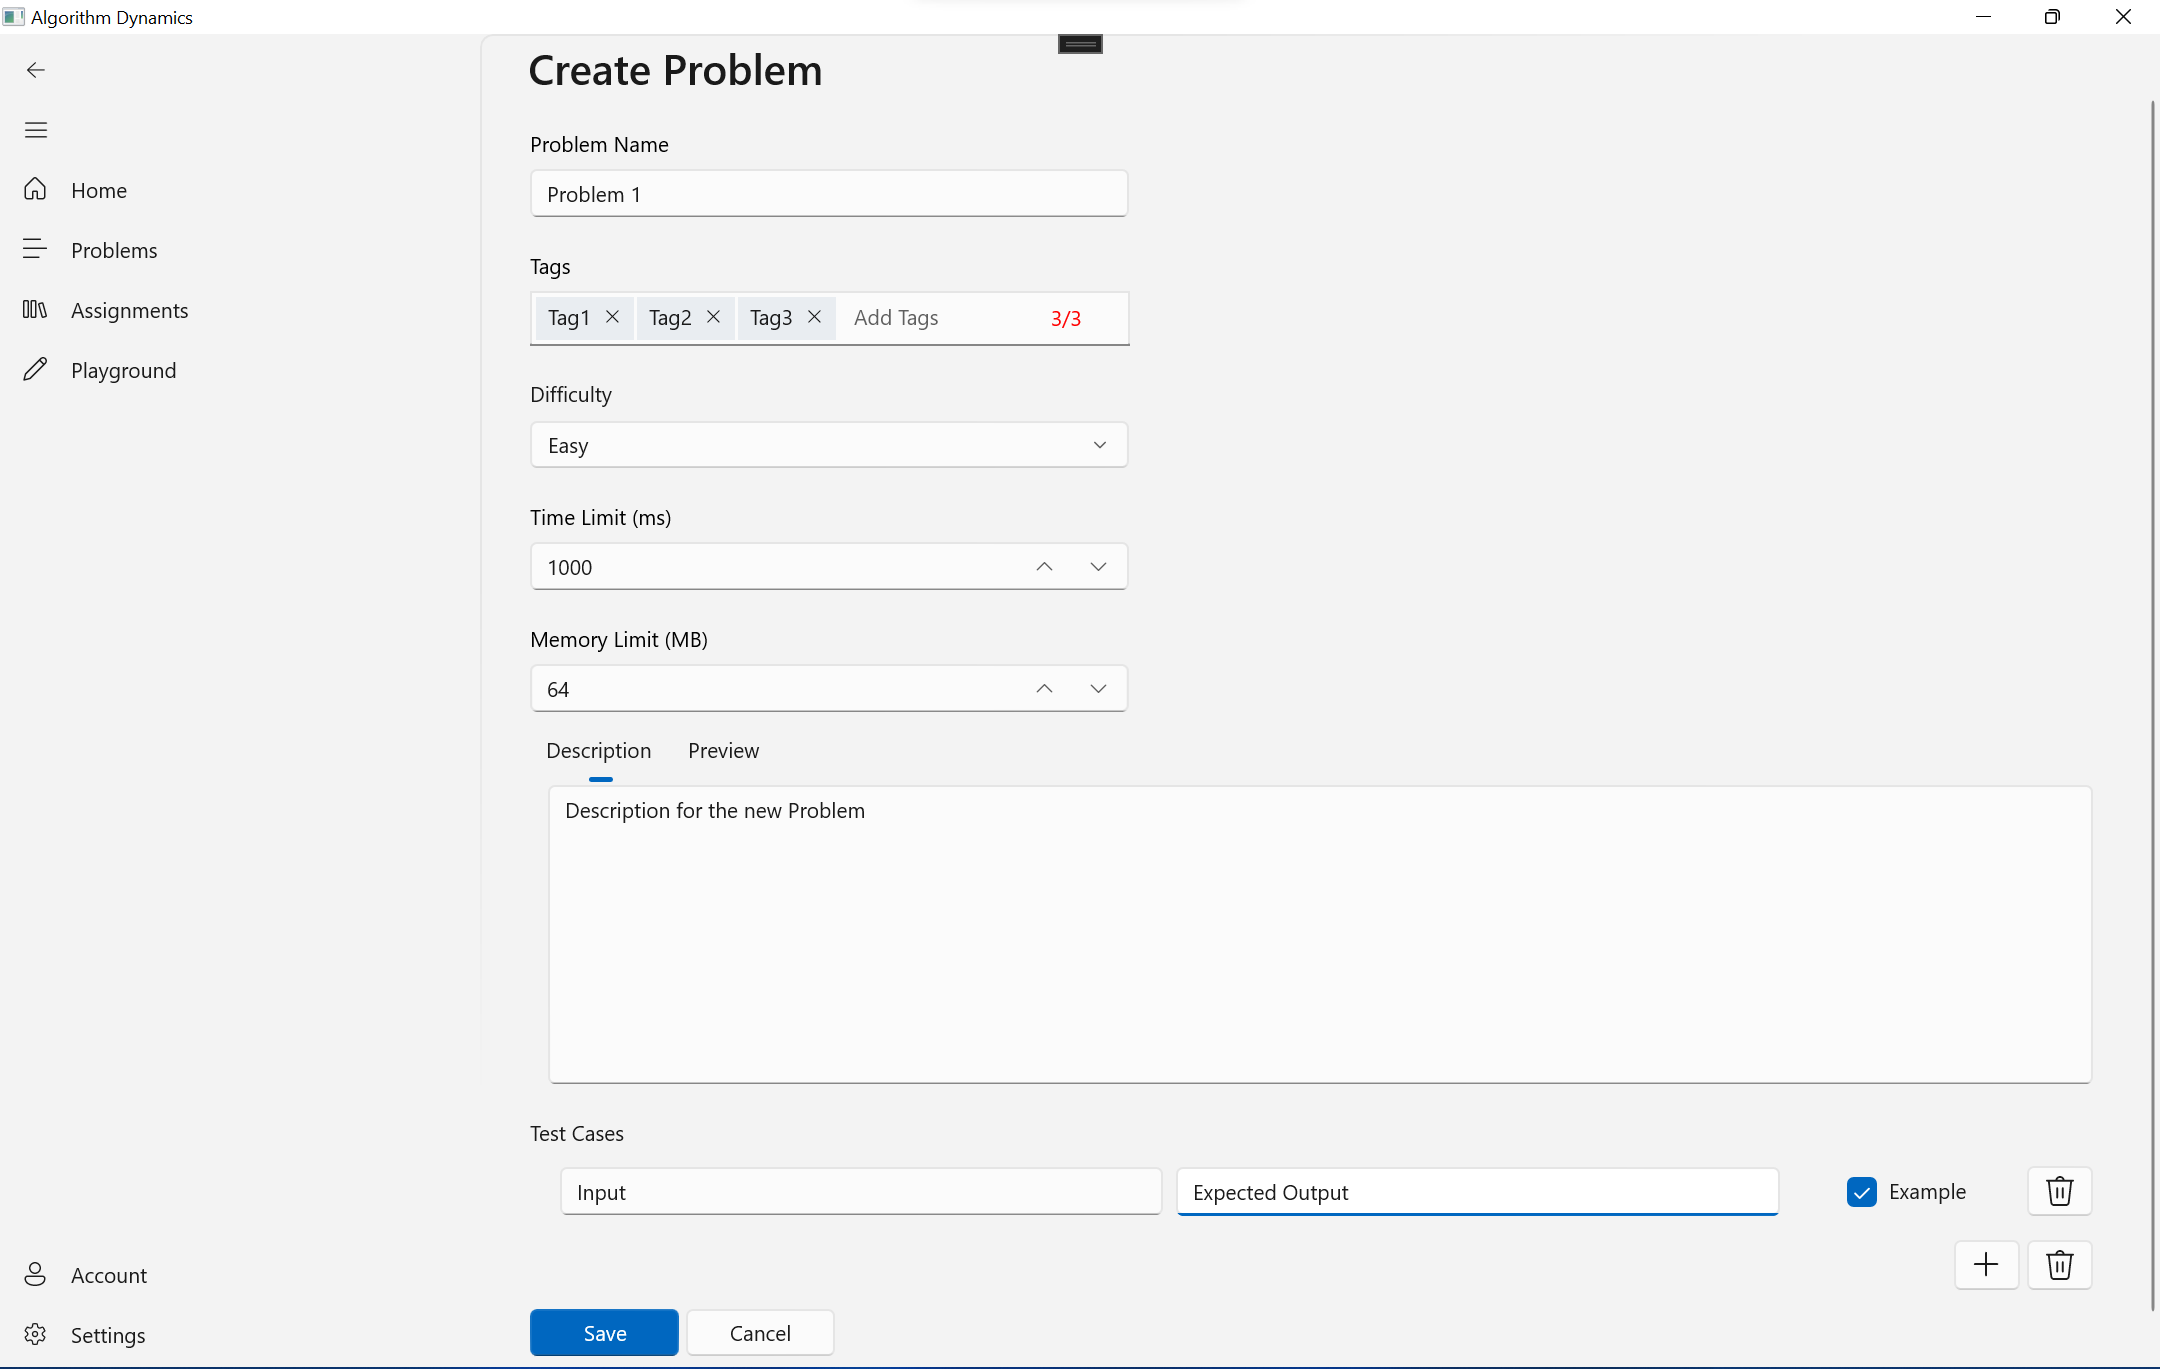
\includegraphics[width=\textwidth, height=\textheight, keepaspectratio]{CreateNewProblemPage-Layout}

I can input all data for a new problem. The length validation for the problem name and the tag box is working as intended. The time limit field and memory limit field also rejecte any non-numerical input as intended. However, when I try to delete a token in the TokenizingTextBox, an exception is thrown and the app crashes.

\begin{minted}{text}
Unhandled exception at 0x00007FFCDA3E6328 (Microsoft.ui.xaml.dll) in Algorithm Dynamics.exe: 0xC000027B: An application-internal exception has occurred (parameters: 0x000001DCA9C47860, 0x0000000000000006).
\end{minted}

It seems to be an internal issue with Microsoft.ui.xaml.dll. After some research, I found that this is caused by an internal bug with the TokenizingTextBox\cite{github:WindowsCommunityToolkit:4437}. I will keep an eye on the issue and update the dependency as soon as it gets fixed. For now, I will just leave it as this and mark this as a known issue.

Next, I implement a series of functions in the code behind to handle the add delete test case function, and the save cancel function.

\begin{minted}{csharp}
/// <summary>
/// Add a new <see cref="TestCase"/> to the list.
/// Scroll the <see cref="scrollViewer"/> to the new position.
/// </summary>
/// <param name="sender"></param>
/// <param name="e"></param>
private void AddTestCase(object sender, RoutedEventArgs e)
{
    TestCases.Add(new TestCase("", "", false));
    GeneralTransform transform = AddTestCaseButton.TransformToVisual((UIElement)scrollViewer.Content);
    Point position = transform.TransformPoint(new Point(0, 0));
    scrollViewer.ChangeView(null, position.Y, null, false);
}

/// <summary>
/// Delete the selected <see cref="TestCase"/>. Update the <see cref="TestCase.Id"/>.
/// </summary>
/// <param name="sender"></param>
/// <param name="e"></param>
private void DeleteSingleTestCase(object sender, RoutedEventArgs e)
{
    TestCase selectedItem = ((FrameworkElement)sender).DataContext as TestCase;
    TestCases.Remove(selectedItem);
}

/// <summary>
/// Delete all <see cref="TestCase"/>, hide the <see cref="DeleteConfirmFlyout"/>.
/// </summary>
/// <param name="sender"></param>
/// <param name="e"></param>
private void DeleteAllTestCases(object sender, RoutedEventArgs e)
{
    TestCases.Clear();
    DeleteConfirmFlyout.Hide();
}

/// <summary>
/// Cancel the creation, navigate back to the <see cref="ProblemsPage"/>.
/// </summary>
/// <param name="sender"></param>
/// <param name="e"></param>
private void CancelCreation(object sender, RoutedEventArgs e)
{
    CancelConfirmFlyout.Hide();
    App.NavigateTo(typeof(ProblemsPage));
}

/// <summary>
/// Create the problem and save it into the database.
/// Navigate back to the <see cref="ProblemsPage"/> afterwards.
/// </summary>
/// <param name="sender"></param>
/// <param name="e"></param>
private void CreateProblem(object sender, RoutedEventArgs e)
{
    // TODO save the Problem to database
    App.NavigateTo(typeof(ProblemsPage));
}
\end{minted}

For the edit problem page, I find that there is not much difference from the create page. The edit problem page is just a create problem page with a different title, and some pre-loaded problem data. I think I can reuse most of the existing code to implement the edit page.

I add an enumeration of \code{Mode} to the page to specify whether it is a create page or an edit page.

\begin{minted}{csharp}
public enum Mode
{
    Create,
    Edit
}
private Mode PageMode = Mode.Create;
\end{minted}

I use a private readonly variable \code{_title} to store the string of the title of the page. It determines the correct title for the page based on the page mode.

\begin{minted}{csharp}
private string _title
{
    get
    {
        if (PageMode == Mode.Create)
            return "Create Problem";
        else
            return "Edit Problem";
    }
}
\end{minted}

I bind the title TextBox to the \code{_title} variable. Each time when the page is loaded, its value is recalculated and the correct one will be displayed.

\begin{minted}{xml}
<TextBlock
    Text="{x:Bind _title, Mode=OneTime}"
    Style="{ThemeResource TitleTextBlockStyle}"/>
\end{minted}

To allow the page mode to be set, I need to handle the OnNavigatedTo event and process the arguments correctly to retrieve the page mode.

\begin{minted}{csharp}
/// <summary>
/// Handle the Navigation Arguments
/// Set the <see cref="PageMode"/> if the Parameter is not <see cref="null"/>.
/// </summary>
/// <param name="e"></param>
protected override void OnNavigatedTo(NavigationEventArgs e)
{
    if (e.Parameter != null)
    {
        PageMode = ((Tuple<Mode, int>)e.Parameter).Item1;
    }
    base.OnNavigatedTo(e);
}
\end{minted}

Now, I can connect the edit button in the ProblemsPage to the edit page mode, so the correct title is displayed.

\begin{minted}{csharp}
private Problem _problem;
/// <summary>
/// Handle the Navigation Arguments
/// Set the <see cref="_pageMode"/> if the Parameter is not <see cref="null"/>.
/// </summary>
/// <param name="e"></param>
protected override void OnNavigatedTo(NavigationEventArgs e)
{
    if (e.Parameter != null)
    {
        var parameter = (Tuple<Mode, Problem>)e.Parameter;
        _pageMode = parameter.Item1;
        _problem = parameter.Item2;
    }
    base.OnNavigatedTo(e);
}
\end{minted}

Now when I right click a problem in the ProblemsPage and click the edit button in the flyout, the edit page mode is loaded correctly with the problem data being filled for me.

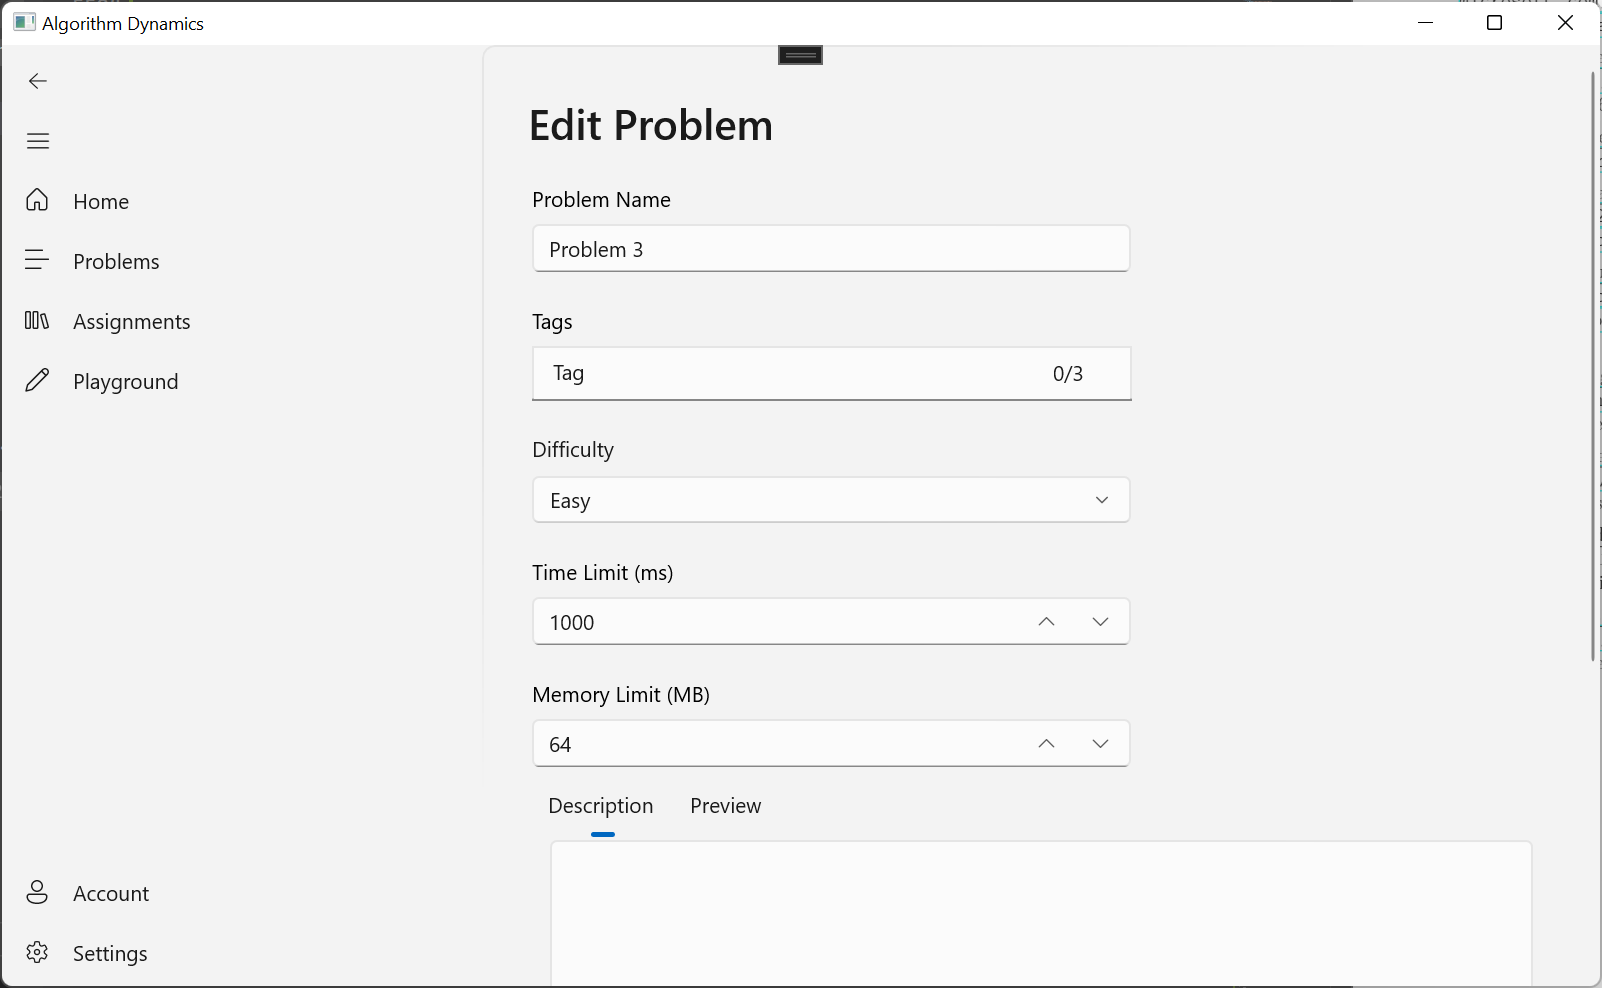
\includegraphics[width=\textwidth, height=\textheight, keepaspectratio]{CreateNewProblemPage-Edit}

For the CreateNewProblemListPage, I create it in a very similar way - but with different fields and options.

\begin{minted}{xml}
<ScrollViewer x:Name="scrollViewer">
    <StackPanel
        Margin="32"
        x:Name="FormStackPanel">
        <TextBlock
            Text="{x:Bind _title, Mode=OneTime}"
            Style="{ThemeResource TitleTextBlockStyle}"/>
        <TextBox
            Margin="0 22 0 0"
            Header="Title"
            MaxLength="64"
            Width="400"
            HorizontalAlignment="Left"/>
        <CalendarDatePicker 
            Margin="0 22 0 0"
            Visibility="{x:Bind _isAssignmentMode, Mode=OneTime}"
            PlaceholderText="Set the due date" 
            Header="Due Date"/>
        <TextBox
            Margin="0 22 0 0"
            Header="Description"
            HorizontalAlignment="Left"
            TextWrapping="Wrap" 
            AcceptsReturn="True" 
            IsSpellCheckEnabled="True"
            MinWidth="400"
            MinHeight="200"
            MaxHeight="840"/>
        <AutoSuggestBox
            x:Name="AddProblemBox"
            Header="Add Problems"
            Margin="0 22 0 0"
            HorizontalAlignment="Left"
            QueryIcon="Find"
            Width="400"
            TextChanged="AddProblemBox_TextChanged"
            SuggestionChosen="AddProblemBox_SuggestionChosen"/>
        <ListView
            Margin="0 22 0 0"
            SelectionMode="None"
            ItemsSource="{x:Bind Problems, Mode=OneWay}">
            <ListView.ItemTemplate>
                <DataTemplate x:DataType="local:Problem">
                    <Grid
                        Margin="0 10 0 0">
                        <Grid.ColumnDefinitions>
                            <ColumnDefinition Width="*"/>
                            <ColumnDefinition Width="*"/>
                            <ColumnDefinition Width="*"/>
                            <ColumnDefinition Width="*"/>
                        </Grid.ColumnDefinitions>
                        <TextBlock
                            Grid.Column="0"
                            VerticalAlignment="Center"
                            Text="{x:Bind Name}"/>
                        <TextBlock
                            Grid.Column="1"
                            VerticalAlignment="Center"
                            Text="{x:Bind Difficulty}"/>
                        <TextBlock
                            Grid.Column="2"
                            VerticalAlignment="Center"
                            Text="{x:Bind Tags}"/>
                        <Button
                            x:Name="DeleteButton"
                            Grid.Column="3"
                            HorizontalAlignment="Right"
                            Click="DeleteSingleTestCase">
                            <Button.Content>
                                <SymbolIcon Symbol="Delete"/>
                            </Button.Content>
                        </Button>
                    </Grid>
                </DataTemplate>
            </ListView.ItemTemplate>
        </ListView>
        <StackPanel 
            Margin="0 22 12 0"
            HorizontalAlignment="Left"
            Orientation="Horizontal">
            <Button
                x:Name="SaveButton"
                Content="Save"
                Width="100"
                Margin="0 0 4 0"
                Click="SaveButton_Click"
                Style="{ThemeResource AccentButtonStyle}">
                <Button.Flyout>
                    <Flyout
                        x:Name="SaveFlyout">
                        <StackPanel>
                            <TextBlock 
                                x:Name="TestTextBlock"
                                Style="{ThemeResource BaseTextBlockStyle}"
                                Text="The Problem List is not saved." 
                                Margin="0 0 0 12" />
                            <StackPanel 
                                Orientation="Horizontal"
                                HorizontalAlignment="Right">
                                <Button
                                    x:Name="DoneButton"
                                    Margin="0 0 4 0"
                                    Content="Done"
                                    Click="Finish"/>
                                <Button 
                                    x:Name="ExportButton"
                                    Click="ExportAndFinish"
                                    Style="{ThemeResource AccentButtonStyle}"
                                    Content="Export"/>
                            </StackPanel>
                        </StackPanel>
                    </Flyout>
                </Button.Flyout>
            </Button>
            <Button
                Content="Cancel"
                Width="100">
                <Button.Flyout>
                    <Flyout>
                        <StackPanel>
                            <TextBlock
                                Style="{ThemeResource BaseTextBlockStyle}"
                                Text="All changes will be lost. Do you want to continue?" Margin="0 0 0 12" />
                            <Button 
                                HorizontalAlignment="Right" 
                                Click="Finish"
                                Content="Yes" />
                        </StackPanel>
                    </Flyout>
                </Button.Flyout>
            </Button>
        </StackPanel>
    </StackPanel>
</ScrollViewer>
\end{minted}

Similarly, I reuse the same page for create/edit ProblemList and Assignments by managing different page mode.

\begin{minted}{csharp}
public enum Mode
{
    CreateProblemList,
    EditProblemList,
    CreateAssignment,
    EditAssignment
}
private Mode _pageMode = Mode.CreateProblemList;
private bool _isAssignmentMode { get => _pageMode == Mode.CreateAssignment || _pageMode == Mode.EditAssignment; }
private string _title
{
    get
    {
        if (_pageMode == Mode.CreateProblemList)
            return "Create Problem List";
        else if (_pageMode == Mode.EditProblemList)
            return "Edit Problem List";
        else if (_pageMode == Mode.CreateAssignment)
            return "Create Assignment";
        else
            return "Edit Assignment";
    }
}

/// <summary>
/// Handle the Navigation Arguments
/// Set the <see cref="_pageMode"/> if the Parameter is not <see cref="null"/>.
/// </summary>
/// <param name="e"></param>
protected override void OnNavigatedTo(NavigationEventArgs e)
{
    if (e.Parameter != null)
    {
        _pageMode = ((Tuple<Mode>)e.Parameter).Item1;
    }
    base.OnNavigatedTo(e);
}
\end{minted}


Differently, instead of asking the user to create new test cases, the user is required to search and select problems from the existing database. I use a procedure to handle the event when the user is inputing in the search box.

\begin{minted}{csharp}
/// <summary>
/// When the text is changed in the search box, search in the database and create suggestion items. 
/// </summary>
/// <param name="sender"></param>
/// <param name="args"></param>
private void AddProblemBox_TextChanged(AutoSuggestBox sender, AutoSuggestBoxTextChangedEventArgs args)
{
    if (args.Reason == AutoSuggestionBoxTextChangeReason.UserInput)
    {
        var suitableItems = new List<string>();
        suitableItems.Add(sender.Text);
        // TODO search the actual problem from the database
        if (suitableItems.Count == 0)
        {
            suitableItems.Add("No results found");
        }
        sender.ItemsSource = suitableItems;
    }

}
/// <summary>
/// When a suggestion is chosen, add it in to the list.
/// </summary>
/// <param name="sender"></param>
/// <param name="args"></param>
private void AddProblemBox_SuggestionChosen(AutoSuggestBox sender, AutoSuggestBoxSuggestionChosenEventArgs args)
{
    Problems.Add(new Problem(sender.Text, "Easy", "ToDo", "Data structure"));
}
\end{minted}

When the user clicks the delete button on a problem, I use a procedure to delete the problem from the list.

\begin{minted}{csharp}
/// <summary>
/// Delete the selected problem from the list.
/// </summary>
/// <param name="sender"></param>
/// <param name="e"></param>
private void DeleteSingleProblem(object sender, RoutedEventArgs e)
{
    Problem selectedItem = ((FrameworkElement)sender).DataContext as Problem;
    Problems.Remove(selectedItem);
}
\end{minted}

When the user click the save button, I use a procedure to save the problem to the database.

\begin{minted}{csharp}
/// <summary>
/// When the save button is clicked, save the problem list and change the description test.
/// </summary>
/// <param name="sender"></param>
/// <param name="e"></param>
private void SaveButton_Click(object sender, RoutedEventArgs e)
{
    // TODO actually save the problem to the database.
    TestTextBlock.Text = "The Problem List is saved.";
}
\end{minted}

When the user has finished editing, a procedure will hide all the flyouts and navigate the user back to the ProblemsPage.

\begin{minted}{csharp}
/// <summary>
/// Finish create or edit the ProblemList or Assignment.
/// Go back to <see cref="ProblemsPage"/> or <see cref="AssignmentsPage"/> based on <see cref="_pageMode"/>.
/// </summary>
/// <param name="sender"></param>
/// <param name="e"></param>
private void Finish(object sender, RoutedEventArgs e)
{
    SaveFlyout.Hide();
    if (_pageMode == Mode.CreateProblemList || _pageMode == Mode.EditProblemList)
        App.NavigateTo(typeof(ProblemsPage));
    else
        App.NavigateTo(typeof(AssignmentsPage));
}
\end{minted}

When the user clicks the export button, a dialog is shown allowing the user to save the file at a desired location\cite{microsoft:docs:quickstart-using-file-and-folder-pickers}. Then the file is saved to that path.

\begin{minted}{csharp}
/// <summary>
/// Display the <see cref="FileSavePicker"/> to get the file path.
/// Save the file and finish.
/// </summary>
/// <param name="sender"></param>
/// <param name="e"></param>
private async void ExportAndFinish(object sender, RoutedEventArgs e)
{
    var savePicker = new FileSavePicker();
    savePicker.SuggestedStartLocation = PickerLocationId.DocumentsLibrary;
    savePicker.FileTypeChoices.Add("JSON file", new List<string>() { ".json" });
    savePicker.SuggestedFileName = "Assignment Name";
    StorageFile file = await savePicker.PickSaveFileAsync();

    if (file != null)
    {
        // Prevent updates to the remote version of the file until
        // we finish making changes and call CompleteUpdatesAsync.
        CachedFileManager.DeferUpdates(file);
        // write to file
        await FileIO.WriteTextAsync(file, "TODO export the Problem List/Assignment");
        // Let Windows know that we're finished changing the file so
        // the other app can update the remote version of the file.
        // Completing updates may require Windows to ask for user input.
        FileUpdateStatus status = await CachedFileManager.CompleteUpdatesAsync(file);
        if (status == FileUpdateStatus.Complete)
        {
            SaveFlyout.Hide();
            if (_pageMode == Mode.CreateProblemList || _pageMode == Mode.EditProblemList)
                App.NavigateTo(typeof(ProblemsPage));
            else
                App.NavigateTo(typeof(AssignmentsPage));
        }
        else
        {
            // TODO handle saved failed
        }
    }
    else
    {
        // TODO handle cancelled
    }
}
\end{minted}

Similarly, I go back to the ProblemsPage and link the buttons to the CreateNewProblemListPage.

\begin{minted}{csharp}
/// <summary>
/// Navigate to the edit ProblemList page
/// </summary>
/// <param name="sender"></param>
/// <param name="e"></param>
/// <exception cref="NotImplementedException"></exception>
private void EditProblemList(object sender, RoutedEventArgs e)
{
    App.NavigateTo(typeof(CreateNewProblemListPage), Tuple.Create(CreateNewProblemListPage.Mode.EditProblemList));
}
private void CreateNewProblemList(object sender, RoutedEventArgs e)
{
    App.NavigateTo(typeof(CreateNewProblemListPage));
}
\end{minted}

Now, when I run the app, I can visit the CreateNewProblemListPage from the CodingPage.

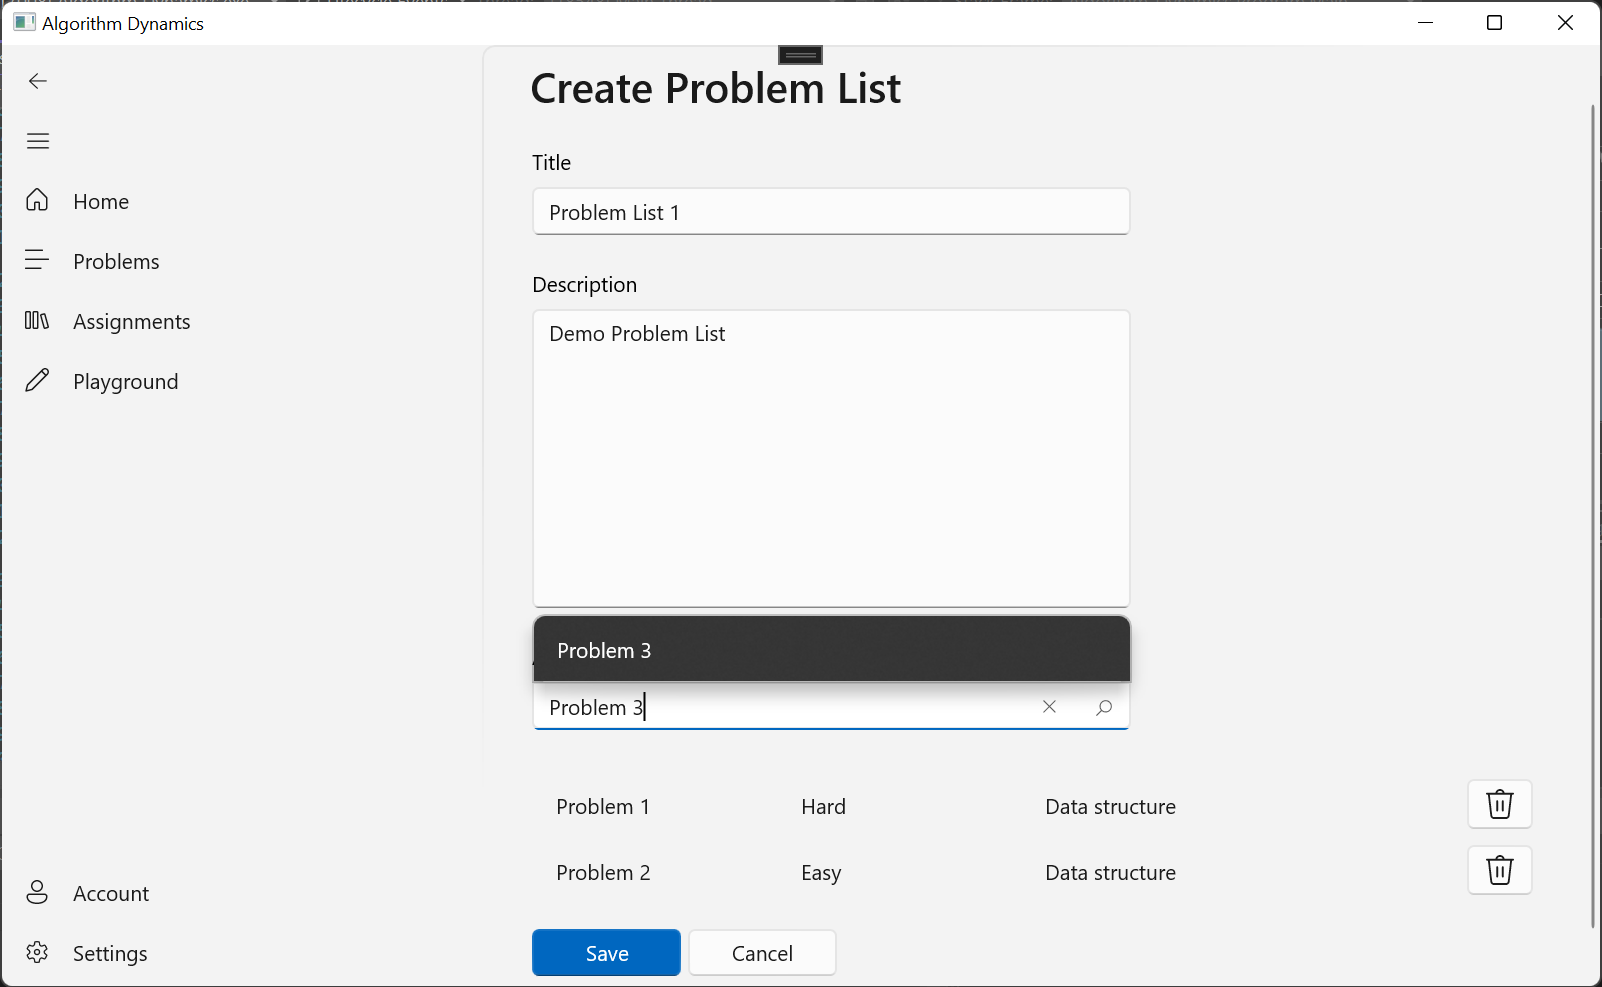
\includegraphics[width=\textwidth, height=\textheight, keepaspectratio]{CreateNewProblemListPage-CreateList}

The title displays correctly, and all fields and the search box is working as intended. I can add and delete problems. When I click the cancel button, I can navigate back to the ProblemsPage correctly. However, when I click the export button, the app crashes.

\begin{minted}{text}
Unhandled exception at 0x00007FFB617D5B2C (CoreMessagingXP.dll) in Algorithm Dynamics.exe: 0xC000027B: An application-internal exception has occurred (parameters: 0x00000281960E3F70, 0x0000000000000001).
\end{minted}

The CoreMessagingXP.dll suggests that this might caused by another internal bug. After doing some research, there is a way around it. I need to obtain the current HWND and set the HWND on the picker\cite{github:WindowsAppSDK:1188}.

\begin{minted}{csharp}
// Get the current window's HWND by passing in the Window object
var hwnd = WinRT.Interop.WindowNative.GetWindowHandle(this);

// Associate the HWND with the file picker
WinRT.Interop.InitializeWithWindow.Initialize(filePicker, hwnd);
\end{minted}

After adding these two lines, the save file picker can work correctly.

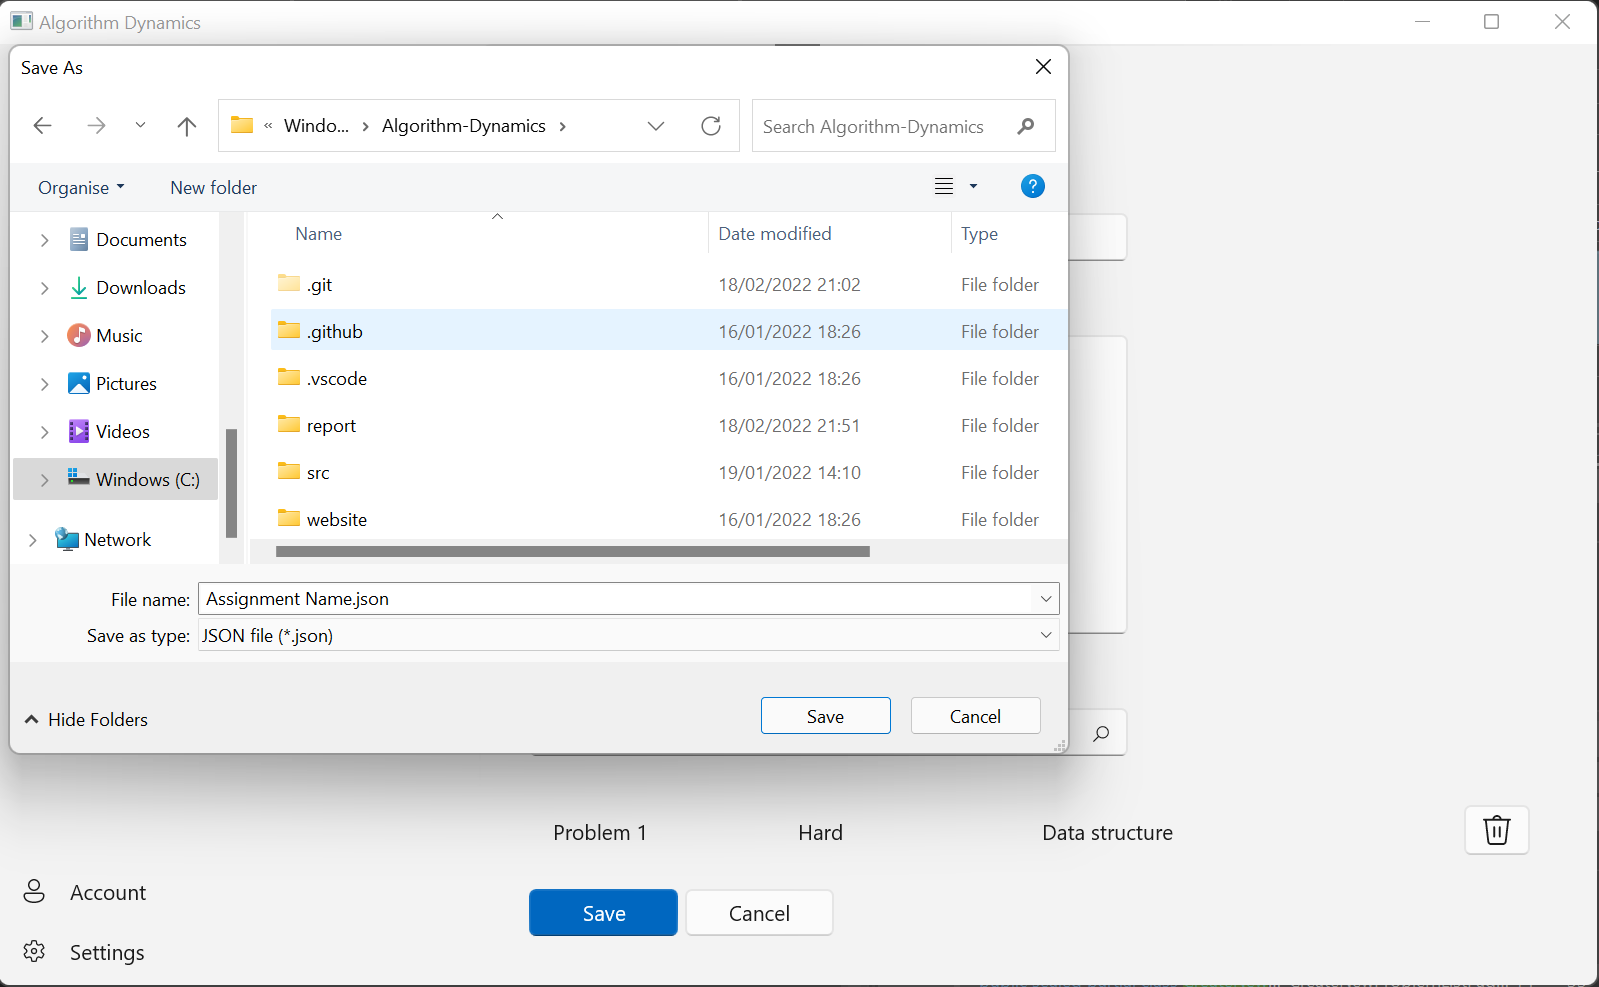
\includegraphics[width=\textwidth, height=\textheight, keepaspectratio]{CreateNewProblemListPage-FilePicker}

\subsubsection{Testing and validation}

\begin{tabulary}{\linewidth}{|L|l|L|}
    \hline
    Test & Result & Remark \\
    \hline
    Does it load & Pass & \\
    \hline
    Does the title field work & Pass &  \\
    \hline
    Does the tags field work & Failed & Marked as a known issue, waiting to be fixed by upstream. \\
    \hline
    Does the difficulty field work & Pass & \\
    \hline
    Does the time limit field work and validate the data & Pass & \\
    \hline
    Does the memory limit field work and validate the data & Pass & \\
    \hline
    Does the description field work & Pass & \\
    \hline
    Does the preview block work & Pass & \\
    \hline
    Is it possible to add or remove test cases & Pass & \\
    \hline
    Does the cancel button work & Pass & \\
    \hline
    Does the save button work & Failed & The save button depends on the database and export function. Which will not be implemented in this iteration. \\
    \hline
\end{tabulary}

\begin{tabulary}{\linewidth}{|L|l|L|}
    \hline
    Does it load & Pass & \\
    \hline
    Does the title field work & Pass & \\
    \hline
    Does the description field work & Pass & \\
    \hline
    Does the search box work & Pass & \\
    \hline
    Does the cancel button work & Pass & \\
    \hline
    Does the save button work & Failed & The save button depends on the database and export function. Which will not be implemented in this iteration. \\
    \hline
    Does the export button work & Pass & The file picker shows up correctly. But similarly, the actual content is not saved to the disk. \\
    \hline
\end{tabulary}

\subsubsection{Stakeholder feedback}

Timofei reports that the spell check is sometimes very annoying and inappropriate in the problem description section.

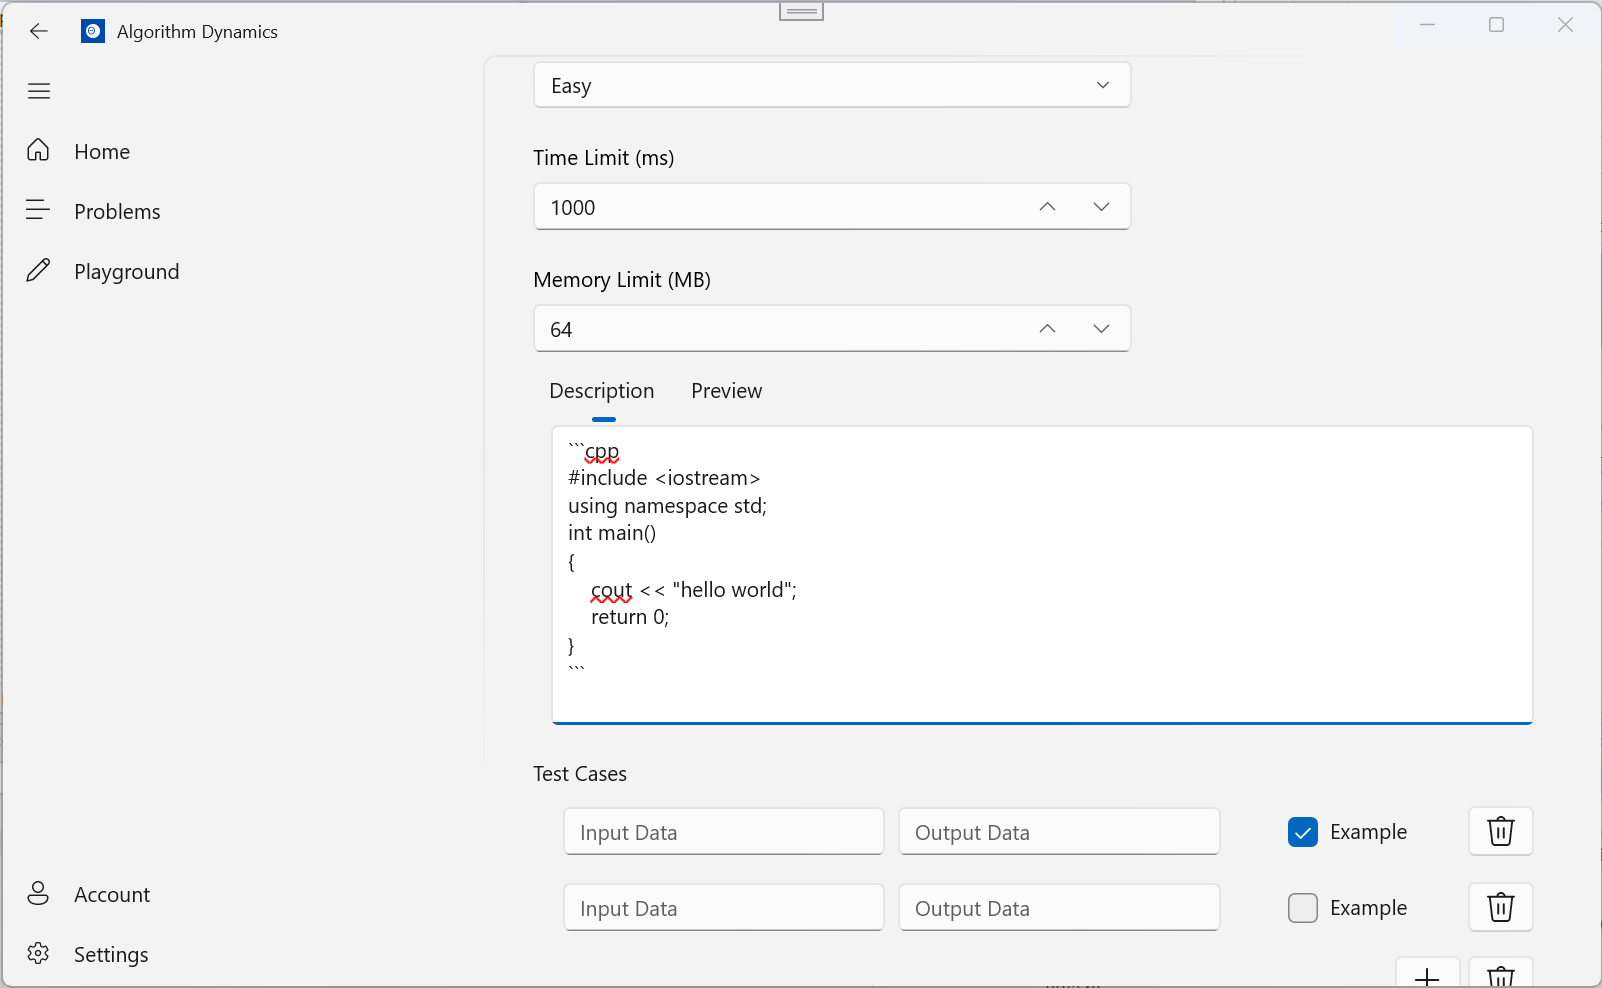
\includegraphics[width=\textwidth, height=\textheight, keepaspectratio]{CreateNewProblemPage-SpellCheck}

Some legal programming language keywords are marked wrong. I decide to disable it since it does not really help much anyway.

\begin{minted}{xml}
<TextBox
    <!-- ... -->
    IsSpellCheckEnabled="False"
    <!-- ... -->/>
\end{minted}

Timofei is happy with the result.

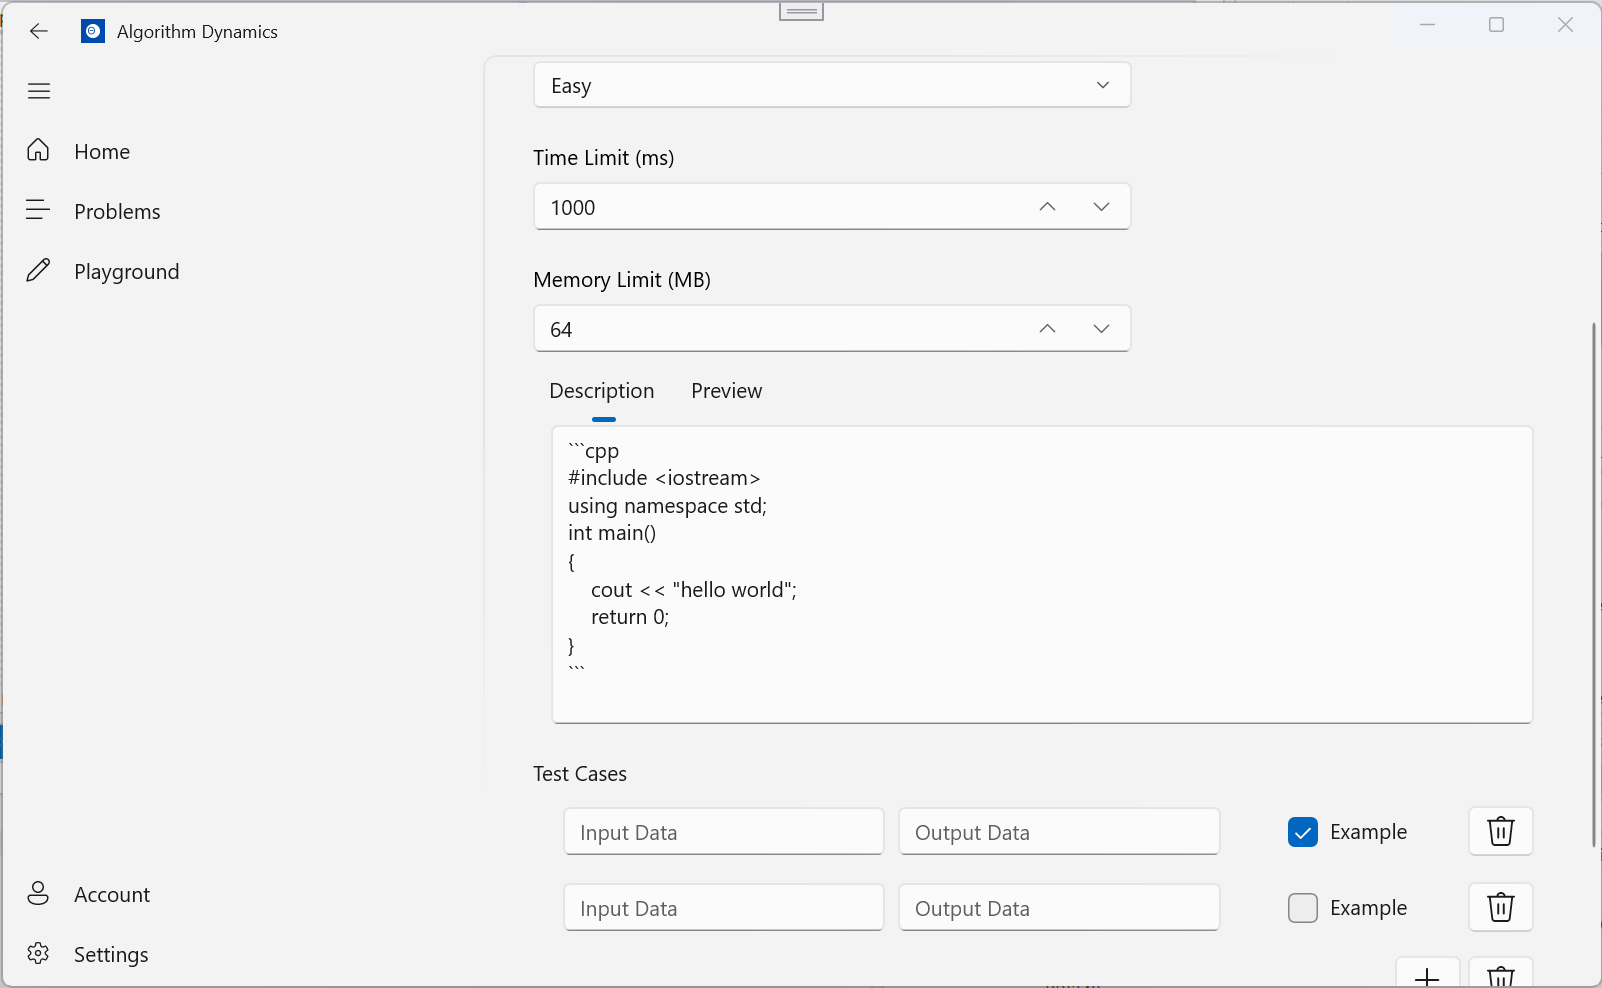
\includegraphics[width=\textwidth, height=\textheight, keepaspectratio]{CreateNewProblemPage-SpellCheck-Disable}

\subsection{Create the AssignmentsPage}

\subsubsection{Implementation}

I first implement the AssignmentsPage, which allows the user to broswe existing assignments. I decide to use a grid of two rows to organize the navigation bar and the assignment list.

\begin{minted}{xml}
<Grid>
    <Grid.RowDefinitions>
        <RowDefinition Height="auto"/>
        <RowDefinition Height="*"/>
    </Grid.RowDefinitions>

    <NavigationView>
        <!-- Navigation Menu -->
    </NavigationView>

    <ListView>
        <!-- Assignment List -->
    </ListView>
</Grid>
\end{minted}

For the navigation panel, it has three tabs, assigned, completed and created. It also has a ComboBox, which allows the user to create or import assignments.

\begin{minted}{xml}
<NavigationView 
    x:Name="AssignmentsNavView"
    IsSettingsVisible="False"
    IsBackButtonVisible="Collapsed"
    IsBackEnabled="False"
    SelectionChanged="AssignmentsNavView_SelectionChanged"
    Header="Header"
    AlwaysShowHeader="False"
    PaneDisplayMode="Top"
    ExpandedModeThresholdWidth="500"
    SelectionFollowsFocus="Disabled"
    IsTabStop="False">
    <NavigationView.MenuItems>
        <NavigationViewItem Content="Assigned" x:Name="AssignedItem"/>
        <NavigationViewItem Content="Completed" x:Name="CompletedItem"/>
        <NavigationViewItem Content="Created" x:Name="CreatedItem"/>
    </NavigationView.MenuItems>

    <NavigationView.PaneFooter>
        <DropDownButton Content="Add">
            <DropDownButton.Flyout>
                <MenuFlyout Placement="Bottom">
                    <MenuFlyoutItem 
                        Text="Create"
                        Click="CreateAssignment"/>
                    <MenuFlyoutItem 
                        Text="Import"
                        Click="ImportAssignment"/>
                </MenuFlyout>
            </DropDownButton.Flyout>
        </DropDownButton>
    </NavigationView.PaneFooter>
</NavigationView>
\end{minted}

I bind the selection changed event to a procedure to switch between different assignment lists.

\begin{minted}{csharp}
/// <summary>
/// Set the <see cref="Assignments"/> based on different SelectedItem
/// </summary>
/// <param name="sender"></param>
/// <param name="args"></param>
private void AssignmentsNavView_SelectionChanged(NavigationView sender, NavigationViewSelectionChangedEventArgs args)
{
    if (AssignmentsNavView.SelectedItem == AssignmentsNavView.MenuItems[0])
    {
        // TODO Query the database and retrieve the assigned assignments
    }
    else if (AssignmentsNavView.SelectedItem == AssignmentsNavView.MenuItems[1])
    {
        // TODO Query the database and retrieve the completed assignments
    }
    else
    {
        // TODO Query the database and retrieve the created assignments
    }
}
\end{minted}

For the CreateAssignment button, when the user clicks it, the App will navigate to the CreateNewProblemListPage with the correct argument so the assignment mode is loaded.

\begin{minted}{csharp}
/// <summary>
/// Navigate to the <see cref="CreateNewProblemListPage"/> with <see cref="CreateNewProblemListPage.Mode.CreateAssignment"/>.
/// </summary>
/// <param name="sender"></param>
/// <param name="e"></param>
private void CreateAssignment(object sender, RoutedEventArgs e)
{
    App.NavigateTo(typeof(CreateNewProblemListPage), Tuple.Create(CreateNewProblemListPage.Mode.CreateAssignment));
}
\end{minted}

For the ImportAssignment button, it shows a similar file picker for the user to pick a file to import.

\begin{minted}{csharp}
/// <summary>
/// Display a <see cref="FileOpenPicker"/> and load the assignment from the file
/// </summary>
/// <param name="sender"></param>
/// <param name="e"></param>
private async void ImportAssignment(object sender, RoutedEventArgs e)
{
    FileOpenPicker filePicker = new FileOpenPicker();

    // Get the current window's HWND by passing in the Window object
    IntPtr hwnd = WindowNative.GetWindowHandle(App.m_window);

    // Associate the HWND with the file picker
    InitializeWithWindow.Initialize(filePicker, hwnd);

    // Use file picker
    filePicker.FileTypeFilter.Add("*");
    StorageFile file = await filePicker.PickSingleFileAsync();
    // TODO Import file into the Database.
}
\end{minted}

For the assignment list, I bind it to an ObserableCollection and display its name and DueDate.

\begin{minted}{xml}
<ListView
    Grid.Row="1"
    SelectionMode="None"
    IsItemClickEnabled="True"
    ItemClick="ListView_ItemClick"
    ItemsSource="{x:Bind Assignments, Mode=OneWay}">
    <ListView.ItemTemplate>
        <DataTemplate x:DataType="local:Assignment">
            <Grid
                Height="50">
                <Grid.ColumnDefinitions>
                    <ColumnDefinition Width="*"/>
                    <ColumnDefinition Width="*"/>
                </Grid.ColumnDefinitions>
                <TextBlock 
                    Grid.Column="0"
                    VerticalAlignment="Center"
                    Text="{x:Bind Name}"/>
                <TextBlock
                    Grid.Column="1"
                    VerticalAlignment="Center"
                    Text="{x:Bind DueDate}"/>
            </Grid>
        </DataTemplate>
    </ListView.ItemTemplate>
</ListView>
\end{minted}

\begin{minted}{csharp}
public ObservableCollection<Assignment> Assignments = new();
\end{minted}

And when an item is clicked, it should navigate to the AssignmentDetailsPage.

\begin{minted}{csharp}
/// <summary>
/// Navigate the the <see cref="AssignmentDetailsPage"/> when an assignment is clicked in the list.
/// </summary>
/// <param name="sender"></param>
/// <param name="e"></param>
private void ListView_ItemClick(object sender, ItemClickEventArgs e)
{
    App.NavigateTo(typeof(AssignmentDetailsPage));
}
\end{minted}

Now, when I run the App, the assignment page is loaded correctly.

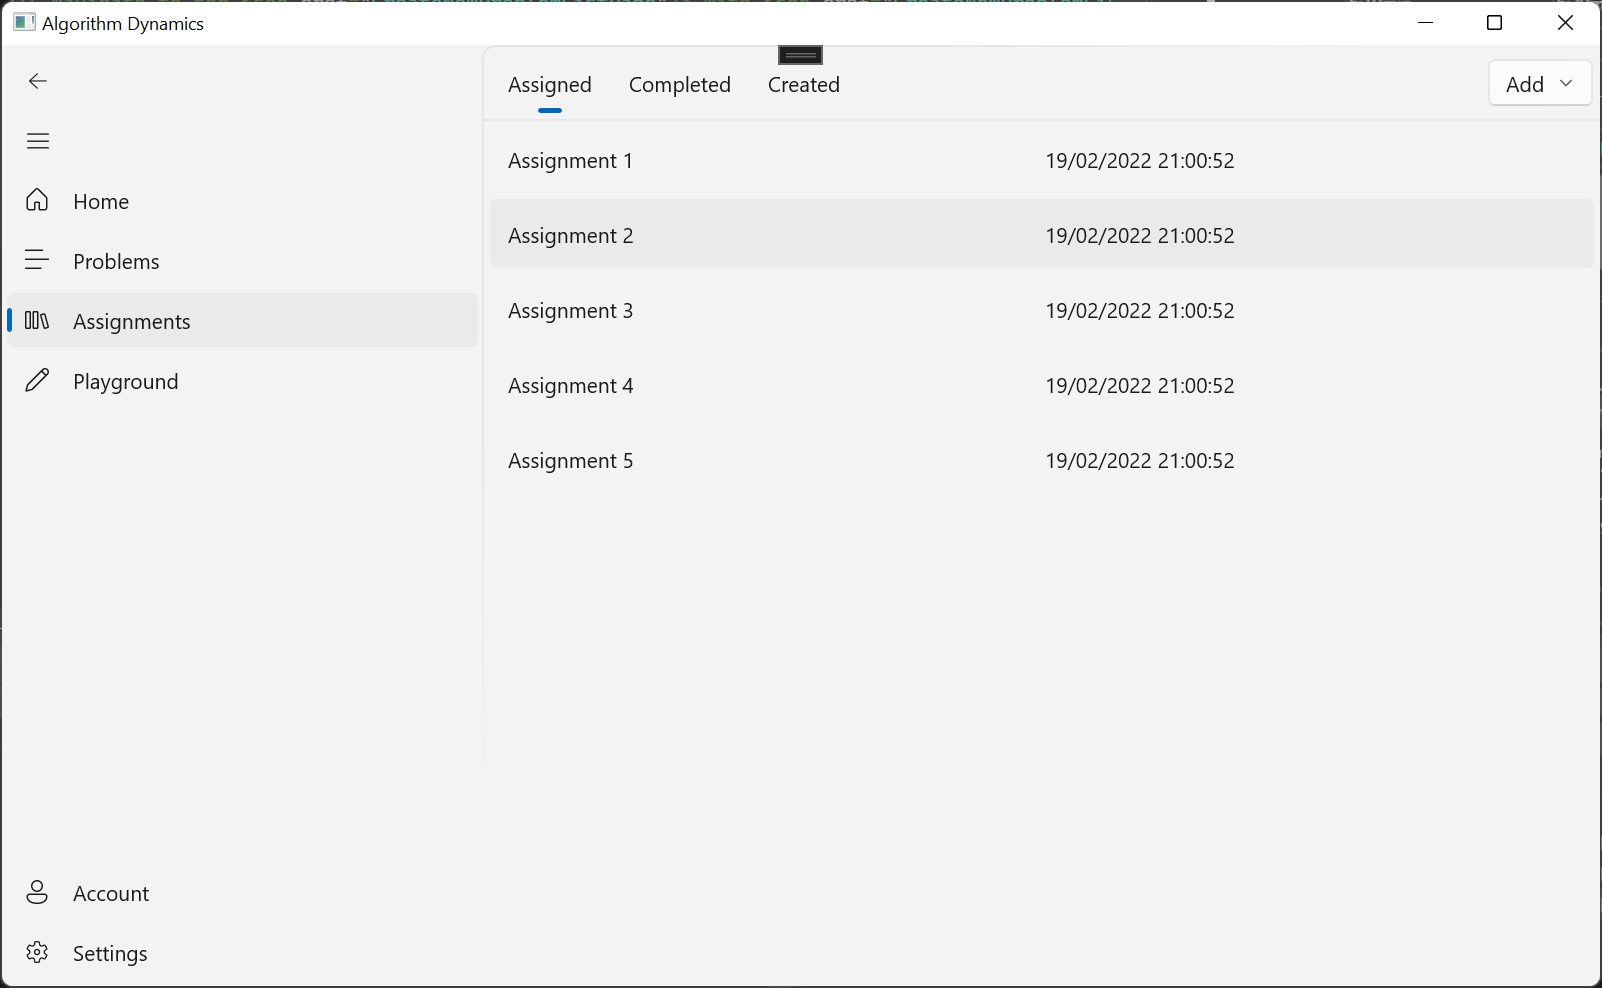
\includegraphics[width=\textwidth, height=\textheight, keepaspectratio]{AssignmentsPage-Layout}

The create button navigates to the CreateProblemListPage with the correct page mode.

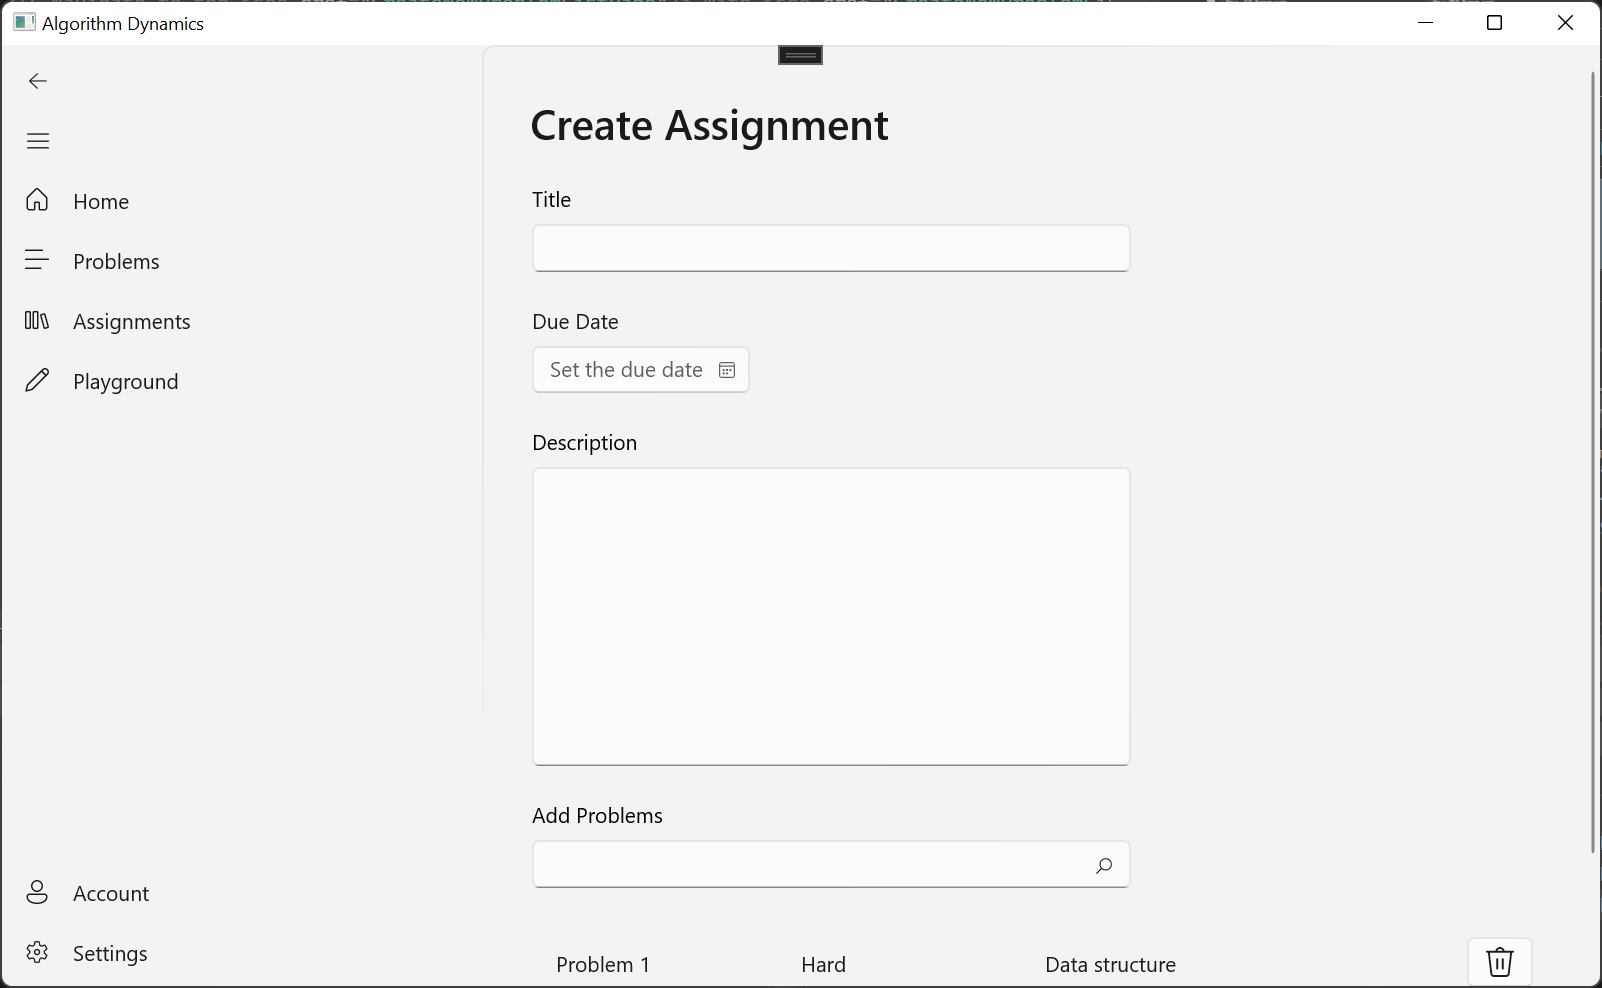
\includegraphics[width=\textwidth, height=\textheight, keepaspectratio]{AssignmentsPage-Create}

The file picker also shows up correctly.

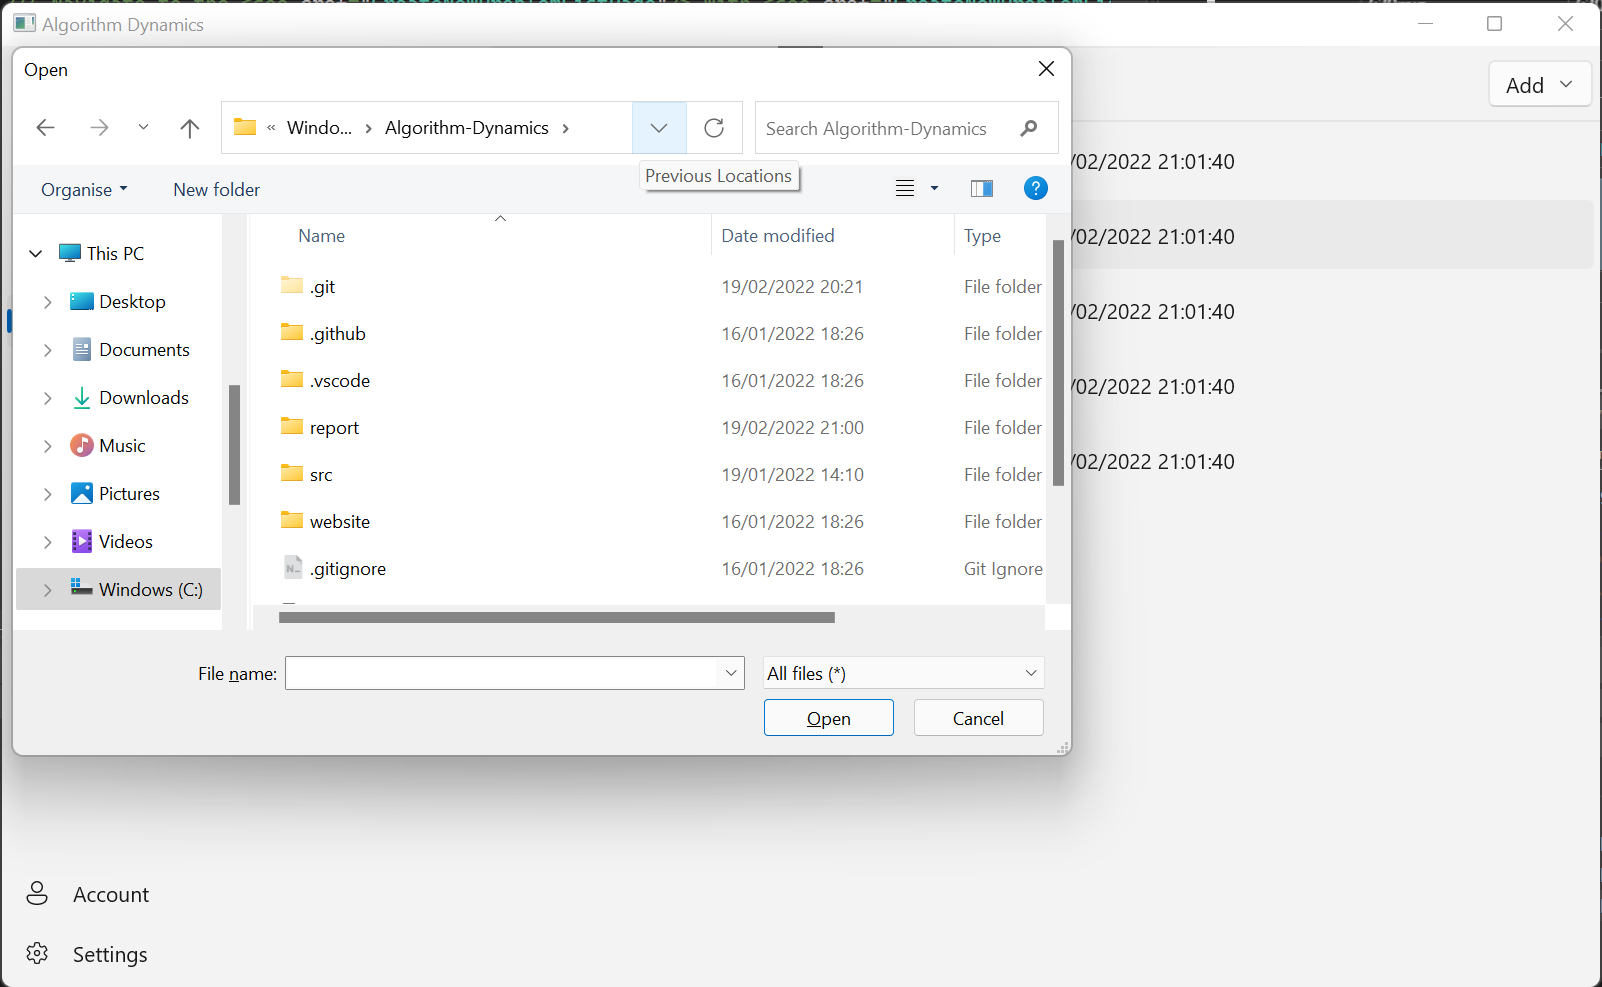
\includegraphics[width=\textwidth, height=\textheight, keepaspectratio]{AssignmentsPage-FilePicker}

Now, I need to create the AssignmentDetailsPage to display the detailed information about each assignment. The AssignmentDetailsPage will be different for the student or the teacher, but I will use the same page mode idea here to reuse as much code as possible.

I wrap everything in a ScrollViewer so all components will be responsive on different screen sizes. In the ScrollViewer, I use a StackPanel to group all components together.

\begin{minted}{xml}
<ScrollViewer>
    <StackPanel
        Margin="32">
        <!-- Main components -->
    </StackPanel>
</ScrollViewer>
\end{minted}

I place a header at the top.

\begin{minted}{xml}
<TextBlock
        Text="Assignment 1"
        Style="{ThemeResource TitleTextBlockStyle}"/>
\end{minted}

Then, a RelativePanel to display all basic information of the assignment.

\begin{minted}{xml}
<RelativePanel>
    <TextBlock 
        Margin="4"
        RelativePanel.AlignLeftWithPanel="True"
        Text="Due 01/01/2022"/>
    <Button
        x:Name="StartButton"
        Margin="4"
        Visibility="{x:Bind _isStudentMode, Mode=OneTime}"
        RelativePanel.LeftOf="SubmitButton"
        Content="Start"/>
    <Button
        x:Name="SubmitButton"
        Content="Submit"
        Margin="4"
        Visibility="{x:Bind _isStudentMode, Mode=OneTime}"
        RelativePanel.AlignRightWithPanel="True"
        Style="{ThemeResource AccentButtonStyle}"/>
    <Button
        x:Name="EditButton"
        Content="Edit"
        Margin="4"
        Click="EditAssignment"
        Visibility="{x:Bind _isTeacherMode, Mode=OneTime}"
        RelativePanel.LeftOf="ImportSubmissionButton"/>
    <Button
        x:Name="ImportSubmissionButton"
        Content="Import Submission"
        Margin="4"
        Visibility="{x:Bind _isTeacherMode, Mode=OneTime}"
        RelativePanel.AlignRightWithPanel="True"
        Style="{ThemeResource AccentButtonStyle}"/>
</RelativePanel>
\end{minted}

A two by two grid to put the description of the assignment, the problem list and the submission list.

\begin{minted}{xml}
<Grid>
    <Grid.RowDefinitions>
        <RowDefinition Height="auto"/>
        <RowDefinition Height="*"/>
    </Grid.RowDefinitions>
    <Grid.ColumnDefinitions>
        <ColumnDefinition Width="*"/>
        <ColumnDefinition Width="*"/>
    </Grid.ColumnDefinitions>
    <TextBlock 
        Grid.Row="0"
        Grid.Column="0"
        TextWrapping="Wrap"
        Margin="4"
        Text="Description."/>
    <ListView
        x:Name="ProblemListView"
        Grid.Row="1"
        Grid.Column="0"
        Header="Problems"
        IsItemClickEnabled="True"
        ItemClick="ProblemListView_ItemClick"
        ItemsSource="{x:Bind Problems, Mode=OneWay}"
        Margin="4">
        <ListView.ItemTemplate>
            <DataTemplate x:DataType="local:Problem">
                <TextBlock Text="{x:Bind Name, Mode=OneWay}"/>
            </DataTemplate>
        </ListView.ItemTemplate>
    </ListView>
    <ListView
        Grid.Row="0"
        Grid.RowSpan="2"
        Grid.Column="1"
        Margin="4"
        Visibility="{x:Bind _isTeacherMode, Mode=OneTime}"
        ItemsSource="{x:Bind Submissions, Mode=OneWay}"
        Header="Submissions">
        <ListView.ItemTemplate>
            <DataTemplate x:DataType="local:Submission">
                <TextBlock Text="{x:Bind Status, Mode=OneWay}"/>
            </DataTemplate>
        </ListView.ItemTemplate>
    </ListView>
</Grid>
\end{minted}

Similarly, I use the PageMode to manage visibility for different components, therefore display a different page for students and teachers.

\begin{minted}{csharp}
public enum Mode
{
    Student,
    Teacher
}
private Mode _pageMode = Mode.Student;
private bool _isStudentMode { get => _pageMode == Mode.Student; }
private bool _isTeacherMode { get => _pageMode == Mode.Teacher; }

/// <summary>
/// Handle the Navigation Arguments
/// Set the <see cref="_pageMode"/> if the Parameter is not <see cref="null"/>.
/// </summary>
/// <param name="e"></param>
protected override void OnNavigatedTo(NavigationEventArgs e)
{
    if (e.Parameter != null)
    {
        _pageMode = ((Tuple<Mode>)e.Parameter).Item1;
    }
    base.OnNavigatedTo(e);
}
\end{minted}

I can modify the navigate function in the AssignmentsPage to pass the correct argument for corresponding assignment.

\begin{minted}{csharp}
/// <summary>
/// Navigate the the <see cref="AssignmentDetailsPage"/> when an assignment is clicked in the list.
/// </summary>
/// <param name="sender"></param>
/// <param name="e"></param>
private void ListView_ItemClick(object sender, ItemClickEventArgs e)
{
    // TODO use logged in user information to determine which page to display 
    var assignment = e.ClickedItem as Assignment;
    if (assignment.Description == "Created Assignment")
    {
        App.NavigateTo(typeof(AssignmentDetailsPage), Tuple.Create(AssignmentDetailsPage.Mode.Teacher));
    }
    else
    {
        App.NavigateTo(typeof(AssignmentDetailsPage), Tuple.Create(AssignmentDetailsPage.Mode.Student));
    }
}
\end{minted}

When I click the assignments under the Assigned panel, the student view with the correct submit button shows up correctly.

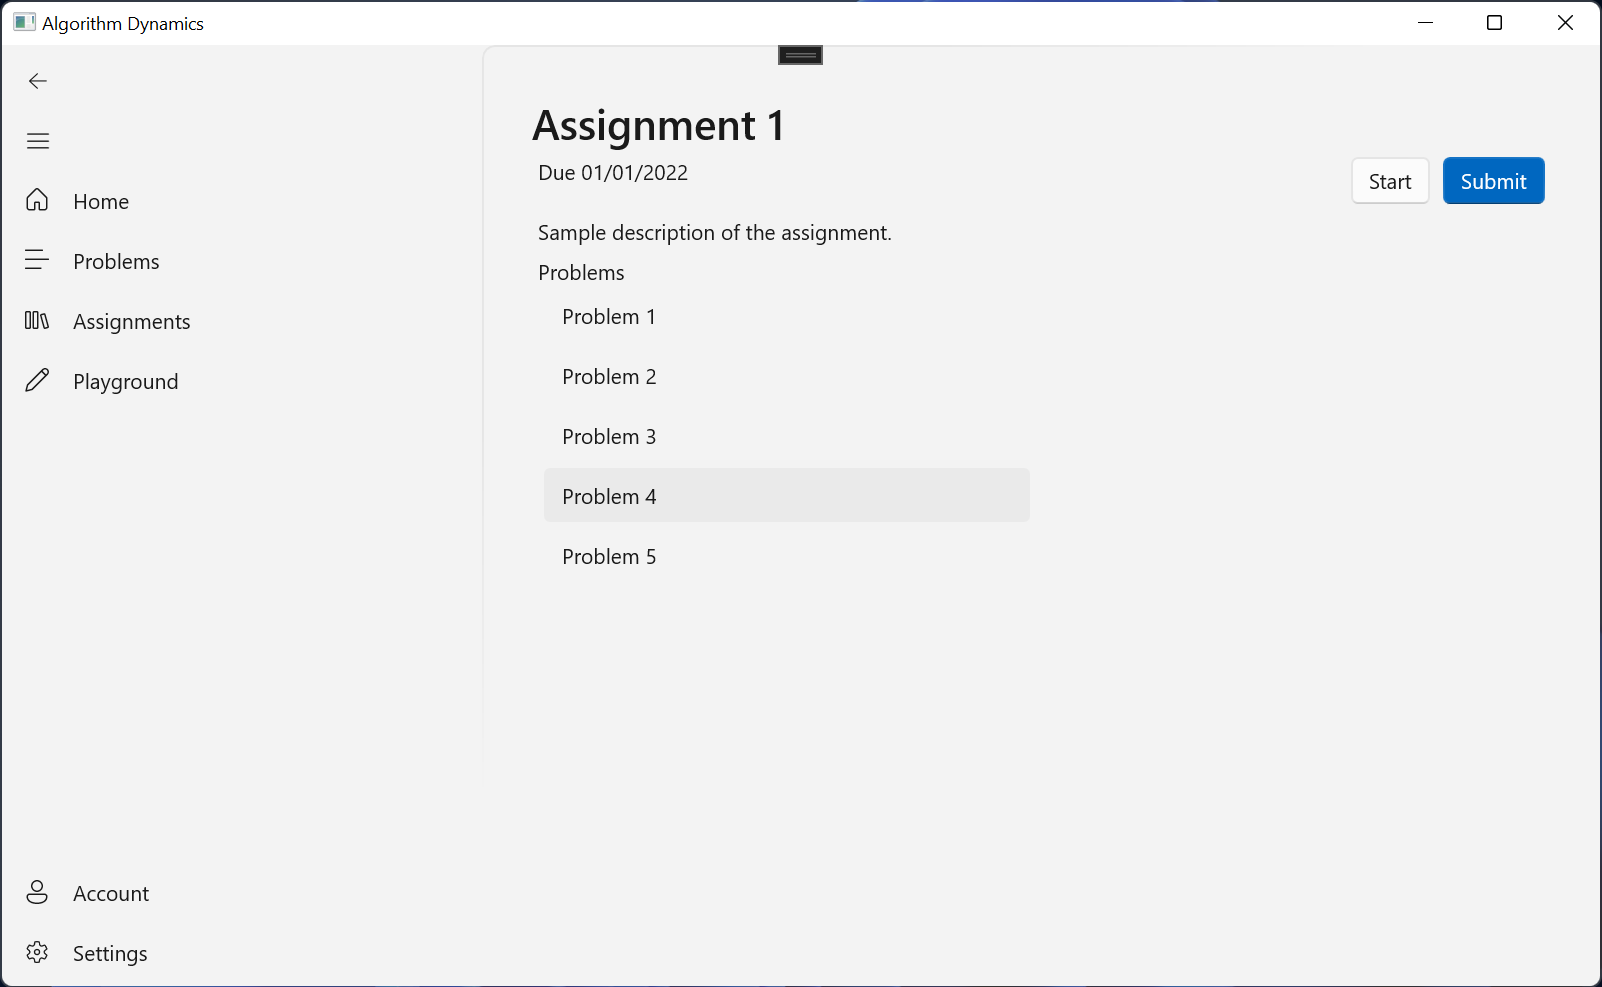
\includegraphics[width=\textwidth, height=\textheight, keepaspectratio]{AssignmentDetailsPage-Student}

When I click the assignments under the Created panel, the teacher view with the correct buttons and submissions shows up correctly.

\includegraphics[width=\textwidth, height=\textheight, keepaspectratio]{AssignmentDetailsPage-Teacher}

All these buttons are not working right now, since the UI is the only thing that will be implemented in this iteration.

\subsubsection{Testing and validation}

\begin{tabulary}{\linewidth}{|L|l|L|}
    \hline
    Test & Result & Remark \\
    \hline
    Does it load & Pass & \\
    \hline
    Does the navigation panel work & Pass &  \\
    \hline
    Does the import button work & Failed & The import function will not be implemented in this iteration.  \\
    \hline
    Does the create button work & Pass & \\
    \hline
    Does the assignment details navigation work & Pass & \\
    \hline
    Does different page modes work & Pass & \\
    \hline
    Does the description show up correctly & Pass & \\
    \hline
    Does the problem list show up correctly & Pass & \\
    \hline
    Does the submission list show up correctly & Pass & \\
    \hline
    Does the due date show up correctly & Pass & \\
    \hline
    Does the start button work & Pass & \\
    \hline
    Does the submit button work & Failed & The export function will not be implemented in this iteration. \\
    \hline
    Does the edit button work & Pass & \\
    \hline
    Does the judge button work & Failed & The Judger will not be implemented in this iteration. \\
    \hline
    Does the export button work & Failed & The export function will not be implemented in this iteration. \\
    \hline
\end{tabulary}

\subsubsection{Stakeholder feedback}

When I show the assignment pages to Mr Grimwood, he asked me that how the student's submission is graded? Is it send to a server or is it graded locally. I explained that the code submission will be compiled and run locally against test cases. He then expressed concerns of the security of the grading system. Allowing any external code to be run on the teacher's computer may not be a good idea.

He showed this example to me:

\begin{minted}{python}
import os
os.system("calc")
\end{minted}

When executing this Python code, the system calculator will be launched. The \code{calc} command can be replaced with any other commands, such as deleting files or shutting down the computer.

After some research, there is no easy way on Windows to restrictive the priviliges for certain code. Since this security issue is very serious, we both agree that implementing the assignment feature in this way is not ideal.

For now, I will discontinue all the assignment related feature in the prototype. I will continue researching and discuss some potintial solutions in the Evaluation chapter.

\subsection{Create the SettingsPage}

\subsubsection{Implementation}

Similarly, I wrap a ScrollViewer around all the components so they can be responsive to different screen size.

\begin{minted}{xml}
<ScrollViewer>
    <StackPanel
        Margin="32">
        <!-- ... -->
    </StackPanel>
</ScrollViewer>
\end{minted}

For the theme selection, I use three radio buttons so the user can select between different themes easily.

\begin{minted}{xml}
<TextBlock
    Style="{ThemeResource SubtitleTextBlockStyle}"
    Margin="0 12 0 0"
    FontWeight="Normal"
    Text="Theme Mode" />
<StackPanel x:Name="ThemePanel" Margin="0 10 0 0">
    <RadioButton 
        Tag="Light" 
        Content="Light"
        Checked="ThemeRadioButton_Checked"/>
    <RadioButton 
        Tag="Dark" 
        Content="Dark"
        Checked="ThemeRadioButton_Checked"/>
    <RadioButton 
        Tag="Default" 
        Content="Use system settings"
        Checked="ThemeRadioButton_Checked"/>
</StackPanel>
\end{minted}

The radio buttons are bind to a procedure, so when they are checked, the subroutine gets executed.

\begin{minted}{csharp}
/// <summary>
/// Change the application request theme to the selected theme when the radio button is clicked
/// </summary>
/// <param name="sender"></param>
/// <param name="e"></param>
private void ThemeRadioButton_Checked(object sender, RoutedEventArgs e)
{
    var selectedTheme = ((RadioButton)sender)?.Tag?.ToString();

    if (selectedTheme != null && App.m_window.Content is FrameworkElement rootElement)
    {
        rootElement.RequestedTheme = GetEnum<ElementTheme>(selectedTheme);
    }
}
\end{minted}

The run code time limit and memory limit are two simple number box, which automatically validate the input.

\begin{minted}{xml}
<TextBlock
    Style="{ThemeResource SubtitleTextBlockStyle}"
    Margin="0 20 0 0"
    FontWeight="Normal"
    Text="Run Code Time Limit" />
<StackPanel 
    Margin="0 10 0 0"
    Orientation="Horizontal">
    <NumberBox
        SpinButtonPlacementMode="Inline"
        Value="1000"
        Minimum="100"
        SmallChange="100"
        LargeChange="500" />
    <TextBlock 
        Margin="8"
        Text="ms"
        VerticalAlignment="Center"/>
</StackPanel>
<TextBlock
    Style="{ThemeResource SubtitleTextBlockStyle}"
    Margin="0 20 0 0"
    FontWeight="Normal"
    Text="Run Code Memory Limit" />
<StackPanel 
    Margin="0 10 0 0"
    Orientation="Horizontal">
    <NumberBox
        Value="64"
        Minimum="16"
        SpinButtonPlacementMode="Inline"
        SmallChange="64"
        LargeChange="256" />
    <TextBlock
        Margin="8"
        Text="MB"
        VerticalAlignment="Center"/>
</StackPanel>
\end{minted}

I use an expander to hold the programming language configuration editor. It expands when the user clicks it, which makes the interface looks simple when the user does not want to modify this part of settings.

\begin{minted}{xml}
<TextBlock
    Style="{ThemeResource SubtitleTextBlockStyle}"
    Margin="0 20 0 0"
    FontWeight="Normal"
    Text="Preferred Programming Language" />
<Expander
    Margin="0 20 0 0"
    IsExpanded="False">
    <Expander.Header>
        <StackPanel 
            Orientation="Horizontal">
            <ComboBox
                VerticalAlignment="Stretch"
                Margin="2"
                SelectedIndex="0">
                <x:String>C</x:String>
                <x:String>C++</x:String>
                <x:String>Python</x:String>
            </ComboBox>
            <Button 
                x:Name="AddLangButton"
                ToolTipService.ToolTip="Add a new Programming Language configuration"
                Margin="2"
                Click="AddLangButton_Click">
                <Button.Content>
                    <SymbolIcon Symbol="Add"/>
                </Button.Content>
            </Button>
            <Button 
                ToolTipService.ToolTip="Delete the selected configuration"
                Margin="2">
                <Button.Content>
                    <SymbolIcon Symbol="Delete"/>
                </Button.Content>
                <Button.Flyout>
                    <Flyout>
                        <StackPanel>
                            <TextBlock 
                                Style="{ThemeResource BaseTextBlockStyle}"
                                Text="The selected language configuration will be deleted. Do you want to continue?" Margin="0 0 0 12" />
                            <Button 
                                HorizontalAlignment="Right"
                                Content="Yes" />
                        </StackPanel>
                    </Flyout>
                </Button.Flyout>
            </Button>
        </StackPanel>
    </Expander.Header>
    <Expander.Content>
        <StackPanel
            HorizontalAlignment="Stretch"
            MinWidth="400">
            <TextBox
                x:Name="DisplayNameTextBox"
                Header="Display Name"/>
            <TextBox
                x:Name="LanguageCodeTextBox"
                Header="Language Code"
                Margin="0 4 0 0"/>
            <CheckBox
                x:Name="NeedCompileCheckBox"
                Content="Need Compile"
                Margin="0 4 0 0"/>
            <TextBox
                x:Name="CompileCommandTextBox"
                Visibility="{x:Bind NeedCompileCheckBox.IsChecked, Mode=OneWay}"
                Header="Compile Command"
                Margin="0 4 0 0"/>
            <TextBox
                x:Name="CompileArgumentTextBox"
                Visibility="{x:Bind NeedCompileCheckBox.IsChecked, Mode=OneWay}"
                Header="Compile Argument"
                Margin="0 4 0 0"/>
            <TextBox
                x:Name="RunCommandTextBox"
                Header="Run Command"
                Margin="0 4 0 0"/>
            <TextBox
                x:Name="RunArgumentsTextBox"
                Header="Run Arguments"
                Margin="0 4 0 0"/>
            <TextBox
                x:Name="FileExtensionTextBox"
                PlaceholderText=".*"
                Header="File Extension"
                Margin="0 4 0 0"/>
            <StackPanel 
                Margin="0 16 0 0"
                Orientation="Horizontal">
                <Button
                    Content="Save"
                    Style="{ThemeResource AccentButtonStyle}">
                </Button>
            </StackPanel>
        </StackPanel>
    </Expander.Content>
</Expander>
\end{minted}

At the bottom, I put up some links about the project and a disclaimer.

\begin{minted}{xml}
<TextBlock
    Style="{ThemeResource SubtitleTextBlockStyle}"
    Margin="0 20 0 0"
    FontWeight="Normal"
    Text="About" />
<HyperlinkButton 
    Margin="0 4 0 0"
    Content="GitHub"
    NavigateUri="https://github.com/HEIGE-PCloud/Algorithm-Dynamics"/>
<HyperlinkButton 
    Margin="0 4 0 0"
    Content="Website"
    NavigateUri="https://algorithmdynamics.com/"/>
<HyperlinkButton 
    Margin="0 4 0 0"
    Content="Report"
    NavigateUri="https://algorithmdynamics.com/report.pdf"/>
<TextBlock
    Style="{ThemeResource SubtitleTextBlockStyle}"
    Margin="0 20 0 0"
    FontWeight="Normal"
    Text="Disclaimer" />
<RichTextBlock>
    <Paragraph>THIS CODE AND INFORMATION IS PROVIDED 'AS IS' WITHOUT WARRANTY OF ANY KIND, EITHER EXPRESSED OR IMPLIED, INCLUDING BUT NOT LIMITED TO THE IMPLIED WARRANTIES OF MERCHANTABILITY AND/OR FITNESS FOR A PARTICULAR PURPOSE.</Paragraph>
</RichTextBlock>
\end{minted}

All the data should be immediately saved to the disk after the user changes a value. For now, the data will not be saved to the disk as the settings module will not be implemented in this iteration.

\includegraphics[width=\textwidth, height=\textheight, keepaspectratio]{SettingsPage-Light}

\includegraphics[width=\textwidth, height=\textheight, keepaspectratio]{SettingsPage-Dark}

\subsubsection{Testing and validation}

\begin{tabulary}{\linewidth}{|L|l|L|}
    \hline
    Does it load & Pass & \\
    \hline
    Does theme switch work & Pass & \\
    \hline
    Does the run code time limit field work and validate the data & Pass & \\
    \hline
    Does the run code memory limit field work and validate the data & Pass & \\
    \hline
    Does the language configuration editor works & Pass & \\
    \hline
    Does the about buttons work & Pass & \\
    \hline
    Does the settings get loaded and saved correctly & Failed & The core of the settings module will be implemented in a later iteration. \\
    \hline
\end{tabulary}

\subsubsection{Stakeholder feedback}

PCloud says that it will be great if a ``Clear history data'' button is placed in the settings page, so he can reset his statistics or problems easily. This will be a useful feature and very easy to implement.

\begin{minted}{xml}
<StackPanel 
    Margin="0 10 0 0"
    Orientation="Vertical">
    <Button
    x:Name="ClearAllSubmissionsButton"
    Margin="0 4 0 0"
    Content="Clear Submission History">
    <Button.Flyout>
        <Flyout x:Name="ClearAllSubmissionsFlyout">
        <StackPanel>
            <TextBlock 
            Style="{ThemeResource BaseTextBlockStyle}" 
            Text="All submission history will be deleted. Do you want to continue?" 
            Margin="0,0,0,12"/>
            <Button 
            HorizontalAlignment="Right" 
            Content="Yes"
            Click="DeleteAllSubmissions"/>
        </StackPanel>
        </Flyout>
    </Button.Flyout>
    </Button>
    <Button
    x:Name="ClearAllProblemsButton"
    Margin="0 4 0 0"
    Content="Clear All Problems">
    <Button.Flyout>
        <Flyout x:Name="ClearAllProblemsFlyout">
        <StackPanel>
            <TextBlock 
            Style="{ThemeResource BaseTextBlockStyle}" 
            Text="All problems will be deleted. Do you want to continue?" 
            Margin="0,0,0,12"/>
            <Button 
            HorizontalAlignment="Right" 
            Content="Yes"
            Click="DeleteAllProblems"/>
        </StackPanel>
        </Flyout>
    </Button.Flyout>
    </Button>
    <Button
    x:Name="ClearAllDataButton"
    Margin="0 4 0 0"
    Content="Clear All Data">
    <Button.Flyout>
        <Flyout x:Name="ClearAllDataFlyout">
        <StackPanel>
            <TextBlock 
            Style="{ThemeResource BaseTextBlockStyle}" 
            Text="All data will be deleted. Do you want to continue?" 
            Margin="0,0,0,12"/>
            <TextBlock 
            Text="Restart is required."/>
            <Button 
            HorizontalAlignment="Right" 
            Content="Yes"
            Click="ClearAllData"/>
        </StackPanel>
        </Flyout>
    </Button.Flyout>
    </Button>
</StackPanel>
\end{minted}

I add three buttons to the settings page, one to clear all submissions, one to clear all problems, and one to clear all data. They will be connected to the database functions in the later milestone.

\includegraphics[width=\textwidth, height=\textheight, keepaspectratio]{SettingsPage-ClearData}

\subsection{Stakeholder feedback}

My stakeholders are generally very happy about the user interface of the software. They think the prototype looks modern and easy to use. They cannot wait to see the full functionality of the software.

\end{document}